%%%%%%%% ICML 2019 EXAMPLE LATEX SUBMISSION FILE %%%%%%%%%%%%%%%%%

\documentclass{article}

% Recommended, but optional, packages for figures and better typesetting:
\usepackage{microtype}
\usepackage{graphicx}
\usepackage{subfigure}
\usepackage{booktabs} % for professional tables

% hyperref makes hyperlinks in the resulting PDF.
% If your build breaks (sometimes temporarily if a hyperlink spans a page)
% please comment out the following usepackage line and replace
% \usepackage{icml2019} with \usepackage[nohyperref]{icml2019} above.
\usepackage{hyperref}

% Attempt to make hyperref and algorithmic work together better:
\newcommand{\theHalgorithm}{\arabic{algorithm}}

% Use the following line for the initial blind version submitted for review:
\usepackage{icml2019}

% If accepted, instead use the following line for the camera-ready submission:
%\usepackage[accepted]{icml2019}

% The \icmltitle you define below is probably too long as a header.
% Therefore, a short form for the running title is supplied here:
\icmltitlerunning{On the Generalization Performance of Compressed Word Embeddings}

%Added by Avner
\usepackage{amsmath,amsfonts,amsthm,amssymb}

%\usepackage{graphicx}
%\usepackage{amsmath,amsfonts,amssymb,amsopn,amsbsy,amsthm}
%\usepackage{dsfont,bm,bbm,times,url,verbatim,epstopdf,xspace}
%\usepackage[capitalize]{cleveref}
%\usepackage{placeins}
%\usepackage{amssymb,amsthm}
%\usepackage{bbm,epstopdf}
%\usepackage[group-separator={,}]{siunitx}
%\usepackage[export]{adjustbox}
%\usepackage{hhline}
%\usepackage[hypertexnames=false]{hyperref}
% for footnotes without markers
%\newcommand\blfootnote[1]{%
%  \begingroup
%  \renewcommand\thefootnote{}\footnote{#1}%
%  \addtocounter{footnote}{-1}%
%  \endgroup
%}

%\newcommand{\vfigsp}{\vspace{-0.5em}}
%\newcommand{\vflistsp}{\vspace{-0.25em}}
\newcommand{\vfigsp}{}
\newcommand{\vflistsp}{}

% New commands added from Nystrom notes.
\newcommand{\Nystrom}{Nystr\"{o}m }
\newcommand{\NystromNS}{Nystr\"{o}m} % NS means ``no space''
\newcommand{\NystromCaps}{NYSTR\"{O}M }
\newcommand{\NystromCapsNS}{NYSTR\"{O}M} % NS means ``no space''
\newcommand{\Ap}{A^\perp}
\newcommand{\mua}{\mu_A}
\newcommand{\muap}{\mu_{\Ap}}
\newcommand{\bphi}{\bar{\phi}}
\newcommand{\by}{\bar{y}}
\newcommand{\bS}{\bar{S}}
\newcommand{\bT}{\bar{T}}
%\newcommand{\bw}{\bar{w}}
%\newcommand{\bv}{\bar{v}}
%\newcommand{\bF}{\bar{F}}
%\newcommand{\bg}{\bar{g}}
%\newcommand{\be}{\bar{\eta}}
%\newcommand{\br}{\bar{\rho}}
%\newcommand{\bU}{\bar{U}}
%\newcommand{\bV}{\bar{V}}
%\newcommand{\bLam}{\bar{\Lambda}}
%\newcommand{\bL}{\bar{L}}
\newcommand{\hx}{\hat{x}}
\newcommand{\hb}{\hat{b}}
%\newcommand{\hX}{\hat{X}}
%\newcommand{\hY}{\hat{Y}}
\newcommand{\hp}{\hat{\phi}}
\newcommand{\hK}{\hat{K}}
%\newcommand{\tp}{\tilde{\phi}}
\newcommand{\tk}{\tilde{k}}
%\newcommand{\tC}{\tilde{C}}
\newcommand{\eps}{\epsilon}
\newcommand{\teps}{\tilde{\epsilon}}
\newcommand{\tS}{\tilde{S}}
\newcommand{\tK}{\tilde{K}}
\newcommand{\tZ}{\tilde{Z}}
\newcommand{\tA}{\tilde{A}}
\newcommand{\tf}{\tilde{f}}
\newcommand{\tz}{\tilde{z}}
\newcommand{\tsigma}{\tilde{\sigma}}
\newcommand{\tgamma}{\tilde{\gamma}}
\newcommand{\tlambda}{\tilde{\lambda}}
\newcommand{\hcR}{\widehat{\cR}}
\newcommand{\id}{I}
\newcommand{\sq}{\sqrt{2}}
\newcommand{\ulq}{\underline{q}}
\newcommand{\olq}{\overline{q}}
\newcommand*{\QED}{\hfill\ensuremath{\square}}
\DeclareMathOperator*{\argmin}{arg\,min}
\DeclareMathOperator*{\argmax}{arg\,max}
\DeclareMathOperator*{\rank}{rank}

\newcommand*\conj[1]{\overline{#1}}

% note: I removed the package amsthm because it defines "proof", which is already defined in jmlr2e package
\newcommand{\ie}{i.e.}
\newcommand{\eg}{e.g.}
\newcommand{\etal}{et al.\ }
\newcommand{\etalNS}{et al.}

\def\ddefloop#1{\ifx\ddefloop#1\else\ddef{#1}\expandafter\ddefloop\fi}
%
%% \bbA, \bbB, ...
\def\ddef#1{\expandafter\def\csname bb#1\endcsname{\ensuremath{\mathbb{#1}}}}
\ddefloop ABCDEFGHIJKLMNOPQRSTUVWXYZ\ddefloop
%
%% \bfA, \bfB, ...
%\def\ddef#1{\expandafter\def\csname bf#1\endcsname{\ensuremath{\mathbf{#1}}}}
%\ddefloop ABCDEFGHIJKLMNOPQRSTUVWXYZabcdefghijklmnopqrstuvwxyz\ddefloop
%
%% \bfalpha, \bfbeta, ...,  \bfGamma, \bfDelta, ...,
%\def\ddef#1{\expandafter\def\csname bf#1\endcsname{\ensuremath{\pmb{\csname #1\endcsname}}}}
%\ddefloop {alpha}{beta}{gamma}{delta}{epsilon}{varepsilon}{zeta}{eta}{theta}{vartheta}{iota}{kappa}{lambda}{mu}{nu}{xi}{pi}{varpi}{rho}{varrho}{sigma}{varsigma}{tau}{upsilon}{phi}{varphi}{chi}{psi}{omega}{Gamma}{Delta}{Theta}{Lambda}{Xi}{Pi}{Sigma}{varSigma}{Upsilon}{Phi}{Psi}{Omega}{ell}\ddefloop
%
%% \cA, \cB, ...
\def\ddef#1{\expandafter\def\csname c#1\endcsname{\ensuremath{\mathcal{#1}}}}
\ddefloop ABCDEFGHIJKLMNOPQRSTUVWXYZ\ddefloop
%
%% \mbf0, \mbf1, ...
%\newcommand\mbf{\ensuremath{\mathbf}}
%
%\DeclareMathOperator*{\argmin}{arg\,min}
%\DeclareMathOperator*{\argmax}{arg\,max}
%
%\newcommand\parens[1]{(#1)}
\newcommand\norm[1]{\|#1\|}
%\newcommand\braces[1]{\{#1\}}
%\newcommand\brackets[1]{[#1]}
%\newcommand\ceil[1]{\lceil#1\rceil}
%\newcommand\abs[1]{|#1|}
%\newcommand\ind[1]{\ensuremath{\mathds{1}\{#1\}}}
\newcommand\dotp[1]{\langle #1 \rangle}
%\newcommand\Parens[1]{\left(#1\right)}
%\newcommand\Norm[1]{\left\|#1\right\|}
%\newcommand\Braces[1]{\left\{#1\right\}}
%\newcommand\Brackets[1]{\left[#1\right]}
%\newcommand\Ceil[1]{\left\lceil#1\right\rceil}
%\newcommand\Abs[1]{\left|#1\right|}
%\newcommand\Ind[1]{\mathds{1}\left\{#1\right\}}
\newcommand\Dotp[1]{\left\langle#1\right\rangle}
%
\newcommand{\RR}{\ensuremath{\bbR}} %real numbers
\newcommand{\Nat}{\ensuremath{\bbN}} %natural numbers 
\newcommand{\CC}{\ensuremath{\bbC}} %complex numbers
%
%\newcommand{\risk}{\ensuremath{R}} % risk
%\newcommand{\loss}{\ensuremath{\ell}} % loss
%\newcommand{\logloss}{\ensuremath{\ell_{\operatorname{log}}}} % logistic loss
%
%\newcommand{\rfm}{\ensuremath{z}} % (random) feature map
%\newcommand{\kfm}{\ensuremath{\phi}} % kernel feature map
%\newcommand{\kernel}{\ensuremath{K}} % kernel function
%
%%\setlength{\marginparwidth}{25mm}
%\usepackage[textsize=tiny]{todonotes}
%%\usepackage[disable]{todonotes}
%\newcommand{\djh}[2][]{\todo[color=red!20!white,#1]{DH: #2}}
%\newcommand{\avner}[2][]{\todo[color=red!20!white,#1]{AM: #2}}
\newcommand\new[1]{\textcolor{blue}{#1}}
\newcommand\todo[1]{\textcolor{red}{#1}}
\newcommand\avner[1]{\textcolor{red}{AM: #1}}
\newcommand\tri[1]{\textcolor{red}{TD: #1}}
\newcommand\jian[1]{\textcolor{red}{JZ: #1}}
%
%\newcommand{\numtr}{\ensuremath{n_{\operatorname{tr}}}}
%\newcommand{\numho}{\ensuremath{n_{\operatorname{ho}}}}
%\newcommand{\numte}{\ensuremath{n_{\operatorname{te}}}}
%
%\usepackage{tabularx}
%\newcolumntype{Y}{>{\centering\arraybackslash}X}
%\usepackage{multirow}
%
%\usepackage{algorithm}
%\usepackage{algorithmic}
%\usepackage{pdflscape}
%
%% define vector and matrix symbols
%\newcommand{\vct}[1]{\boldsymbol{#1}} % vector
%\newcommand{\mat}[1]{\boldsymbol{#1}} % matrix
%\newcommand{\cst}[1]{\mathsf{#1}}  % constant
%
%%%%% Special math symbols
%\newcommand{\field}[1]{\mathbb{#1}}
%\newcommand{\R}{\field{R}} % real domain
%\newcommand{\C}{\field{C}} % complex domain
%\newcommand{\F}{\field{F}} % functional domain
%%\newcommand{\T}{^{\top}\!\!} % transpose
%\newcommand{\T}{^{\textrm T}} % transpose
%
%%% operator in linear algebra, functional analysis
%\newcommand{\inner}[2]{#1\cdot #2}
%%\newcommand{\norm}[1]{\|#1\|}
%\newcommand{\twonorm}[1]{\left\|#1\right\|_2^2}
%\newcommand{\onenorm}[1]{\|#1\|_1}
%\newcommand{\Map}[1]{\mathcal{#1}}  % operator in functions, maps such as M: domain1 --> domain 2
%
%% operator in probability: expectation, covariance, 
\newcommand{\E}{\mathbb{E}} % Expectation symbol (ADDED BY TRI)
\newcommand{\Prob}{\mathbb{P}}
\newcommand{\ProbOpr}[1]{\mathbb{#1}}
%% independence
%\newcommand\independent{\protect\mathpalette{\protect\independenT}{\perp}}
%\def\independenT#1#2{\mathrel{\rlap{$#1#2$}\mkern2mu{#1#2}}}
%%\newcommand{\ind}[2]{{#1} \independent{#2}}
%\newcommand{\cind}[3]{{#1} \independent{#2}\,|\,#3} % conditional independence
\newcommand{\expect}[2]{%
\ifthenelse{\equal{#2}{}}{\ProbOpr{E}_{#1}}
{\ifthenelse{\equal{#1}{}}{\ProbOpr{E}\left[#2\right]}{\ProbOpr{E}_{#1}\left[#2\right]}}} % Expectation: syntax: E{1}{2} = E_1[2], E{}{2}=E[2], E{1}{} = E_1
\newcommand{\var}[2]{%
\ifthenelse{\equal{#2}{}}{\ProbOpr{VAR}_{#1}}
{\ifthenelse{\equal{#1}{}}{\ProbOpr{VAR}\left[#2\right]}{\ProbOpr{VAR}_{#1}\left[#2\right]}}} 
% Expectation: syntax: V{1}{2} = V_1[2], V{}{2}=V[2], V{1}{} = V_1
%\newcommand{\cndexp}[2]{\ProbOpr{E}\,[ #1\,|\,#2\,]}  % conditional expectation
%
%% operator in optimization
%%\DeclareMathOperator{\argmax}{arg\,max}
%%\DeclareMathOperator{\argmin}{arg\,min}
%
%% special functions
%\newcommand{\trace}[1]{\operatornamewithlimits{tr}\left\{#1\right\}}
\newcommand{\diag}{\operatornamewithlimits{diag}}
%\newcommand{\sign}{\operatornamewithlimits{sign}}
%\newcommand{\const}{\operatornamewithlimits{const}}
%
%% special display
%\newcommand{\parde}[2]{\frac{\partial #1}{\partial  #2}}
%
%
%% environment
\newtheorem{thm}{Theorem}
\newtheorem{theorem}{Theorem}
\newtheorem{definition}{Definition}
\newtheorem{lemma}[theorem]{Lemma}
\newtheorem{conjecture}[theorem]{Conjecture}
\newtheorem{proposition}[theorem]{Proposition}
\newtheorem{claim}{Claim}
\newtheorem{corollary}{Corollary}[theorem]

\newtheorem{innercustomthm}{Theorem}
\newenvironment{customthm}[1]
{\renewcommand\theinnercustomthm{#1}\innercustomthm}
{\endinnercustomthm}

\newtheorem{innercustomprop}{Proposition}
\newenvironment{customprop}[1]
{\renewcommand\theinnercustomprop{#1}\innercustomprop}
{\endinnercustomprop}


%\newtheorem{thm}{Theorem}
%\newtheorem{theorem}{Theorem}
%\newtheorem{claimcor}{Corollary}[claim]
%\newtheorem{lemma}{Lemma}[theorem]



%% DPP symbols
%\newcommand{\Xt}{{\mathcal{X}_{(t)}}} % X_t
%\newcommand{\Yt}{{Y_{(t)}}} % Y_t
%\newcommand{\Ystart}{{Y^{\star}_{(t)}}} % Y*_t
%\newcommand{\ground}{{\mathcal{Y}}} % ground set
%\newcommand{\groundX}{{\mathcal{X}}} % ground set
%
%
%
%% shorthand
%\newcommand{\vtheta}{\vct{\theta}}
%\newcommand{\vmu}{\vct{\mu}}
%\newcommand{\valpha}{\vct{\alpha}}
%\newcommand{\vc}{\vct{c}}
%\newcommand{\vp}{\vct{p}}
%\newcommand{\vq}{\vct{q}}
%\newcommand{\vx}{{\vct{x}}}
%\newcommand{\vy}{\vct{y}}
%\newcommand{\vz}{{\vct{z}}}
%\newcommand{\vu}{\vct{u}}
%\newcommand{\vo}{{\vct{o}}}
%\newcommand{\va}{\vct{a}}
%\newcommand{\vb}{\vct{b}}
%\newcommand{\vr}{\vct{r}}
%\newcommand{\vt}{\vct{t}}
%\newcommand{\vs}{\vct{s}}
%\newcommand{\vv}{\vct{v}}
%\newcommand{\vw}{\vct{w}}
%\newcommand{\ones}{\vct{1}}
%\newcommand{\mU}{\mat{U}}
%\newcommand{\mA}{\mat{A}}
%\newcommand{\mB}{\mat{B}}
%\newcommand{\mC}{\mat{C}}
%\newcommand{\mW}{\mat{W}}
%\newcommand{\mH}{\mat{H}}
%\newcommand{\mS}{\mat{S}}
%\newcommand{\mJ}{\mat{J}}
%\newcommand{\mM}{\mat{M}}
%\newcommand{\mT}{\mat{T}}
%\newcommand{\mZ}{\mat{Z}}
%\newcommand{\mO}{\mat{O}}
%\newcommand{\mY}{\mat{Y}}
%%\newcommand{\cN}{\cst{N}}
%%\newcommand{\cQ}{\cst{Q}}
%%\newcommand{\cD}{\cst{D}}
%%\newcommand{\cL}{\cst{L}}
%%\newcommand{\cK}{\cst{K}}
%%\newcommand{\cH}{\cst{H}}
%\newcommand{\sQ}{\mathcal{Q}}
%\newcommand{\sS}{\mathcal{S}}
%\newcommand{\mL}{\mat{L}}
%\newcommand{\mI}{\mat{I}}
%\newcommand{\mK}{\mat{K}}
%\newcommand{\mSigma}{\mat{\Sigma}}
%\newcommand{\sF}{\mathcal{F}}
%\newcommand{\vzero}{\vct{0}}
%\newcommand{\vf}{\vct{f}}
%\newcommand{\vF}{\vct{F}}
%\newcommand{\vP}{\vct{P}}
%
%
%\newcommand{\vh}{\vct{h}}
%\newcommand{\vg}{\vct{g}}
%\newcommand{\vphi}{\vct{\phi}}
%\newcommand{\vpsi}{\vct{\psi}}
%\newcommand{\vdelta}{\vct{\delta}}
%\newcommand{\vomega}{\vct{\omega}}
%\newcommand{\mOmega}{\mat{\Omega}}
%
%% 
%\newcommand{\nx}{\tilde{x}}
%\newcommand{\vnx}{{\tilde{\vx}}}
%\newcommand{\vnz}{{\tilde{\vz}}}
%%\newcommand{\deltavx}{(\vnx-\vx)}
%\newcommand{\deltavx}{\delta_\vx}
%\newcommand{\vmx}{\bar{\vx}}
%\newcommand{\vmz}{\bar{\vz}}
%\newcommand{\sigmax}{\mSigma_{\vx}}
%\newcommand{\sigmaz}{\mSigma_{\vz}}
%\newcommand{\no}{\tilde{o}}
%\newcommand{\vno}{{\tilde{\vo}}}
%\newcommand{\nell}{\tilde{\ell}}
%\newcommand{\jacob}{\mat{J}}
%\newcommand{\hess}{\mat{H}}
%\newcommand{\mloss}{\hat{\ell}}
%\newcommand{\vDD}{\vct{\Delta}}
%%
%\newcommand{\eat}[1]{}
%
%\newcommand{\FS}[1]{{\color{blue}FS:#1}}
%
%\newcommand\id{\ensuremath{\mathbbm{1}}}
%\newcommand*{\QED}{\hfill\ensuremath{\square}}
\newcommand{\defeq}{:=}
\newcommand{\eqdef}{=:}
%\newcommand{\var}{{\rm Var}} % Variance
\providecommand{\tr}{\mathop{\rm tr}}
\newcommand\numberthis{\addtocounter{equation}{1}\tag{\theequation}}
\begin{document}
	
\twocolumn[
\icmltitle{On the Generalization Performance of Compressed Word Embeddings}

% It is OKAY to include author information, even for blind
% submissions: the style file will automatically remove it for you
% unless you've provided the [accepted] option to the icml2019
% package.

% List of affiliations: The first argument should be a (short)
% identifier you will use later to specify author affiliations
% Academic affiliations should list Department, University, City, Region, Country
% Industry affiliations should list Company, City, Region, Country

% You can specify symbols, otherwise they are numbered in order.
% Ideally, you should not use this facility. Affiliations will be numbered
% in order of appearance and this is the preferred way.
\icmlsetsymbol{equal}{*}

\begin{icmlauthorlist}
	\icmlauthor{Random Name}{equal,stan}
\end{icmlauthorlist}

\icmlaffiliation{stan}{Department of Computer Science, Stanford University, Stanford, California, USA}

\icmlcorrespondingauthor{Random Name}{random@stanford.edu}

% You may provide any keywords that you
% find helpful for describing your paper; these are used to populate
% the "keywords" metadata in the PDF but will not be shown in the document
\icmlkeywords{Machine Learning, ICML}

\vskip 0.3in
]

% this must go after the closing bracket ] following \twocolumn[ ...

% This command actually creates the footnote in the first column
% listing the affiliations and the copyright notice.
% The command takes one argument, which is text to display at the start of the footnote.
% The \icmlEqualContribution command is standard text for equal contribution.
% Remove it (just {}) if you do not need this facility.

%\printAffiliationsAndNotice{}  % leave blank if no need to mention equal contribution
\printAffiliationsAndNotice{\icmlEqualContribution} % otherwise use the standard text.


\begin{abstract}
%Compressing word embeddings is critical to their deployment on memory-constrained devices.
We study the principles governing the downstream performance of compressed word embeddings.
We empirically demonstrate that existing metrics for evaluating compression performance align poorly with downstream performance, and propose a new metric---the \textit{eigenspace overlap metric}---which aligns much better.
%This metric measures the degree of overlap between the subspaces spanned by the eigenvectors of the nonzero eigenvalues of the Gram matrices of the compressed and uncompressed embeddings.
To explain this metric's influence on downstream performance, we prove bounds on the generalization performance of compressed embeddings in terms of this metric in the linear regression setting.
We then use this metric to better understand the empirical success of a simple compression based on uniform quantization, by proving explicit bounds on its eigenspace overlap.

%In this paper, we present a deeper understanding on the generalization performance of compressed word embeddings in downstream tasks.
%We begin by empirically comparing different embedding compression methods. Surprisingly, we observe simple uniform quantization can compete with state-of-the-art methods, and can match the generalization performance of uncompressed embeddings at high compression rate.
%To explain this performance comparison, 
%we propose a new compression quality metric \textit{eigenspace overlap}, which empirically correlates strongly with downstream task performance while conventional metrics fail to so. Built on this metric, we analyze the generalization bound for compressed embedding in downstream tasks, and use it to explain why uniformly quantized embeddings can attain strong generalization performance. Our analysis reveals that uniformly quantized embeddings can achieve strong eigenspace overlap with respect to the uncompressed counterparts with high probability. Thus it can match the performance of uncompressed embedding with high compression rate.


%We explicitly relate this metric with the downstream performance of embeddings by 
%
%We show that this metric is closely connected to downstream performance by proving bounds on the generalization performance of compressed embeddings in the linear regression setting in terms of this metric.
%
%
%
%To explain the downstream performance of compressed embeddings using this metric,
%
%To explain the impact of eigenspace overlap on downstream performance,
%
%We directly connect this metric with the downstream performance
%
%show that we can bound the generalization performance of compressed embeddings in the linear regression setting in terms of this metric.

%We then show that we can use this metric to better understand the performance of specific compression methods by proving explicit bounds on the eigenspace overlap of a simple compression method based on uniform quantization.




%Compressing word embeddings is critical to their deployment on memory-constrained devices such as mobile phones.
%State-of-the-art embedding compression methods attains strong empirical performance by learning compressed representations using deep architectures.
%In this paper, we work on a simple and fast embedding compression method based on uniform quantization, which can match the empirical performance of state-of-the-art compression methods across different compression rates and tasks.
%Theoretically, we analyze how the precision and dimensionality of the quantized word embeddings jointly impact their generalization performance in the context of linear ridge regression.
%Our analysis reveals that one can attain better performance under memory constraints by using lower-precision embeddings whose dimension approaches but does not exceed the optimal embedding dimension.

%First, we perform an empirical analysis of the downstream performance of several compression methods. 
%Surprisingly, we find that simple baselines, including one based on uniform quantization, can compete with the state-of-the-art neural compression algorithms, and that their success cannot be explained with existing metrics.


%We then use this metric to provide explicit bounds on the generalization performance of embeddings compressed with uniform quantization.

%To explain these empirical results, we propose a new metric---the eigenspace overlap metric---which we show better explains the downstream performance of embeddings.
%
%We investigate how to design simple and fast compression methods for word embeddings with strong downstream performance.
%To better reveal the impact of compression on downstream performance, we first propose a new metric---the \textit{eigenspace overlap metric}---for evaluating the quality of a compressed embedding.
%We prove generalization bounds in terms of this metric, and demonstrate that it aligns much better with the embedding's downstream performance than existing metrics.
%For a compressed embedding to have high eigenspace overlap, its rank must be similar to that of the uncompressed embedding.
%This motivates our design of a simple and fast compression method which preserves the embedding rank by uniformly quantizing the entries of the original embedding matrix.
%Theoretically, we show that uniform quantization has a small impact on the eigenspace overlap when \todo{$<$include condition here$>$}.
%Empirically, we demonstrate that our compression method is orders of magnitude faster than existing methods, and can match their downstream performance \todo{$<$include numbers here$>$}.


%Compressing word embeddings is critical to their deployment on memory-constrained devices such as mobile phones.
%Although numerous sophisticated compression techniques have been proposed, they are generally quite computationally expensive, and their performance is poorly understood.
%To better explain the performance of existing techniques, we propose a new eigenspace overlap metric which measure the 


% OLD VERSION
%Compressing word embeddings is critical to their deployment on memory-constrained devices such as mobile phones.
%State-of-the-art embedding compression methods attain strong empirical performance by learning compressed representations using deep architectures.
%In this paper, we work on a simple and fast embedding compression method based on uniform quantization that matches the empirical performance of state-of-the-art compression methods across different compression rates and tasks.
%To shed light on the settings in which this compression method is guaranteed to perform well, we analyze the impact of compression on generalization performance.
%This analysis reveals that if the number of bits per embedding entry is chosen appropriately, strong generalization performance is guaranteed.

%
%To shed light on the settings in which this compression method is guaranteed to perform well, we analyze the
%
%To lever
%
%To shed light on the settings in which this compression method is guaranteed to perform well, we present generalization bounds leveraging a notion of spectral approximation between matrices.
%
%This analysis that 
%
%To shed light on settings where uniformly quantized embeddings attain strong performance in downstream tasks, we theoretically analyze how quantization precision impact generalization performance in the context of linear ridge regression.
%Our analysis reveals that when quantization error is small relative to regularization, uniformly quantized embeddings can achieve similar performance as the uncompressed embeddings in downstream tasks.

%This method first determines a threshold value to clip extreme values in the embedding matrix using simple golden section search; it then uniformly quantizes the clipped embedding into fixed-point representation. 
%Without computationally expensive training, the uniform quantization approach can empirically match the performance of state-of-the-art compression methods across different compression rates.
%approach and solution
%Contribution 1: empirically match 
%Contribution 2: 

\end{abstract}

\section{Introduction}
\label{sec:intro}
\subsection{Jian Version}
In recent years, \textit{word embeddings} \citep{word2vec13,glove14,fasttext18} have brought large improvements to a wide range of applications in natural language processing (NLP) \citep{collins16,drqa17}.
By encoding words as low-dimensional dense vectors, word embeddings allow NLP tasks to be framed as pattern recognition problems over dense continuous spaces, which can then be tackled using the powerful machinery of neural networks.
However, these word embeddings can occupy a very large amount of memory, making it impractical to deploy them to memory-constrained environments like smart phones.
To this end, it is of great importance to decrease the amount of memory occupied by the embeddings for massive deployment.


Designing simple embedding compression methods with both strong empirical performance and provable guarantees is challenging.
For example, the current state-of-the-art methods for compressing word embeddings are deep learning-based approaches, such as deep compositional code \citep{dccl17} and K-way discrete code \citep{chen2018learning}. In these methods, the compression are achieved by training a neural network architectures to represent each word as a sum of vectors from learned dictionaries.


In this work, we revisit a compression method based on simple uniform quantization, and analyze the impact of quantization on generalization performance in the case of linear regression models.
The quantization-based approach has two parts: By using golden section search, we find the optimal threshold at which to clip the extreme values in the word embedding matrix. We then uniformly quantize the clipped embeddings within the clipped interval. Based on these two steps, this simple approach can achieve fast compression without computationally expensive training or extensive hyperparameter tuning.

Empirically, we demonstrate that uniform quantization can match the performance of the more complex baselines across a variety of tasks, embedding types, and compression rates.
On the machine reading comprehension task, we evaluate different embeddings with DrQA model \cite{drqa17} using the Stanford Question Answering Dataset (SQuAD) \citep{squad16}. Uniform quantization can attain 32x compression for GloVe and fastText embeddings, while on average attaining F1 scores within 0.45\% and \todo{XX\%} absolute of the full-precision embeddings, respectively. To evaluate on more NLP applications with various model architecture, we also show that quantized embeddings matche the generalization performance of embeddings compressed with state-of-the-art deep learning-based methods, across 7 sentiment analysis, 2 word similarity and 2 analogy tasks. 

We theoretically show that the quantization has negligible effect on generalization in important schemes when quantization error is relatively small comparing to regularization strength. Specifically we work in the case of linear regression, which is a simplified model of regression and ranking-based NLP tasks such as sentiment analysis. Our analysis reveals that when the spectrum of the word embedding matrix decays slowly (which we empirically observe to be true), strong regularization has minimally impact on generalization performance. Thus uniformly quantized embeddings can have similar generalization performance to that of uncompressed full precision embeddings.
\todo{Discuss how clipping fits into theory.?}



\subsection{Avner Version}
In recent years, \textit{word embeddings} \citep{word2vec13,glove14,fasttext18} have brought large improvements to a wide range of applications in natural language processing (NLP) \citep{collins16,drqa17}.
By encoding words as low-dimensional dense vectors, word embeddings allow NLP tasks to be framed as pattern recognition problems over dense continuous spaces, which can then be tackled using the powerful machinery of neural networks.
However, these word embeddings can occupy a very large amount of memory, making it impractical to deploy them to memory-constrained environments like smart phones.
Our goal in this work is to dramatically decrease the amount of memory occupied by the embeddings, while provably retaining strong performance on downstream tasks.

Designing a compression scheme which is capable of retaining strong performance at low memory budgets, while also being amenable to theoretical analysis, is a challenging problem.
There have been numerous important works proposing compression schemes for word embeddings and studying their empirical performance, for example using deep dictionary learning or sparse representations \citep{sparse16,andrews16,dccl17}.
Although these methods can attain large reductions in memory usage while performing well on tasks such as language modeling \citep{mikolov10} and machine translation \citep{bahdanau15}, to the best of our knowledge there exists no analysis describing the effect compression has on generalization performance for these methods.

%Designing powerful and principled compression schemes is challenging because it is unclear a priori how to model how compression affects performance.
%This is particularly true when the compression schemes being considered are complex, and when large non-convex models are employed for the downstream tasks.
%For example, the current state-of-the-art method for compressing word embeddings, called deep compositional code learning (DCCL), uses a deep architecture to represent each word as a sum of vectors from learned dictionaries \citep{dccl17}.

In this work, we show that a simple compression method based on uniform quantization can compete with the above-mentioned methods, and we bound this method's impact on the generalization performance of linear regression models.
This method has two parts: first, it determines the optimal threshold at which to clip the extreme values in the word embedding matrix.
It then uniformly quantizes the clipped embeddings within the clipped interval.
This algorithm is easy to implement, has no hyperparameters, and runs in seconds on a single CPU core.

Empirically, we demonstrate that this method can match the performance of the state-of-the-art compression schemes on question answering, sentiment analysis, and word analogy and similarity tasks, for both GloVe \citep{glove14} and fastText \citep{fasttext18} embeddings.
On the Stanford Question Answering Dataset (SQuAD) \citep{squad16}, for example, it attains a compression ratio of 32x with an average F1 score only 0.47\% absolute below the full-precision GloVe embeddings, while the deep dictionary learning method of \citet{dccl17} is 0.43\% below.

Theoretically, we show in the context of linear ridge regression that quantization has a negligible effect on generalization performance when the quantization noise is small relative to the regularization parameter.
Furthermore, we show that when the spectrum of the word embedding matrix decays slowly (which we empirically observe to be true), a large regularizer, and thus low-precision, will perform similarly to the full-precision embeddings.
Importantly, our analysis is not specific to word embeddings; it directly extends to any setting in which a linear model is being learned over a uniformly quantized representation.
%\todo{Discuss how clipping fits into theory. Motivate why regression matters (as opposed to classification) for NLP.}
%Our theoretical analysis builds on recent work analyzing the generalization performance of low-precision representations in the context of kernel ridge regression \citep{lprff18}.

Our main contributions:
\begin{itemize}
	\item We show that a simple compression scheme based on uniform quantization can compete with state-of-the-art word embedding compression methods on a variety of tasks.
	\item We prove that this compression method's impact on the generalization performance of linear ridge regression models is minimal when the quantization noise is small relative to the regularization parameter.
\end{itemize}

The rest of this paper is organized as follows:
In Section~\ref{sec:relwork} we review related work, including existing methods for compressing word embeddings.
In Section~\ref{sec:uniform} we present our compression method.
We discuss our large-scale experiments in Section~\ref{sec:experiments}, and the theoretical analysis for our method in Section~\ref{sec:theory}.
We conclude in Section~\ref{sec:conclusion}.

%In recent years, \textit{word embeddings} \citep{word2vec13,glove14,fasttext18} have brought large improvements to a wide range of applications in natural language processing (NLP) \citep{collins16,drqa17}.
However, these word embeddings can occupy a very large amount of memory, making it expensive to deploy them in data centers, and impractical to use them in memory-constrained environments like smart phones. %\citep{reference?}.
Thus, compressing these embeddings is an important problem.

While there have been numerous successful methods proposed recently for compressing embeddings \citep{sparse16,andrews16,dccl17,kway18}, these methods share a couple of important shortcomings.
First, these methods are generally quite computationally expensive and training them requires tuning many hyperparameters, costing valuable computation and developer time to use.
The current state-of-the-art methods, for example, train neural network models to represent each word as a sum of vectors from learned dictionaries \citep{dccl17,kway18}.
Second, these methods lack theoretical guarantees for determining when compression is likely to produce embeddings which perform well.
This makes it difficult for practitioners to confidently use these methods without extensive downstream verification.

In this work, we address both of these shortcomings.
First, we show that a simple and fast compression method based on uniform quantization can empirically compete with the state-of-the-art methods, while being orders of magnitude faster and requiring no hyperparameter tuning.
This method can compress a large embedding matrix in less than a minute on a single CPU core.
Second, we present generalization bounds for our compressed embeddings, revealing settings where strong generalization performance is guaranteed.

%Second, we present theoretical guarantees for our method, building on recent work in kernel ridge regression to understand how compression affects generalization performance in the context of linear ridge regression \citep{avron17,lprff18}.
%This analysis reveals settings where the uniformly quantized embeddings 
%In particular, we leverage a recent notion of spectral distance between matrices \citep{avron17,lprff18}
%In particular, we leverage the proposed notion of approximation between matrices, $(\Delta_1,\Delta_2)$-spectral approximation, to prove that when the compressed embedding is a close spectral approximation of the uncompressed embedding, strong generalization performance is guaranteed.

%This analysis reveals important settings under which compression can give large memory savings while provably retaining strong generalization performance.
%Together, these results show that compression can 
%analysis for how compression impacts generalization performance in the context of linear ridge regression.

%Second, we present generalization bounds for our compressed embeddings in the context of linear ridge regression.
%We leverage \citet{lprff18}'s notion of approximation between matrices called $(\Delta_1,\Delta_2)$-spectral approximation, and show that when the compressed embedding is close to the uncompressed embedding in this sense they are guaranteed to attain similar generalization performance.


%Second, we present generalization bounds for our compressed embeddings in the context of linear ridge regression, leveraging \citet{lprff18}'s notion of approximation between matrices called $(\Delta_1,\Delta_2)$-spectral approximation.
%We show that when the compressed embedding is close to the uncompressed embedding in this sense, they are guaranteed to attain similar generalization performance.


%Second, we present theoretical guarantees for our method, building on recent work in kernel ridge regression to understand how compression affects generalization performance in the context of linear ridge regression.
%\citet{lprff18} define a notion of approximation between matrices called $(\Delta_1,\Delta_2)$-spectral approximation, and we show that when the compressed embedding is close to the uncompressed embedding in this sense, they are guaranteed to attain similar generalization performance.

Empirically, we demonstrate that our compression method can match the performance of the state-of-the-art compression schemes on a variety of tasks and compression ratios.
We evaluate performance on question answering, sentiment analysis, and word analogy and similarity tasks, for both GloVe \citep{glove14} and fastText \citep{fasttext18} embeddings.
We observe that across tasks, our compression method can attain 32x compression within \todo{XX\%}-\todo{YY\%} performance relative to those attained by the state-of-the-art deep composition code learning (DCCL) approach~\citep{dccl17}.
%with \todo{XX\%}-\todo{YY\%} absolute performance loss, while DCCL attains \todo{XX\%}-\todo{YY\%}.
As an example, using the DrQA model \citep{drqa17} on the Stanford Question Answering Dataset (SQuAD) \citep{squad16}, uniform quantization attains a compression ratio of 32x with an average F1 score only 0.47\% absolute below the uncompressed GloVe embeddings, while the DCCL performance is 0.43\% below at the same compression rate.

Theoretically, we analyze the generalization performance for our compressed embeddings in the context of linear ridge regression, revealing settings where the compressed embeddings are guaranteed to match the performance of the uncompressed ones.
Specifically, we leverage a recent notion of spectral approximation between matrices \citep{avron17,lprff18}, and show that when the compressed embeddings are a close approximation to the uncompressed ones, strong generalization performance is guaranteed.
We then show that our method will with high probability produce embeddings which are a close spectral approximation of the uncompressed embeddings, if the number of bits per matrix entry is chosen appropriately.
This analysis provides a sufficient condition---close spectral approximation---for guaranteeing strong performance.
Though our analysis is specific to linear ridge regression, we believe this is an important first step toward understanding compression's impact on generalization, and hope this work inspires further analysis.


%
%We then show that our embeddings will be a close spectral approximation with high probability when the quantization noise is small relative to the regularization parameter.
%
%
%
%We prove that our compression method produces th
%
%- First, if close approximation -> strong performance
%- Importantly, when 
%
%
%Noticeably, when pl
%
%This requires two steps: First, we leverage a recent notion of spectral approximation between matrices
%
%
%Toward this end, we leverage a recent notion of spectral approximation between matrices ,
%and prove that when this approximation is close strong generalization peformance is guaranteed.
%
%
%
%Theoretically, we 
%
%%As a first step toward understanding the generalization performance of our compressed embeddings, 
%
%
%Theoretically, we present generalization bounds for our compressed embeddings in the context of linear ridge regression.
%Specifically, we show that our method will with high probability produce embeddings which are a close $(\Delta_1,\Delta_2)$-spectral approximation of the uncompressed embeddings, if the number of bits per matrix entry is chosen appropriately.
%This analysis provides a sufficient condition---small $\Delta_1$ and $\Delta_2$ values---which practitioners can use to certify the quality of their compressed embeddings.
%%Furthermore, it reveals settings under which one can attain large memory savings while provably retaining strong generalization performance.
%Though our analysis is specific to linear ridge regression, we believe this is an important first step toward understanding compression's impact on generalization, and hope this work inspires further analysis.
%Though linear regression is admittedly a simplified setting, we believe our analysis is an important first step toward understanding compression's impact on generalization, and hope this work inspires further analysis.

%We hope this work inspires further analysis on how compression impacts generalization performance in more complex settings.

%
%Leveraging \citet{lprff18}'s notion of approximation between matrices called $(\Delta_1,\Delta_2)$-spectral approximation, we show that when the compressed embedding is close to the uncompressed embedding in this sense they are guaranteed to attain similar generalization performance.
%Then, we show that our compression method will with high probability produce embeddings which are a close spectral approximation of the uncompressed embeddings, if the number of bits per matrix entry is chosen appropriately.

The rest of this paper is organized as follows:
In Section~\ref{sec:relwork} we review related work, including existing methods for compressing word embeddings.
In Section~\ref{sec:uniform} we present our uniform quantization method for compressing embeddings.
We discuss our large-scale experiments in Section~\ref{sec:experiments}, and the theoretical analysis for our method in Section~\ref{sec:theory}.
We conclude in Section~\ref{sec:conclusion}.

%we expose to practitioners settings under which our compressed embeddings attain similar generalization performance to the the uncompressed embeddings.
%Leveraging \citep{lprff18}'s notion of $(\Delta_1,\Delta_2)$-spectral approximation between matrices, we show that when the compressed embedding are a close spectral approximation of the uncompressed embeddings, they will attain similar generalization performance.
%We then show that this condition holds with high probability for our compressed embeddings when the quantization noise is small relative to the generalization parameter.
%
%
%
%Theretically 
%
%
%Theoretically, we present novel analysis on the impact of compression on generalization ,
%
%Theoretically, we study the impact of compression on generalization performance for our method.
%In the context of linear ridge regression,
%
%we present an in-depth analysis of the way compression affects generalization performance, 
%
%
%
%
%Second, we present theoretical guarantees for when our method will succeed
%Second, we propose using a recent notion of spectral distance between matrices to determine when a compressed embedding is ``close'' to the uncompressed embedding.
%We present generalization bounds guaranteeing that the 
%
%
%Second, leverage recent generalization bounds from the context of ridge regression 
%
%Second, we propose a theoretical framework for understanding the generalization performance of compressed embeddings based on recent work in kernel ridge regression \citep{lprff18}.
%
%
%
%
%There are a couple shortcomings with the existing methods for compressing embeddings.
%First, these compression ds proposed for compressing embeddings \citep{sparse16,andrews16,dccl17,kway18} 
%
%First, these compression methods are generally quite computationally expensive and require tuning many hyperparameters.
%The current state-of-the-art methods, for example, train neural network models to represent each word as a sum of vectors from learned dictionaries \citep{dccl17,kway18}.
%Second, there is currently no theoretical framework to understand whether a compressed embedding will perform similarly to the uncompressed embedding on a downstream task.
%This absence of a framework makes it difficult to predict how a compressed embedding will perform without running a full downstream evaluation.
%%In addition to being expensive to train and tune, these compression schemes are difficult to analyze; for example, no guarantees exist for when the algorithms will produce embeddings with strong downstream performance.
%
%
%
%
%
%
%Furthermore, we present a theoretical framework 
%%This compression scheme is also amenable to theoretical analysis;
%%we present conditions under which the quantized embeddings will perform on par with the uncompressed embeddings in the context of linear ridge regression.
%%we show that the spectrum of the word embedding matrix plays an important role in determining whether its compressed representation will perform well, with slow spectral decay being more amenable to quantization.
%%The compression method has two parts: It first determines the optimal threshold at which to clip the extreme values in the word embedding matrix, and then uniformly quantizes the embeddings within the clipped interval.
%%This simple approach can compress large embeddings in under a minute on a single CPU core.
%
%Empirically, we demonstrate that uniform quantization can match the performance of the state-of-the-art compression schemes on a variety of tasks and compression ratios.
%We evaluate performance on question answering, sentiment analysis, and word analogy and similarity tasks, for both GloVe \citep{glove14} and fastText \citep{fasttext18} embeddings.
%Using the DrQA model \citep{drqa17} on the Stanford Question Answering Dataset (SQuAD) \citep{squad16}, for example, uniform quantization attains a compression ratio of 32x with an average F1 score only 0.47\% absolute below the uncompressed GloVe embeddings, while the deep dictionary learning method of \citet{dccl17} is 0.43\% below.
%%For the fixed memory budget experiments, we show that 400-dimensional GloVe embeddings quantized to 1 bit per entry attain an average DrQA F1 score of 77.2\%, while 25-dimensional embeddings quantized to 16 bits per entry get 70.1\%.
%
%Theoretically, we show that quantization has a negligible effect on generalization performance when the quantization noise is small relative to the regularization parameter, in the context of linear ridge regression.
%Furthermore, we show that when the spectrum of the word embedding matrix decays slowly, strong regularization has minimal impact on generalization performance.
%Combined, these two results imply that when a word embedding matrix has a slow spectral decay (which we empirically observe to be true), it's quantized representation will perform similarly to the uncompressed embeddings at high compression rates.
%These results provide a novel framework for understanding when compression is likely to succeed.
%Though this is a simplified setting, it is an important first step toward understanding how compression impacts generalization performance, and provides important insights on when compression is possible.
%
%
%Theoretically, we show that when the spectral distance between the compressed and uncompressed embeddings is small, they will attain similar generalization performance.
%
%leverage a recent notion of spectral distance between matrices to show that when this distance is small, 
%
%
%
%Theoretically, we expose to practitioners settings under which our compressed embeddings attain similar generalization performance to the the uncompressed embeddings.
%Leveraging \citep{lprff18}'s notion of $(\Delta_1,\Delta_2)$-spectral approximation between matrices, we show that when the compressed embedding are a close spectral approximation of the uncompressed embeddings, they will attain similar generalization performance.
%We then show that this condition holds with high probability for our compressed embeddings when the quantization noise is small relative to the generalization parameter.
%Though linear regression is a simplified setting, it is an important first step toward understanding how compression impacts generalization performance, and provides important insights on when compression will succeed.
%
%
%
%
%
%
%The rest of this paper is organized as follows:
%In Section~\ref{sec:relwork} we review related work, including existing methods for compressing word embeddings.
%In Section~\ref{sec:uniform} we present our uniform quantization method for compressing embeddings.
%We discuss our large-scale experiments in Section~\ref{sec:experiments}, and the theoretical analysis for our method in Section~\ref{sec:theory}.
%We conclude in Section~\ref{sec:conclusion}.

%Designing simple and fast embedding compression methods with strong empirical performance is challenging.
%There have been numerous important works proposing compression schemes for word embeddings and studying their empirical performance \citep{sparse16,andrews16,dccl17,kway18};
%for example, current state-of-the-art methods train neural network models to represent each word as a sum of vectors from learned dictionaries \citep{dccl17,kway18}.
%Although these methods can attain strong performance on a range of NLP tasks such as language modeling \citep{mikolov10} and machine translation \citep{bahdanau15}, 
%designing and training the neural networks for compression can be labor-intensive and computationally expensive.
%Furthermore, the complexity of these compression methods makes it difficult to analyze the impact that compression has on the downstream performance of the embeddings.

%In this work, we show that a simple compression method based on uniform quantization can empirically compete with the state-of-the-art methods, and we present generalization bounds for the quantized embeddings for linear regression models.
%The compression method has two parts: first, it determines the optimal threshold at which to clip the extreme values in the word embedding matrix using golden section search \citep{golden53}.
%It then uniformly quantizes the clipped embeddings within the clipped interval.
%This simple approach can compress large embeddings in seconds on a single CPU core, without computationally expensive training or hyperparameter tuning.

%Empirically, we demonstrate that uniform quantization can match the performance of the state-of-the-art compression schemes on a variety of tasks.
%In our comparisons to other compression schemes, we evaluate performance on question answering, sentiment analysis, and word analogy and similarity tasks, for both GloVe \citep{glove14} and fastText \citep{fasttext18} embeddings.
%Using the DrQA model \citep{drqa17} on the Stanford Question Answering Dataset (SQuAD) \citep{squad16}, for example, uniform quantization attains a compression ratio of 32x with an average F1 score only 0.47\% absolute below the uncompressed GloVe embeddings, while the deep dictionary learning method of \citet{dccl17} is 0.43\% below.
%, and that low-precision high-dimensional quantized embeddings can attain significantly better performance than full-precision lower-dimensional embeddings of equal size.
%In our comparisons to other compression schemes, we evaluate performance on question answering, sentiment analysis, and word analogy and similarity tasks, for both GloVe \citep{glove14} and fastText \citep{fasttext18} embeddings.
%Using the DrQA model \citep{drqa17} on the Stanford Question Answering Dataset (SQuAD) \citep{squad16}, for example, uniform quantization attains a compression ratio of 32x with an average F1 score only 0.47\% absolute below the uncompressed GloVe embeddings, while the deep dictionary learning method of \citet{dccl17} is 0.43\% below.
%For the fixed memory budget experiments, we show that 400-dimensional GloVe embeddings quantized to 1 bit per entry attain an average DrQA F1 score of 77.2\%, while 25-dimensional embeddings quantized to 16 bits per entry get 70.1\%.

%Theoretically, we analyze in the context of linear ridge regression how the dimension and precision of uniformly quantized word embeddings jointly impact generalization performance.
%We demonstrate that when choosing the dimension of word embeddings there is a bias-variance trade-off, and that there can thus an optimal dimension; although this phenomenon has been observed \citep{landauer97} and analyzed \citep{yin18} previously, this explanation provides a novel perspective.
%We then analyze how quantization impacts generalization performance; we show that quantized embeddings can attain comparable generalization performance to full-precision embeddings at high compression rates when the spectrum of the embedding matrix decays slowly (which we empirically observe to be true).
%Together, these insights suggest that one can attain large improvements in generalization performance in the memory constrained setting by using low-precision embeddings whose dimension approaches but does not exceed the optimal dimensionality.

%The rest of this paper is organized as follows:
%In Section~\ref{sec:relwork} we review related work, including existing methods for compressing word embeddings.
%In Section~\ref{sec:uniform} we present our uniform quantization method for compressing embeddings.
%We discuss our large-scale experiments in Section~\ref{sec:experiments}, and the theoretical analysis for our method in Section~\ref{sec:theory}.
%We conclude in Section~\ref{sec:conclusion}.

%In this paper, we show that a simple compression method based on uniform quantization can empirically compete with the state-of-the-art methods, while compressing large embeddings in seconds on a single CPU core without any training or hyperparameter tuning.
%%This method has two components: first, it determines the optimal threshold at which to clip the extreme values in the word embedding matrix using golden section search \citep{golden53}.
%%It then uniformly quantizes the clipped embeddings to fixed-point representations within the clipped interval.
%%This simple approach can compress large embeddings in seconds on a single CPU core, without computationally expensive training or hyperparameter tuning.
%Specifically, uniform quantization attains competitive performance across question answering, sentiment analysis, and word analogy and similarity tasks, for both GloVe \citep{glove14} and fastText \citep{fasttext18} embeddings.
%Using the DrQA model \citep{drqa17} on the Stanford Question Answering Dataset (SQuAD) \citep{squad16}, for example, it attains a compression ratio of 32x with an average F1 score only 0.47\% absolute below the uncompressed GloVe embeddings, while the state-of-the-art deep compositional code learning method \cite{dccl17} is 0.43\% below.
%%\todo{Discuss other tasks}
%
%The simplicity of our compression scheme also makes it amenable to theoretical analysis.
%In the context of linear ridge regression, we analyze the 




%Designing embedding compression methods with both strong empirical performance and provable generalization bounds for downstream tasks is challenging.
%There have been numerous important works proposing compression schemes for word embeddings and studying their empirical performance \citep{sparse16,andrews16,dccl17,kway18};
%for example, current state-of-the-art methods train neural network models to represent each word as a sum of vectors from learned dictionaries \citep{dccl17}.
%Although these methods can attain large reductions in memory while performing well on tasks such as language modeling \citep{mikolov10} and machine translation \citep{bahdanau15}, to the best of our knowledge there exists no analysis describing the effect compression has on generalization performance for these methods.

%In this work, we show that a simple compression method based on uniform quantization can empirically compete with the state-of-the-art methods, and we present generalization bounds for the quantized embeddings for linear regression models.
%The compression method has two parts: first, it determines the optimal threshold at which to clip the extreme values in the word embedding matrix using golden section search \citep{golden53}.
%It then uniformly quantizes the clipped embeddings within the clipped interval.
%This simple approach can compress large embeddings in seconds on a single CPU core, without computationally expensive training or hyperparameter tuning.


\subsection{OLD VERSION}
In recent years, \textit{word embeddings} \citep{word2vec13,glove14,fasttext18} have brought large improvements to a wide range of applications in natural language processing (NLP) \citep{collins16,drqa17}.
By encoding words as low-dimensional dense vectors, word embeddings allow NLP tasks to be framed as pattern recognition problems over dense continuous spaces, which can then be tackled using the powerful machinery of neural networks.
However, these word embeddings can occupy a very large amount of memory, making it expensive to deploy them in data centers, and impractical to use them in memory-constrained environments like smart phones.
Thus, compressing these embeddings is an important problem.

Designing simple and fast embedding compression methods with strong empirical performance is challenging.
There have been numerous important works proposing compression schemes for word embeddings and studying their empirical performance \citep{sparse16,andrews16,dccl17,kway18};
for example, current state-of-the-art methods train neural network models to represent each word as a sum of vectors from learned dictionaries \citep{dccl17,kway18}.
Although these methods can attain strong performance on a range of natural language processing tasks such as language modeling \citep{mikolov10} and machine translation \citep{bahdanau15}, designing and training the neural network for compression can be time-consuming.

In this paper, we work on a simple compression method based on uniform quantization. We show that it can empirically compete with the state-of-the-art methods, and we analysis theoretically to understand how to optimize down steam task performance under a fixed memory budget for the quantized embedding.
Our simple compression method has two components: first, it determines the optimal threshold at which to clip the extreme values in the word embedding matrix using golden section search \citep{golden53}.
It then uniformly quantizes the clipped embeddings to fixed-point representations within the clipped interval.
This simple approach can compress large embeddings in seconds on a single CPU core, without computationally expensive training or hyperparameter tuning.


Empirically, we demonstrate that this uniform quantization method can match the performance of the state-of-the-art compression schemes on question answering, sentiment analysis, and word analogy and similarity tasks, for both GloVe \citep{glove14} and fastText \citep{fasttext18} embeddings.
Using the DrQA model \citep{drqa17} on the Stanford Question Answering Dataset (SQuAD) \citep{squad16}, for example, it attains a compression ratio of 32x with an average F1 score only 0.47\% absolute below the uncompressed GloVe embeddings, while the state-of-the-art deep compositional code learning method \cite{dccl17} is 0.43\% below.
%\todo{Discuss other tasks}

Theoretically, we work on understanding a critical question regarding embedding quantization given a fixed memory budget to store embedding matrices --- {to optimize downstream task performance, should we quantize a higher dimensional uncompressed embedding to lower precision, or should we quantize a lower dimensional uncompressed embedding to higher precision.} Specifically, we analyze generalization bounds in the case of linear ridge regression using word embeddings.
Our analysis reveals that one can optimize down stream performance under the fixed memory budget following a two-steps principle. In the first step, we show an optimal dimensionality exists as a consequence of the bias-variance trade-off in generalization performance. In the second step, we show quantization can have negligible impact on the generalization bound when the uncompressed embedding has a slow-decaying spectrum (empirically observed to be true). Thus under limit memory budgets, one should use the lowest quantization precision until the quantized embedding reaches the optimal dimensionality for the uncompressed counter-part. 

The rest of this paper is organized as follows:
In Section~\ref{sec:relwork} we review related work, including existing methods for compressing word embeddings.
In Section~\ref{sec:uniform} we present our uniform quantization method for compressing embeddings.
We discuss our large-scale experiments in Section~\ref{sec:experiments}, and the theoretical analysis for our method in Section~\ref{sec:theory}.
We conclude in Section~\ref{sec:conclusion}.



%Theoretically, we show in the context of linear ridge regression that quantization has a negligible effect on generalization performance when the quantization noise is small relative to the regularization parameter.
%Furthermore, we show that when the spectrum of the word embedding matrix decays slowly (which we empirically observe to be true), strong regularization has minimal impact on generalization performance.
%Combined, these two results imply that the uniformly quantized embeddings can have similar generalization performance to the uncompressed embeddings at high compression rates.
%
%1. Theoretically, we analyze the trade-off between dimensionality and precision. From this analysis, we extract guidelines how to optimize for generalization performance given a fixed memory budget: there exists an optimal dimension without 
%2. Specifically, we analyze in the linear regression setting.
%3. We first go in renosante, show there is an optimal without memory constraint.
%3. We then show quantization has minimal effect in generalizaiton
%These two understanding combines and lead to our stuff.
%
%
%
%Theoretically, we show in the context of linear ridge regression that quantization has a negligible effect on generalization performance when the quantization noise is small relative to the regularization parameter.
%Furthermore, we show that when the spectrum of the word embedding matrix decays slowly (which we empirically observe to be true), strong regularization has minimal impact on generalization performance.
%Combined, these two results imply that the uniformly quantized embeddings can have similar generalization performance to the uncompressed embeddings at high compression rates.




%\subsection{Jian Version}
%In recent years, \textit{word embeddings} \citep{word2vec13,glove14,fasttext18} have brought large improvements to a wide range of applications in natural language processing (NLP) \citep{collins16,drqa17}.
%By encoding words as low-dimensional dense vectors, word embeddings allow NLP tasks to be framed as pattern recognition problems over dense continuous spaces, which can then be tackled using the powerful machinery of neural networks.
%However, these word embeddings can occupy a very large amount of memory, making it expensive to deploy in the data center, and impractical to deploy them to memory-constrained environments like smart phones.
%Thus, it is important to decrease the amount of memory occupied by the embeddings for massive deployment.
%
%Designing embedding compression methods with both strong empirical performance and provable bounds on generalization performance is challenging.
%For example, the current state-of-the-art methods for compressing word embeddings are deep learning-based approaches, such as deep compositional code \citep{dccl17} and K-way discrete code \citep{chen2018learning}. In these methods, the compression are achieved by training a neural network architectures to represent each word as a sum of vectors from learned dictionaries.
%
%
%In this work, we revisit a compression method based on simple uniform quantization, and analyze the impact of quantization on generalization performance in the case of linear regression models.
%The quantization-based approach has two parts: By using golden section search, we find the optimal threshold at which to clip the extreme values in the word embedding matrix. We then uniformly quantize the clipped embeddings within the clipped interval. Based on these two steps, this simple approach can achieve fast compression without computationally expensive training or extensive hyperparameter tuning.
%
%Empirically, we demonstrate that uniform quantization can match the performance of the more complex baselines across a variety of tasks, embedding types, and compression rates.
%On the machine reading comprehension task, we evaluate different embeddings with DrQA model \cite{drqa17} using the Stanford Question Answering Dataset (SQuAD) \citep{squad16}. Uniform quantization can attain 32x compression for GloVe and fastText embeddings, while on average attaining F1 scores within 0.45\% and \todo{XX\%} absolute of the full-precision embeddings, respectively. To evaluate on more NLP applications with various model architecture, we also show that quantized embeddings matche the generalization performance of embeddings compressed with state-of-the-art deep learning-based methods, across 7 sentiment analysis, 2 word similarity and 2 analogy tasks. 
%
%We theoretically show that the quantization has negligible effect on generalization in important schemes when quantization error is relatively small comparing to regularization strength. Specifically we work in the case of linear regression, which is a simplified model of regression and ranking-based NLP tasks such as sentiment analysis. Our analysis reveals that when the spectrum of the word embedding matrix decays slowly (which we empirically observe to be true), strong regularization has minimally impact on generalization performance. Thus uniformly quantized embeddings can have similar generalization performance to that of uncompressed full precision embeddings.
%\todo{Discuss how clipping fits into theory.?}
%
%
%
%\subsection{Avner Version}
%In recent years, \textit{word embeddings} \citep{word2vec13,glove14,fasttext18} have brought large improvements to a wide range of applications in natural language processing (NLP) \citep{collins16,drqa17}.
%By encoding words as low-dimensional dense vectors, word embeddings allow NLP tasks to be framed as pattern recognition problems over dense continuous spaces, which can then be tackled using the powerful machinery of neural networks.
%However, these word embeddings can occupy a very large amount of memory, making it impractical to deploy them to memory-constrained environments like smart phones.
%Our goal in this work is to dramatically decrease the amount of memory occupied by the embeddings, while provably retaining strong performance on downstream tasks.
%
%Designing a compression scheme which is capable of retaining strong performance at low memory budgets, while also being amenable to theoretical analysis, is a challenging problem.
%There have been numerous important works proposing compression schemes for word embeddings and studying their empirical performance, for example using deep dictionary learning or sparse representations \citep{sparse16,andrews16,dccl17}.
%Although these methods can attain large reductions in memory usage while performing well on tasks such as language modeling \citep{mikolov10} and machine translation \citep{bahdanau15}, to the best of our knowledge there exists no analysis describing the effect compression has on generalization performance for these methods.
%
%%Designing powerful and principled compression schemes is challenging because it is unclear a priori how to model how compression affects performance.
%%This is particularly true when the compression schemes being considered are complex, and when large non-convex models are employed for the downstream tasks.
%%For example, the current state-of-the-art method for compressing word embeddings, called deep compositional code learning (DCCL), uses a deep architecture to represent each word as a sum of vectors from learned dictionaries \citep{dccl17}.
%
%In this work, we show that a simple compression method based on uniform quantization can compete with the above-mentioned methods, and we bound this method's impact on the generalization performance of linear regression models.
%This method has two parts: first, it determines the optimal threshold at which to clip the extreme values in the word embedding matrix.
%It then uniformly quantizes the clipped embeddings within the clipped interval.
%This algorithm is easy to implement, has no hyperparameters, and runs in seconds on a single CPU core.
%
%Empirically, we demonstrate that this method can match the performance of the state-of-the-art compression schemes on question answering, sentiment analysis, and word analogy and similarity tasks, for both GloVe \citep{glove14} and fastText \citep{fasttext18} embeddings.
%On the Stanford Question Answering Dataset (SQuAD) \citep{squad16}, for example, it attains a compression ratio of 32x with an average F1 score only 0.47\% absolute below the full-precision GloVe embeddings, while the deep dictionary learning method of \citet{dccl17} is 0.43\% below.
%
%Theoretically, we show in the context of linear ridge regression that quantization has a negligible effect on generalization performance when the quantization noise is small relative to the regularization parameter.
%Furthermore, we show that when the spectrum of the word embedding matrix decays slowly (which we empirically observe to be true), a large regularizer, and thus low-precision, will perform similarly to the full-precision embeddings.
%Importantly, our analysis is not specific to word embeddings; it directly extends to any setting in which a linear model is being learned over a uniformly quantized representation.
%%\todo{Discuss how clipping fits into theory. Motivate why regression matters (as opposed to classification) for NLP.}
%%Our theoretical analysis builds on recent work analyzing the generalization performance of low-precision representations in the context of kernel ridge regression \citep{lprff18}.
%
%Our main contributions:
%\begin{itemize}
%	\item We show that a simple compression scheme based on uniform quantization can compete with state-of-the-art word embedding compression methods on a variety of tasks.
%	\item We prove that this compression method's impact on the generalization performance of linear ridge regression models is minimal when the quantization noise is small relative to the regularization parameter.
%\end{itemize}





\section{Related Work}
\label{sec:relwork}
\begin{itemize}
	\item Existing compression methods: DCCL paper \citep{dccl17}, k-means \citep{andrews16}, and sparse representations \citep{sparse16}
	\item Our paper \citep{lprff18} and Avron's paper \citep{avron17}
	\item General discussion about low-memory ML? HALP?
	\item On the Dimensionality of Word Embedding \citep{yin18}.
\end{itemize}

\section{Challenges in Understanding Compressed Embedding Performance}
\label{sec:challenge}
\subsection{Preliminary}
\label{subsec:prel}
\paragraph{Word Embedding Compression Methods}
\begin{itemize}
	\item Briefly describe DCCL and k-means approach
	\item Present uniform quantization with Pseudo-code
\end{itemize}

\paragraph{Matrix Approximation Error and Generalization}
%\label{subsec:error_gen}
	\begin{itemize}
		\item PIP Loss: introduce pip loss
		\item Delta 1 and Delta 2: introduce Deltas
	\end{itemize}
	
\subsection{Hardness in Explaining Generalization}
\label{subsec:hard_explain}
	\begin{itemize}
		\item Empirically demonstrate existing matrix approximation error does not correlate well with the generalization performance of compressed embeddings.
		\begin{itemize}
			\item Glove and Fasttext: show correlation between performance and Frob norm (PIP) / Deltas (maybe the combination of delta1 and delta2) 
		\end{itemize}
	\end{itemize}

\section{A New Metric for Compression Quality}
\label{sec:new_metric}
%\subsection{Eigenspace Overlap}
%\label{subsec:eigen_overlap}
%	\begin{itemize}
%		\item Introduce the eigenspace overlap metric.
%%		\item Present the generalization bound.
%	\end{itemize}
%	
%\subsection{Generalization of Compressed Embeddings}
%\label{subsec:revisit}
%	\begin{itemize}
%		\item Empirically demonstrate the correlation with respect to generalization performance
%		\item Discuss why it explains better than Deltas (if have not discuss the relation to Deltas, we should discuss here also).
%	\end{itemize}

\begin{table*}
	\caption{The Spearman rank correlation coefficient $\rho$ between compression quality metrics and downstream performance. The larger the absolute value of the coefficient, the stronger the correlation is.
	Within each entry in the table, the correlations are presented in terms of `GloVe (Wiki'14) $\rho$ \;/\; GloVe (Wiki'17) $\rho$ \;/\; fastText $\rho$'.
	}
	\small
	\begin{tabular}{c | c | c | c | c}
		\toprule
		& QA & Sentiment & Analogy & Similarity \\
		\midrule
%		Embed. reconst. error &  $-0.61/-0.22/-0.84$  &  $-0.40/-0.25/-0.69$  &  $\mathbf{-0.98/-1.00}/-0.88$  &  $-0.19/0.77/-0.36$  \\ 
%		PIP loss &  $-0.49/-0.32/-0.74$  &  $-0.29/-0.27/-0.61$  &  $-0.82/-0.67/-0.82$  &  $0.05/-0.07/-0.23$  \\  
%		$1/(1-\Delta_1)$ &  $-0.62/-0.83/-0.77$  &  $-0.42/-0.79/-0.56$  &  $-0.90/-0.98/-0.90$  &  $-0.22/-0.69/-0.31$  \\  
%		$\Delta_2$ &  $-0.46/-0.87/0.18$  &  $-0.39/-0.87/0.30$  &  $-0.70/-0.82/-0.02$  &  $-0.43/-0.72/-0.15$  \\  
%		$1 - \mathcal{E}$ & $\mathbf{-0.81/-0.97/-0.90}$  &  $\mathbf{-0.72/-0.96/-0.73}$  &  $-0.79/-0.91/\mathbf{-0.96}$  &  $\mathbf{-0.62/-0.88/-0.67}$  \\  
		Embed. reconst. error &  $-0.59/-0.56/-0.84$  &  $-0.37/-0.46/-0.69$  &  $\mathbf{-0.98/-0.95/-0.88}$  &  $-0.37/-0.39/-0.36$  \\ 
		PIP loss &  $-0.49/-0.26/-0.34$  &  $-0.29/0.08/-0.21$  &  $-0.82/-0.38/-0.82$  &  $0.05/0.56/-0.21$  \\  
		$1/(1-\Delta_1)$ &  $-0.62/-0.35/-0.80$  &  $-0.42/-0.42/-0.69$  &  $-0.90/-0.83/-0.79$  &  $-0.22/-0.13/-0.59$  \\  
		$\Delta_2$ &  $-0.46/-0.40/0.48$  &  $-0.39/-0.27/0.57$  &  $-0.70/-0.42/-0.18$  &  $-0.43/-0.63/0.24$  \\  
		$1 - \mathcal{E}$ & $\mathbf{-0.81/-0.71/-0.91}$  &  $\mathbf{-0.72/-0.66/-0.83}$  &  $-0.79/-0.77/-0.76$  &  $\mathbf{-0.62/-0.65/-0.84}$  \\  
		%%	\midrule
		%Embed. reconst. error & & & & \\
		%%	\midrule
		%PIP loss & & & & \\
		%%	\midrule
		%$1/(1-\Delta_1)$ & & & & \\
		%%	\midrule
		%$\Delta_2$ & & & & \\
		%%	\midrule
		%$\mathcal{E}$ & & & & \\
		\bottomrule
	\end{tabular}
	\label{tab:sp_rank}
\end{table*}

%\begin{figure*}
%	\footnotesize
%	\begin{tabular}{@{\hskip -0.0in}c@{\hskip -0.0in}c@{\hskip -0.0in}c@{\hskip -0.0in}c@{\hskip -0.0in}}
%		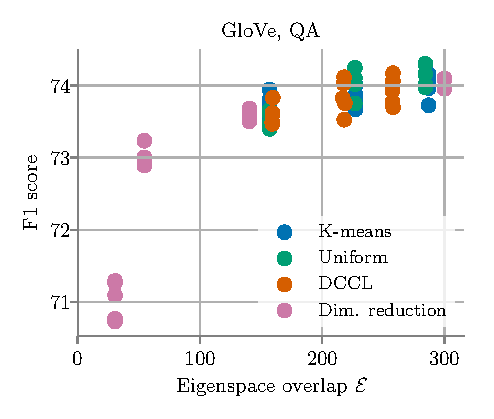
\includegraphics[width=.245\linewidth]{figures/glove400k_qa_best-f1_vs_subspace-eig-overlap_linx.pdf} &
%		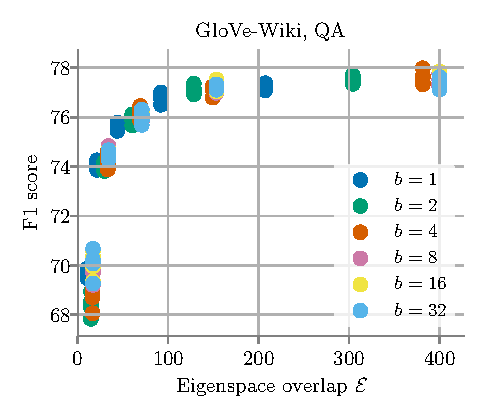
\includegraphics[width=.245\linewidth]{figures/glove-wiki400k-am_qa_best-f1_vs_subspace-eig-overlap_linx.pdf} &
%		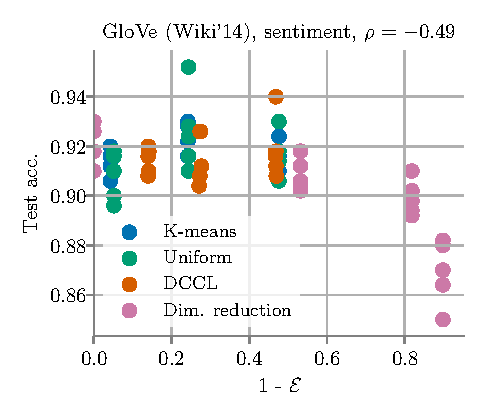
\includegraphics[width=.245\linewidth]{figures/glove400k_sentiment_trec_test-acc_vs_subspace-eig-overlap_linx.pdf} &
%		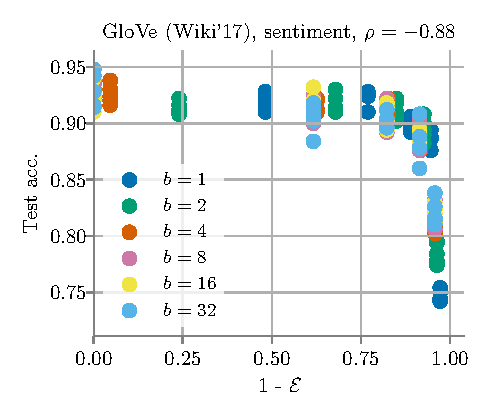
\includegraphics[width=.245\linewidth]{figures/glove-wiki400k-am_sentiment_trec_test-acc_vs_subspace-eig-overlap_linx.pdf}	\\
%		(a) GloVe (Wiki'14), QA & \;\;\;\;(b) GloVe (Wiki'17), QA  & \;\;\;\;\;\;(c) GloVe (Wiki'14), sentiment & \;\;\;\;\;(d) GloVe (Wiki'14)
%	\end{tabular}
%	\caption{Our proposed compression quality metric eigenspace overlap correlates strongly with the downstream task performance of compressed embeddings.  On both the question answering and sentiment analysis task, we demonstrate that eigenspace overlap consistently achieves strong correlation 1) across different compression methods (shown in (a), (c)) and 2) across different precision for the uniform quantization methods (shown in (b), (d)). In other words, embeddings compressed by different methods using different configurations can performs similarly in downstream tasks, when they have similar eigenspace overlap with the same reference uncompressed embedding.}
%	\label{fig:good_correlation}
%\end{figure*}

%\begin{figure*}
%	\footnotesize
%	\begin{tabular}{@{\hskip -0.0in}c@{\hskip -0.0in}c@{\hskip -0.0in}c@{\hskip -0.0in}c@{\hskip -0.0in}}
%		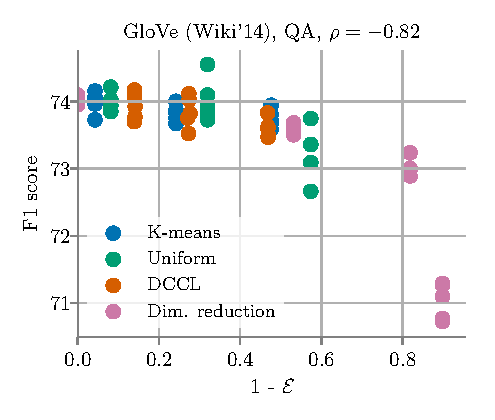
\includegraphics[width=.245\linewidth]{figures/glove400k_qa_best-f1_vs_subspace-dist-normalized_linx_stoc.pdf} &
%		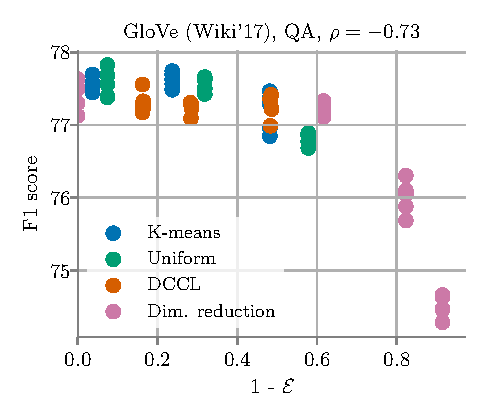
\includegraphics[width=.245\linewidth]{figures/glove-wiki400k-am_qa_best-f1_vs_subspace-dist-normalized_linx_stoc.pdf} &
%		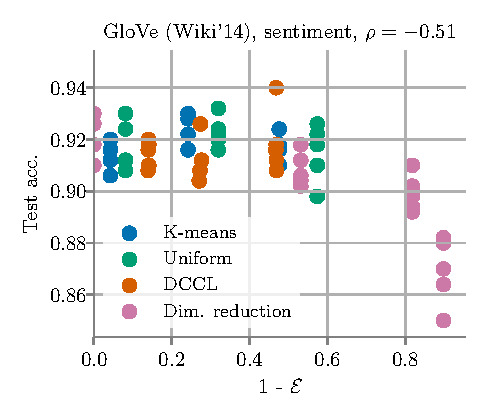
\includegraphics[width=.245\linewidth]{figures/glove400k_sentiment_trec_test-acc_vs_subspace-dist-normalized_linx_stoc.pdf} &
%		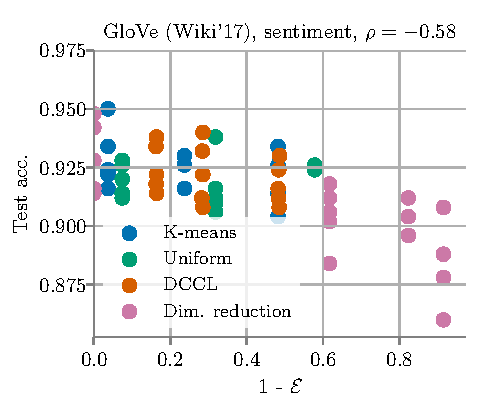
\includegraphics[width=.245\linewidth]{figures/glove-wiki400k-am_sentiment_trec_test-acc_vs_subspace-dist-normalized_linx_stoc.pdf}	\\
%		(a) GloVe (Wiki'14), QA & \;\;\;\;(b) GloVe (Wiki'17), QA  & \;\;\;\;\;\;(c) GloVe (Wiki'14), sentiment & \;\;\;\;\;(d) GloVe (Wiki'14)
%	\end{tabular}
%	\caption{\textbf{Stochastic.} Our proposed compression quality metric eigenspace overlap correlates strongly with the downstream task performance of compressed embeddings.  On both the question answering and sentiment analysis task, we demonstrate that eigenspace overlap consistently achieves strong correlation 1) across different compression methods (shown in (a), (c)) and 2) across different precision for the uniform quantization methods (shown in (b), (d)). In other words, embeddings compressed by different methods using different configurations can performs similarly in downstream tasks, when they have similar eigenspace overlap with the same reference uncompressed embedding.}
%	\label{fig:good_correlation_stoc}
%\end{figure*}

\begin{figure*}
	\footnotesize
	\begin{tabular}{@{\hskip -0.0in}c@{\hskip -0.0in}c@{\hskip -0.0in}c@{\hskip -0.0in}c@{\hskip -0.0in}}
		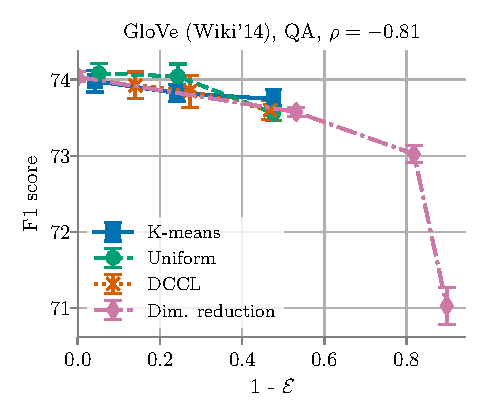
\includegraphics[width=.245\linewidth]{figures/glove400k_qa_best-f1_vs_subspace-dist-normalized_linx_det.pdf} &
		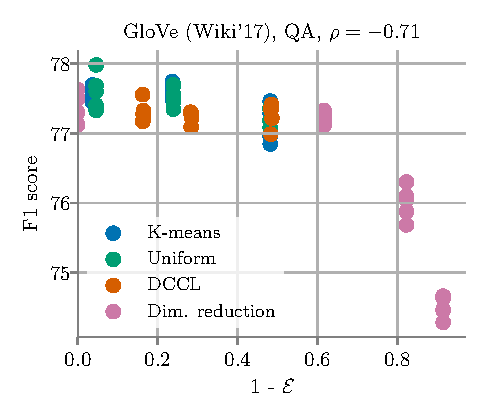
\includegraphics[width=.245\linewidth]{figures/glove-wiki400k-am_qa_best-f1_vs_subspace-dist-normalized_linx_det.pdf} &
		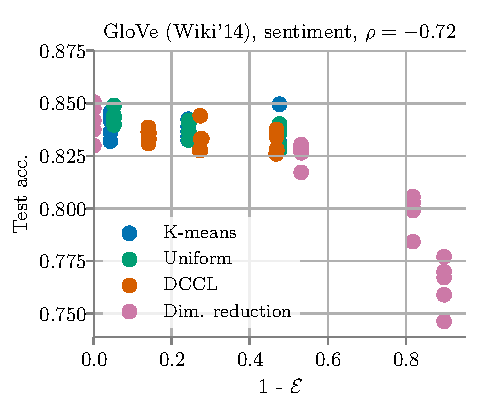
\includegraphics[width=.245\linewidth]{figures/glove400k_sentiment_sst_test-acc_vs_subspace-dist-normalized_linx_det.pdf} &
		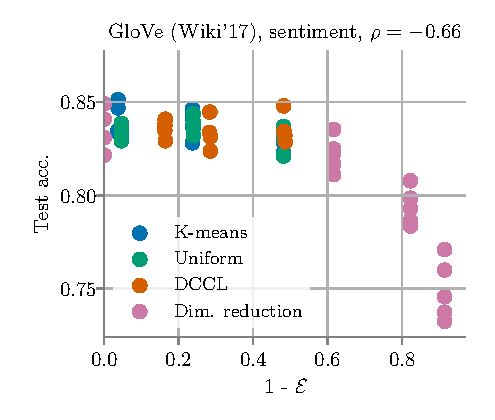
\includegraphics[width=.245\linewidth]{figures/glove-wiki400k-am_sentiment_sst_test-acc_vs_subspace-dist-normalized_linx_det.pdf}	\\
		(a) GloVe (Wiki'14), QA & \;\;\;\;(b) GloVe (Wiki'17), QA  & \;\;\;\;\;\;(c) GloVe (Wiki'14), sentiment & \;\;\;\;\;(d) GloVe (Wiki'17), 
	\end{tabular}
	\caption{Our proposed compression quality metric eigenspace overlap correlates strongly with the downstream task performance of compressed embeddings.  On both the question answering and sentiment analysis task, we demonstrate that eigenspace overlap consistently achieves strong correlation 1) across different compression methods (shown in (a), (c)) and 2) across different precision for the uniform quantization methods (shown in (b), (d)). In other words, embeddings compressed by different methods using different configurations can performs similarly in downstream tasks, when they have similar eigenspace overlap with the same reference uncompressed embedding.}
	\label{fig:good_correlation_det}
\end{figure*}


%\begin{figure*}
%	\footnotesize
%	\begin{tabular}{@{\hskip -0.0in}c@{\hskip -0.0in}c@{\hskip -0.0in}c@{\hskip -0.0in}}
%		\includegraphics[width=.245\linewidth]{figures/glove400k_translation_BLEU4_vs_subspace-dist-normalized_linx_stoc.pdf} &
%		\includegraphics[width=.245\linewidth]{figures/glove-wiki400k-am_translation_BLEU4_vs_subspace-dist-normalized_linx_stoc.pdf} &
%		\includegraphics[width=.245\linewidth]{figures/glove-wiki400k-am_translation_BLEU4_vs_subspace-dist-normalized_linx_stoc.pdf}	\\
%		\includegraphics[width=.245\linewidth]{figures/glove400k_translation_min_val_loss_vs_subspace-dist-normalized_linx_stoc.pdf} &
%		\includegraphics[width=.245\linewidth]{figures/glove-wiki400k-am_translation_min_val_loss_vs_subspace-dist-normalized_linx_stoc.pdf} &
%		\includegraphics[width=.245\linewidth]{figures/glove-wiki400k-am_translation_min_val_loss_vs_subspace-dist-normalized_linx_stoc.pdf}	\\
%		\includegraphics[width=.245\linewidth]{figures/glove400k_translation_min_val_ppl_vs_subspace-dist-normalized_linx_stoc.pdf} &
%		\includegraphics[width=.245\linewidth]{figures/glove-wiki400k-am_translation_min_val_ppl_vs_subspace-dist-normalized_linx_stoc.pdf} &
%		\includegraphics[width=.245\linewidth]{figures/glove-wiki400k-am_translation_min_val_ppl_vs_subspace-dist-normalized_linx_stoc.pdf}	\\
%		(a) GloVe (Wiki'14), translation & \;\;\;\;(b) GloVe (Wiki'17), translation  & \;\;\;\;\;\;(c) FastText, translation 	\end{tabular}
%	\caption{\textbf{Stochastic translation only. First Row, BLUE4; Second Row, val. loss; Third Row, val. perp} }
%	\label{fig:good_correlation_stoc_trans_only}
%\end{figure*}

%\begin{figure*}
%	\footnotesize
%	\begin{tabular}{@{\hskip -0.0in}c@{\hskip -0.0in}c@{\hskip -0.0in}c@{\hskip -0.0in}}
%		\includegraphics[width=.245\linewidth]{figures/glove400k_translation_BLEU4_vs_subspace-dist-normalized_linx_det.pdf} &
%		\includegraphics[width=.245\linewidth]{figures/glove-wiki400k-am_translation_BLEU4_vs_subspace-dist-normalized_linx_det.pdf} &
%		\includegraphics[width=.245\linewidth]{figures/glove-wiki400k-am_translation_BLEU4_vs_subspace-dist-normalized_linx_det.pdf}	\\
%		\includegraphics[width=.245\linewidth]{figures/glove400k_translation_min_val_loss_vs_subspace-dist-normalized_linx_det.pdf} &
%		\includegraphics[width=.245\linewidth]{figures/glove-wiki400k-am_translation_min_val_loss_vs_subspace-dist-normalized_linx_det.pdf} &
%		\includegraphics[width=.245\linewidth]{figures/glove-wiki400k-am_translation_min_val_loss_vs_subspace-dist-normalized_linx_det.pdf}	\\
%		\includegraphics[width=.245\linewidth]{figures/glove400k_translation_min_val_ppl_vs_subspace-dist-normalized_linx_det.pdf} &
%		\includegraphics[width=.245\linewidth]{figures/glove-wiki400k-am_translation_min_val_ppl_vs_subspace-dist-normalized_linx_det.pdf} &
%		\includegraphics[width=.245\linewidth]{figures/glove-wiki400k-am_translation_min_val_ppl_vs_subspace-dist-normalized_linx_det.pdf}	\\
%		(a) GloVe (Wiki'14), translation & \;\;\;\;(b) GloVe (Wiki'17), translation  & \;\;\;\;\;\;(c) FastText, translation 	\end{tabular}
%	\caption{\textbf{Deterministic translation only. First Row, BLUE4; Second Row, val. loss; Third Row, val. perp} }
%	\label{fig:good_correlation_stoc_trans_only}
%\end{figure*}

In this section, we introduce the \textit{eigenspace overlap metric} to measure the quality of a compressed embedding relative to the uncompressed embedding.
We prove average-case generalization bounds for this metric in the context of linear regression, and show that this metric indeed aligns very well with the downstream performance of the compressed embeddings.

\subsection{Eigenspace Overlap and Generalization}
\label{subsec:eigen_overlap}
\begin{definition}
Given two embedding matrices $X \in \RR^{n \times d}$, $\tX \in \RR^{n \times k}$, whose Gram matrices have eigendecompositions $XX^T = USU^T$, $\tX\tX^T = VRV^T$ for $U \in \RR^{n\times d}$, $V\in \RR^{n \times k}$, we define the eigenspace overlap metric $\eigover(X,\tX) \defeq  \frac{1}{\max(d,k)}\|U^T V\|_F^2$.
\end{definition}

This metric measures the degree to which the span of the eigenvectors with nonzero eigenvalue of $\tX\tX^T$ agrees with that of $XX^T$.
In particular, assuming $k\leq d$, it measures the ratio between the squared Frobenius norm of $U$ before and after being projected onto $V$.
As an example, if the span $\Span(V)$ of the columns of $V$ is a subspace of $\Span(U)$, then $\eigover(X,\tX) = \frac{1}{d}\|U^T V\|_F^2 = \frac{1}{d}\|UU^T V\|_F^2 = \frac{1}{d}\|V\|_F^2 = \frac{k}{d}$.
In contrast, if $\Span(V)$ is orthogonal to $\Span(U)$, then $\eigover(X,\tX) = 0$.

We now show that this metric is closely related to the generalization performance of the linear regression model trained using the compressed embeddings $\tX$ in place of $X$.
For simplicity, we will consider here the noiseless fixed design regression setting;
In this setting, the training loss is equal to the generalization loss.
Letting $y\in\RR^n$ denote the vector of labels and using the closed form solution for the optimal parameters $w^* = (X^T X)^{-1}X^Ty$, we can derive that the generalization performance is equal to $\cR(X) = \|Xw^* - y\|^2 = \|y\|^2 - \|U^T y\|^2$.

To expose the influence of the eigenspace overlap on the generalization performance, it will be necessary for us to considering an average-case analysis.
This is necessary because in worst-case analysis, if there exists a single direction in $\Span(U)$ orthogonal to $\Span(V)$ (which always occurs when $\dim(V) < \dim(U)$) the label vector $y$ can simply be equal to this direction.
In this case $\cR(X) = \|y\|^2 - \|U^T y\|^2 = 0$, while $\cR(\tX) = \|y\|^2 - \|V^T y\|^2 = \|y\|^2$.
Thus, the setting we will consider instead is one where $y$ is a random vector in $\Span(U)$.
We consider the setting $y \in \Span(U)$ (which implies $\cR(X) = 0$) for simplicity because we are most interested in the situation where we know the uncompressed embedding matrix $X$ performs well, and we would like to understand how well $\tX$ will do.
We now present our average-case result (see Appendix~\ref{app:theory} for proof):

\begin{proposition}
If $y = Uz$ for a random vector $z \in \RR^d$ with zero mean and identity covariance, then
\begin{eqnarray}
\expect{y}{\cR(\tX) - \cR(X)} &=& d\cdot(1 - \eigover(X,\tX))
\end{eqnarray}
\end{proposition}

This proposition reveals that a larger eigenspace overlap value results in better generalization performance for the compressed embedding.

\paragraph{Discussion}
Here, we provide a more detailed discussion of two important aspects of the eigenspace overlap metric:
(1) It only depends on the left singular vectors of the embedding matrices;
(2) It is much more robust than the previously proposed metrics to perturbations of the embedding matrix which are unlikely to significantly change the generalization performance (in the average-case sense).

To better understand why the eigenspace overlap only depends on the left singular vectors of the embedding matrices, we first observe in the above equation for $\cR(X)$ that the generalization performance of a linear model trained on $X$ only depends on the left singular vectors of $X$ (assuming $X$ is full-rank).
To see why this is the case, consider the predicted labels $y \defeq Xw$, for some linear model $w \in \RR^d$ over $X$.
If we replace $X$ with $\tX \defeq U \tSigma \tW^T$, and we replace $w$ with $\tw \defeq \tW \tSigma^{-1} \Sigma W^T w$, then $\tX \tw = U\tSigma \tW^T \tW \tSigma^{-1} \Sigma W^T w = Xw$.
Thus, a linear model over $\tX$ can exactly replicate the output of any linear model over $X$, assuming the left singular vectors of $X$ and $\tX$ are equal.
This observation provides intuition for why it is reasonable for the eigenspace overlap metric to only consider the left singular vectors of the embedding matrices.

To demonstrate the robustness of the eigenspace overlap to perturbations of the embedding matrix unlikely to have a large effect on generalization performance, we consider the following simple perturbation:
if $X = \sum_{i=1}^{d} \sigma_i U_i W_i^T$ is the singular value decomposition of $X$, we consider setting it's largest eigenvalue to 0, resulting in the perturbed matrix $\tX \defeq \sum_{i=2}^{d} \sigma_i U_i W_i^T$.
Assuming a linear model $y = Xw = \sum_i \alpha_i U_i$, $\tX$ would have a generalization error of $\alpha_1^2$.
If we assume that $\alpha_1^2 \ll \sum_{i=1}^{d-1}\alpha_i^2$ (as is the case in our average-case analysis), then $\tX$ would perform similarly to $X$.

In Table~\ref{table:perturb}, we show the impact of the above perturbation on the various metrics we have discussed for comparing embedding matrices.
At a high-level, we observe that this perturbation can have a dramatic effect of the previously proposed metrics, while having minimal effect on the eigenspace overlap metric.
For example, the $\Delta_1$ metric is very sensitive to setting the largest singular value of an embedding to 0.
This makes sense, because $\Delta_1$ can be used to attain a worst-case generalization bound for the perturbed embeddings \citep{lprff18}, and there exist cases where setting the smallest singular value to 0 can significantly harm the generalization performance of the embeddings (\eg, if $\alpha_d^2 \approx \|\alpha\|^2$).
Thus, while the $\Delta_1$ metric is an important metric for understanding the worst-case performance of the compressed embeddings, it is generally an overly pessimistic metric.
Our metric, on the other hand, is generally unable to provide worst-case guarantees, but aligns nicely with the expected performance of the compressed embeddings in the average-case setting.

Another perturbation which can affect the other metrics much more than it affects the eigenspace overlap metric is right-multiplication by an invertible matrix.
While this perturbation can have unbounded effects on the other metrics, it has no effect on the eigenspace overlap metric, and no effect on generalization performance.
%Note that the eigenspace overlap metric is additionally invariant to right multiplication of the embedding matrix by any invertible matrix, while none of the other metrics are.

\begin{table}
	\caption{In this table, we consider the effect of perturbing an embedding matrix $X$ by setting its largest singular value to 0 on the various compression quality metrics discussed above.
%	In the last row, we plot the generalization error $\cR(\tX) = \|\tX \tw - y\|^2$ which results from learning a linear model on top of $\tX_1$ or $\tX_2$ in place of $X$, where we assume the labels $y = \sum_{i=1}^d \alpha_i U_i$.}
	As we can see, setting the largest singular value of $X$ to 0 can have a disproportionately large effect on the relative reconstruction error, relative PIP loss, and $\Delta_1$ metrics (values can approach 1), while having a modest effect on the eigenspace overlap metric (value of $1/d$ always).
%	In the last row, we plot the generalization error $\cR(\tX) = \|\tX \tw - y\|^2$ which results from learning a linear model on top of the perturbed embeddings in place of $X$, where we assume the labels $y = \sum_{i=1}^d \alpha_i U_i$.
%	If we assume that $\alpha_1^2 \ll \sum_{i=1}^{d-1}\alpha_i^2$ (as in our average-case analysis), then the perturbed embeddings would perform similarly to the unperturbed embeddings.
}
	\centering
	\begin{tabular}{ c | c }
		Compression quality metric & Metric after perturbation \\ \midrule
		Rel. reconstruction error &  $\sigma_1/\sqrt{\sum_{i=1}^d \sigma_i^2}$ \\
		Rel. PIP loss & $\sigma_1^2 / \sqrt{\sum_{i=1}^d \sigma_i^4}$ \\
		$\Delta_1$ & $\sigma_1^2 / \Big(\sigma_1^2 + \lambda\Big)$ \\
		$\Delta_2$ & 0 \\
		$1-\eigover(X,\tX)$ & $\frac{1}{d}$\\ %\hline
%		$\cR(\tX)$ & $\alpha_1^2$\\
	\end{tabular}
	\label{table:perturb}
\end{table}

%\begin{table}
%	\caption{In this table, we consider two perturbations $\tX_1$ and $\tX_2$ of $X$, and compute the value of the various metrics of compression quality between these perturbations and $X$. Specifically, we consider $\tX_1 = aX$ for some $a \geq 0$, and $\tX_2 = \sum_{i=1}^{d-1} \sigma_i U_i W_i^T$, where $X = \sum_{i=1}^d \sigma_i U_i W_i^T$.  We let $\sigma_{\min}$ and $\sigma_{\max}$ denotes the smallest and largest singular values of $X$, respectively. In the last row, we plot the generalization error $\cR(\tX) = \|\tX \tw - y\|^2$ which results from learning a linear model on top of $\tX_1$ or $\tX_2$ in place of $X$, where we assume the labels $y = \sum_{i=1}^d \alpha_i U_i$.}
%	\centering
%	\begin{tabular}{ c | c | c }
%		& $\tX_1$ & $\tX_2$ \\ \hline
%		Rel. reconstruction error & $|a-1| \cdot \|X\|_F$ & $\sigma_{\min}$ \\
%		Rel. PIP loss & $|a^2 - 1| \cdot \|XX^T\|_F$ & $\sigma_{\min}^2$ \\
%		$\Delta_1$ & $\max\Big(0,\frac{\sigma_{\max}^2 (1-a^2) }{\sigma_{\max}^2 + \lambda}\Big)$ & $\frac{\sigma_{\min}^2}{\sigma_{\min}^2 + \lambda}$ \\
%		$\Delta_2$ & $\max\Big(0,\frac{\sigma_{\max}^2 (a^2-1) }{\sigma_{\max}^2 + \lambda}\Big)$ & 0 \\
%		$1-\eigover(X,\tX)$ & $0$ & $\frac{1}{d}$\\ \hline
%		$\cR(\tX)$ & $0$ & $\alpha_d^2$\\
%	\end{tabular}
%\label{table:perturb}
%\end{table}

\subsection{Revisiting the Performance of Compressed Embeddings}
\label{subsec:revisit}
We now demonstrate that unlike the metrics we discussed in Section~\ref{sec:prelim}, this metric empirically aligns very well with the performance of compressed embeddings on downstream tasks.
In Figure~\ref{fig:good_correlation} we show scatter plots of downstream performance vs.\ eigenspace overlap, and see that in general higher eigenspace overlap corresponds to better performance.
Thus, even though our analysis is for a linear regression setting, we can see that this metric predicts performance well on a variety of downstream tasks which use neural networks for training.
%\todo{Discuss performance relative to $\Delta_1$,$\Delta_2$?}


\section{Uniform Quantization for Word Embeddings}
\label{sec:quant_embed}
To further demonstrate how the eigenspace overlap metric can be used to better understand the performance of compressed embeddings, in this section we show that we can upper bound the eigenspace overlap for uniformly quantized embeddings.
Given the above theoretical and empirical connections between eigenspace overlap and generalization performance, these bounds help explain why the uniformly quantized embeddings perform so well.
To prove these bounds, we leverage the classic Davis-Kahan $\sin(\Theta)$ theorem from matrix perturbation analysis \citep{sintheta70}.
Because we know exactly what the noise structure of the uniform quantization method is, we can use this knowledge to bound how much the eigenspace of the compressed embeddings can differ from the uncompressed embeddings.

We now present the result (see Appendix~\ref{app:theory} for proof):
\begin{theorem}
	Let $X \in \RR^{n\times d}$ be a bounded embedding matrix with $X_{ij} \in [-\frac{1}{\sqrt{d}},\frac{1}{\sqrt{d}}]$ with largest and smallest singular values $\sigma_{\max}$ and $\sigma_{\min}$.
	Then the eigenspace overlap of the corresponding $b$-bit uniformly quantized embedding matrix can be lower bounded as follows:
	\begin{eqnarray*}
		\eigover(X,\tX) &\geq& 1 - \Bigg(\frac{4\sqrt{n}}{\sqrt{d}(2^b-1)} \cdot \frac{\sigma_{\max} + \frac{\sqrt{n}}{2^b-1} }{\sqrt{\sigma_{\min}}} \Bigg)^2
	\end{eqnarray*}
\label{thm1}
\end{theorem}

We can further simplify this expression using the fact that $\sigma_{\max} = \|X\|_2 \leq \sqrt{n}$; using this fact, we get the following corollary:
\begin{corollary}
If $b \geq \log_2\bigg(\frac{8n}{\sqrt{\rho \, d\, \sigma_{\min}}} + 1\bigg)$, then the $b$-bit uniformly quantized embedding matrix $\tX$ satisfies $\eigover(X,\tX) \geq 1-\rho$.
\end{corollary}

The corollary shows that one can attain an eigenspace overlap arbitrarily close to $1$ if a sufficient number of bits $b$ are used.

\paragraph{Empirical Validation of Theory}
We now validate the above theory by showing how the eigenspace overlap grows as the precision of the uniformly quantized embeddings is increased.
For this experiment, we generate a random matrix $X \in \RR^{10^5 \times 300}$, with each entry drawn uniformly at random in the interval $[-\frac{1}{\sqrt{300}}, \frac{1}{\sqrt{300}}]$.
We then measure the eigenspace overlap of quantized versions of $X$, for precisions $b \in \{1,2,4,8,16,32\}$.
As we can see in Figure~\ref{fig:micro_eigoverlap_vs_prec}, the eigenspace overlap grows quite quickly as the precision grows, attaining a value of approximately $0.82$ at $b=2$, and $0.99$ at $b=4$.
This helps explain the strong empirical performance of the uniformly quantized embeddings which we observed at low precisions on the real word embedding experiments (Figure~\ref{fig:perf_comp}).

%\todo{Add section on clippings effect on the eigenspace overlap?}

\begin{figure}
	\begin{tabular}{c}
		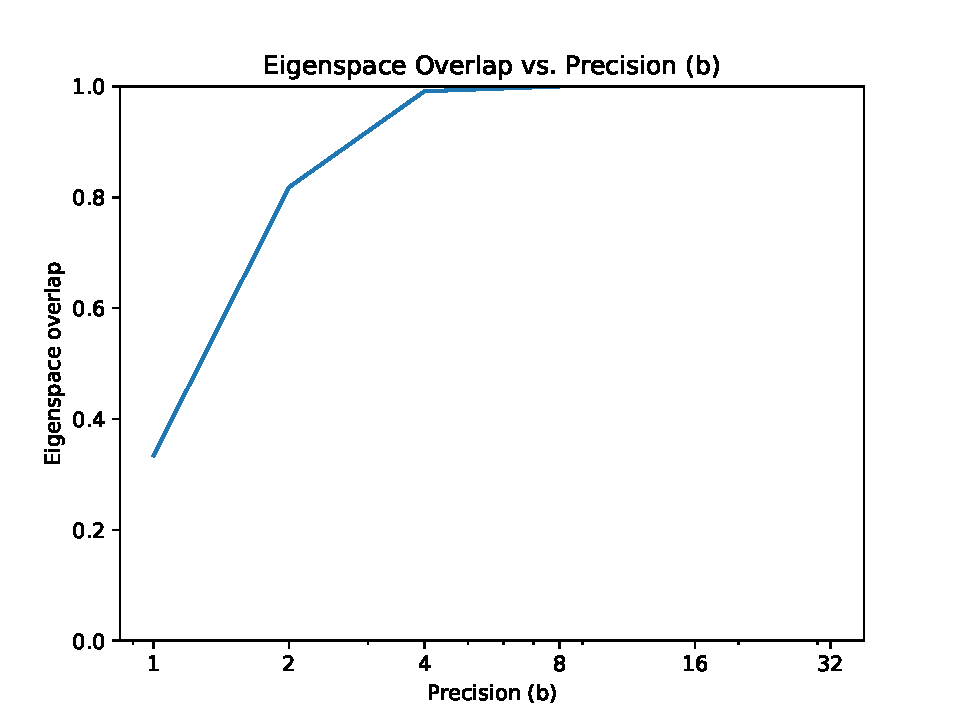
\includegraphics[width=\linewidth]{figures/micro_eig_overlap_vs_precision.pdf} 
\end{tabular}
\caption{Empirical Validation of Theorem~\ref{thm1}. We measure the eigenspace overlap of uniformly quantized embeddings with the uncompressed embedding for various precisions ($b\in\{1,2,4,8,16,32\}$), and observe the eigenspace overlap grows quickly as the precision grows.  For the uncompressed embedding, we generate a random matrix $X \in \RR^{10^5 \times 300}$, with each entry drawn uniformly at random in $[-\frac{1}{\sqrt{300}}, \frac{1}{\sqrt{300}}]$.}
\label{fig:micro_eigoverlap_vs_prec}
\end{figure}

%\subsection{Theory validation}
%	\begin{itemize}
%		\item Impact of quantization on overlap 
%			\begin{itemize}
% 				\item Exp 1: overlap vs precision for different dimensionality. Expectation: overlap increases with higher precision.
%				\item Exp2: overlap vs dimensionality for different precision. Expectation: overlap increases with dimensionality. This explains that under fix memory budget, using lower bits quantization can be beneficial
%			\end{itemize}
%		\item The impact of clipping on eigen-subspace overlap
%			\begin{itemize}
%				\item Simulation based experiments on subspace overlap as a function of different clipping threshold and precision. 
%				\item The way we introduce this in: in our main theorem, we assume the dynamic range is $O(1/\sqrt{d})$ as a consequence of the automatic clipping. We want to show here this is the case in practice and then discuss the specific way clipping influence eigenspace overlap.
%			\end{itemize}
%		\item Loop-back discussion on the large scale empirical experiments in Section~\ref{subsec:hard_explain}
%	\end{itemize}


\section{Experiments}
\label{sec:exp}
We now evaluate the performance of our word embedding compression algorithm on a variety of NLP tasks and embeddings types.
We show that our compression method is consistently able to match the performance of more complex baselines (DCCL, k-means), while dramatically outperforming more naive baselines (dimensionality reduction).
We additionally present results in which we maintain the memory budget fixed by  jointly varying the dimension and precision of the compressed embeddings;
we observe that in this memory-constrained setting, the best compressed embeddings attain \todo{XX\%} to \todo{YY\%} better performance than the full-precision embeddings.
This demonstrates the importance of considering low-precision when trying to attain the best possible performance under a memory budget.

\subsection{Large-scale evaluation}
\begin{itemize}
	\item \textbf{Embeddings}: GloVe ($d\in\{50,100,200,300\}$, $n=400k$) and fastText ($d=300$, $n=10^6$) pre-trained.
	\item \textbf{Baselines}: k-means, DCCL, dim. reduction (GloVe)
	\item \textbf{Tasks}: DrQA, sentiment, intrinsics, synthetics.
	\item \textbf{Compression ratios}: 8x-32x.
	\item \textbf{Number of random seeds}: 5
\end{itemize}

In Figure~\ref{fig:drqa_sent_results} we show that on both question answering and sentiment analysis tasks the uniform quantization method performs comparably to k-means and DCCL, while performing significantly better than the dimensionality reduction baseline.

%\begin{figure}
%\begin{center}
%\centerline{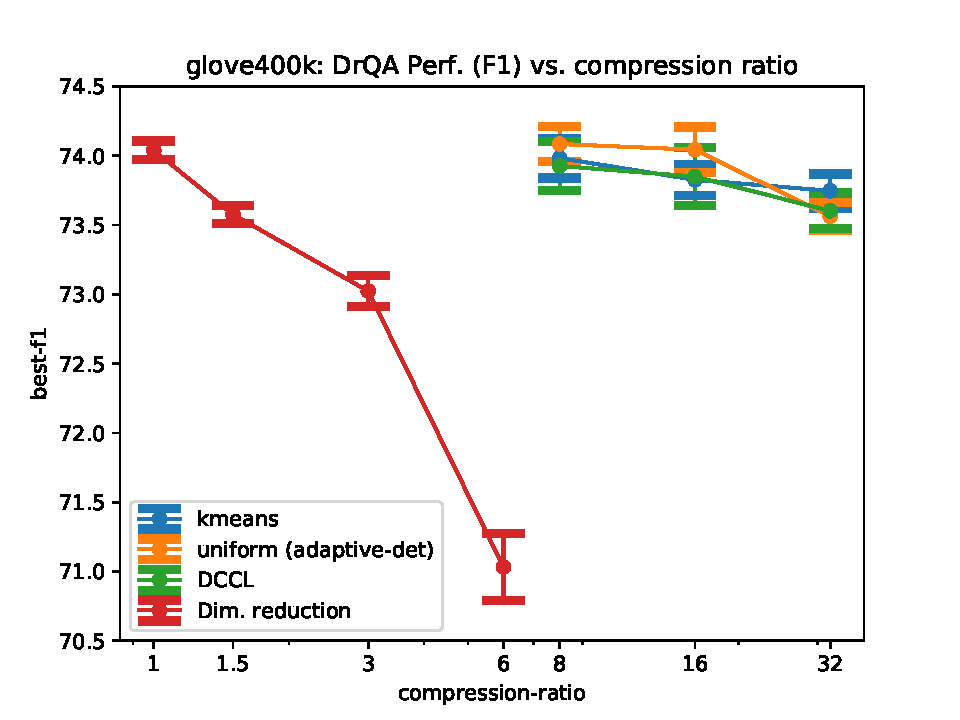
\includegraphics[width=\columnwidth]{figures/glove400k_drqa_vs_compression.pdf}}
%\caption{Question answering performance (DrQA) for a number of compression methods at various compression ratios, on pre-trained GloVe embedding.  Uniform quantization performs similarly to k-means and DCCL, while significantly outperforming the dimensionality reduction baseline. \todo{TODO: Include fastText results (though there won't be a dim. reduction baseline, since they don't release pre-trained embeddings at smaller dimensions.)}}
%\label{fig:glove400k_drqa}
%\end{center}
%\end{figure}

\begin{figure*}
	\centering
	\begin{small}
		%		\begin{tabular}{c c c c}
		\begin{tabular}{@{\hskip -0.0in}c@{\hskip -0.0in}c@{\hskip -0.0in}}
			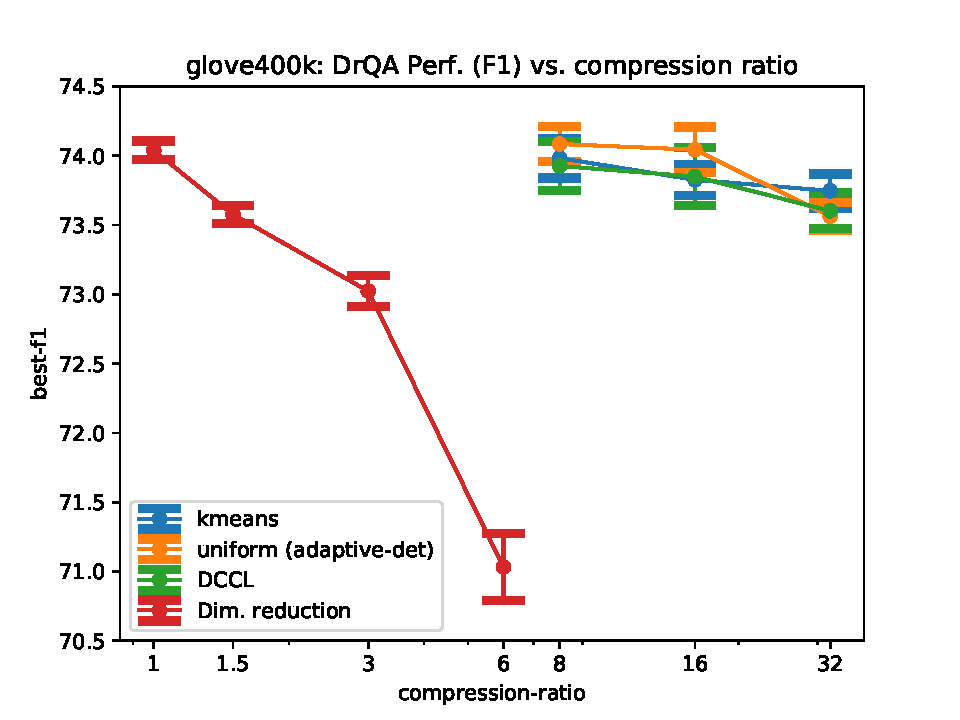
\includegraphics[width=0.4\linewidth]{figures/glove400k_drqa_vs_compression.pdf} &
			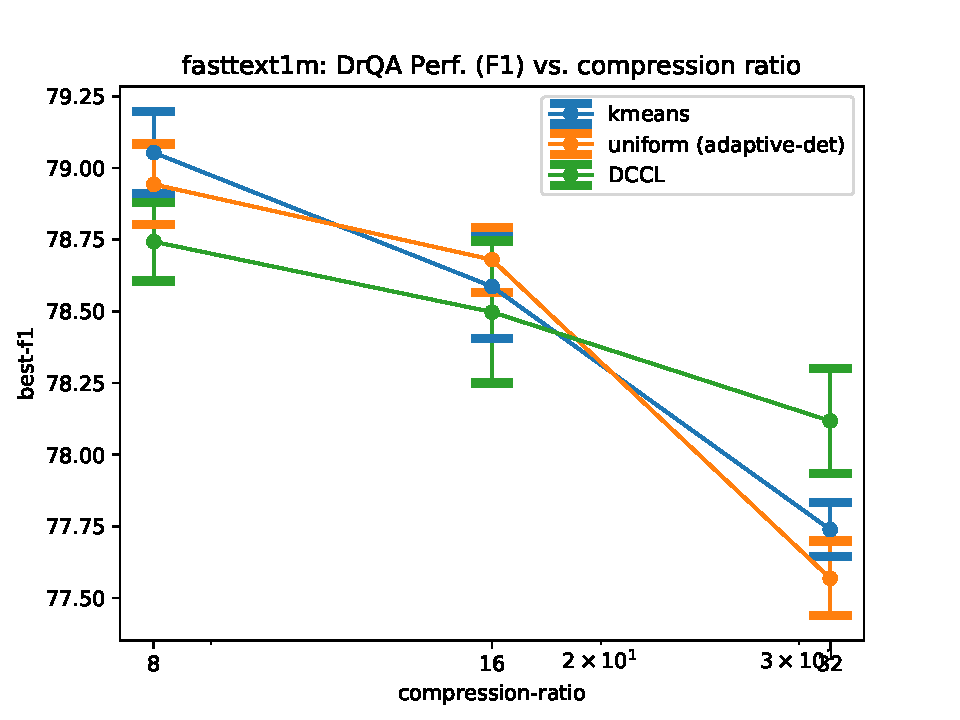
\includegraphics[width=0.4\linewidth]{figures/fasttext1m_drqa_vs_compression.pdf} \\
			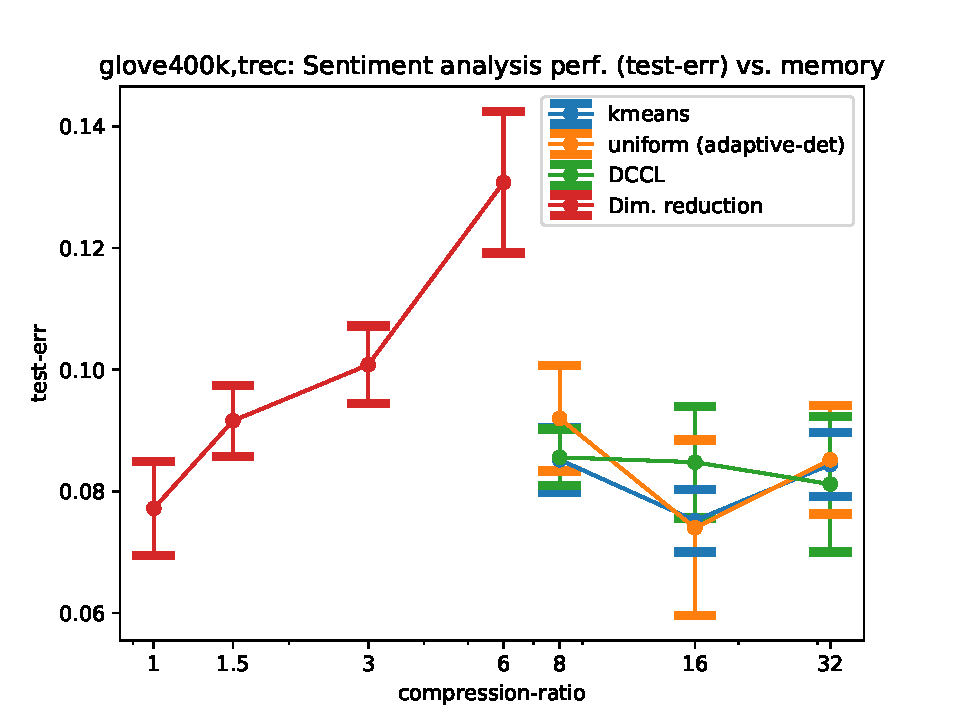
\includegraphics[width=0.4\linewidth]{figures/glove400k_trec_test-err_vs_compression.pdf} &
			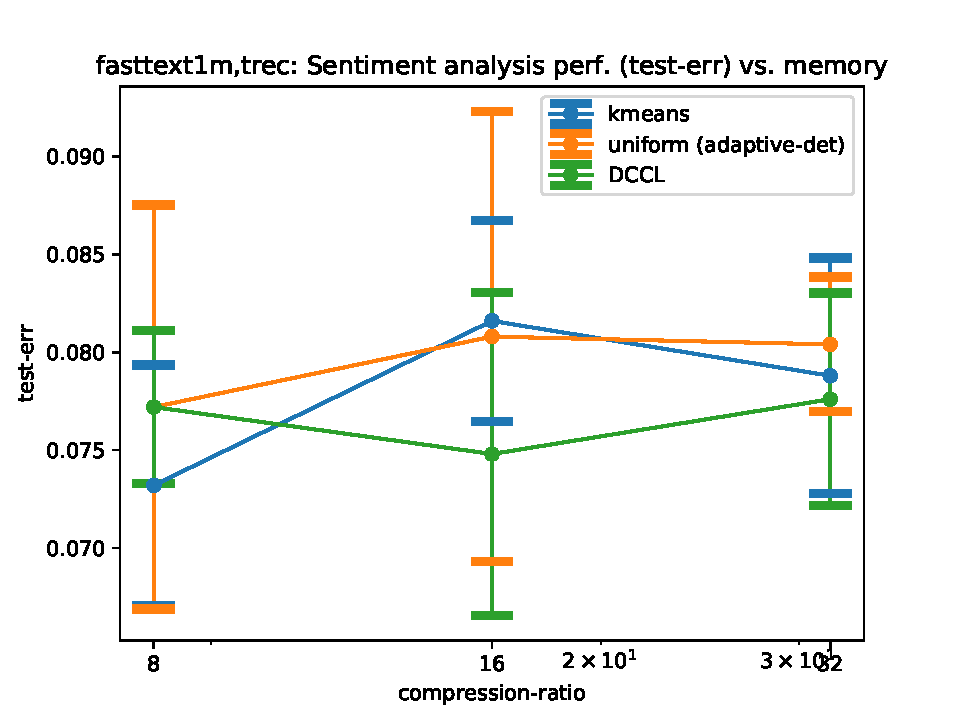
\includegraphics[width=0.4\linewidth]{figures/fasttext1m_trec_test-err_vs_compression.pdf} \\
			\;\;\;\;\;(a) & \;\;\;\;\;\;(b) 
		\end{tabular}
	\end{small}
\caption{Question answering (top) and sentiment analysis (bottom) performance for a number of compression methods at various compression ratios, on pre-trained 300-dimensional GloVe and fastText embeddings.
Uniform quantization performs similarly to k-means and DCCL.  For GloVe, we are also able to compare with pre-trained embeddings of smaller dimensions ($d\in\{50,100,200,300\}$), and observe that compressing the 300-dimensional embeddings is significantly better than using a lower dimension.}
\label{fig:drqa_sent_results}
\end{figure*}

\begin{figure*}
	\centering
	\begin{small}
		%		\begin{tabular}{c c c c}
		\begin{tabular}{@{\hskip -0.0in}c@{\hskip -0.0in}c@{\hskip -0.0in}}
			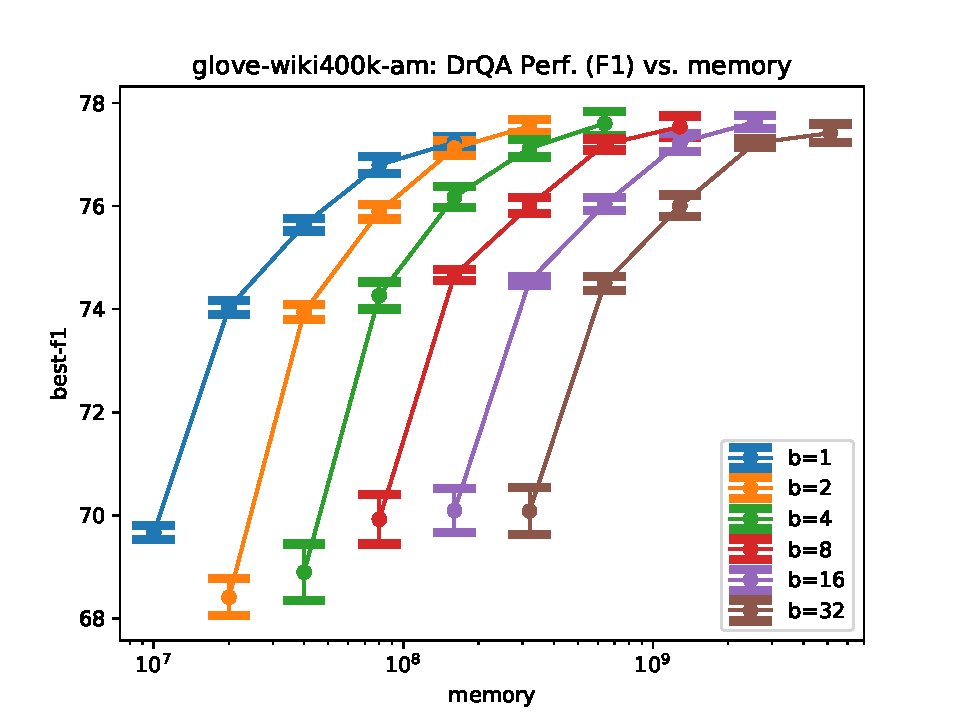
\includegraphics[width=0.4\linewidth]{figures/glove-wiki400k-am_drqa_vs_compression.pdf} &
			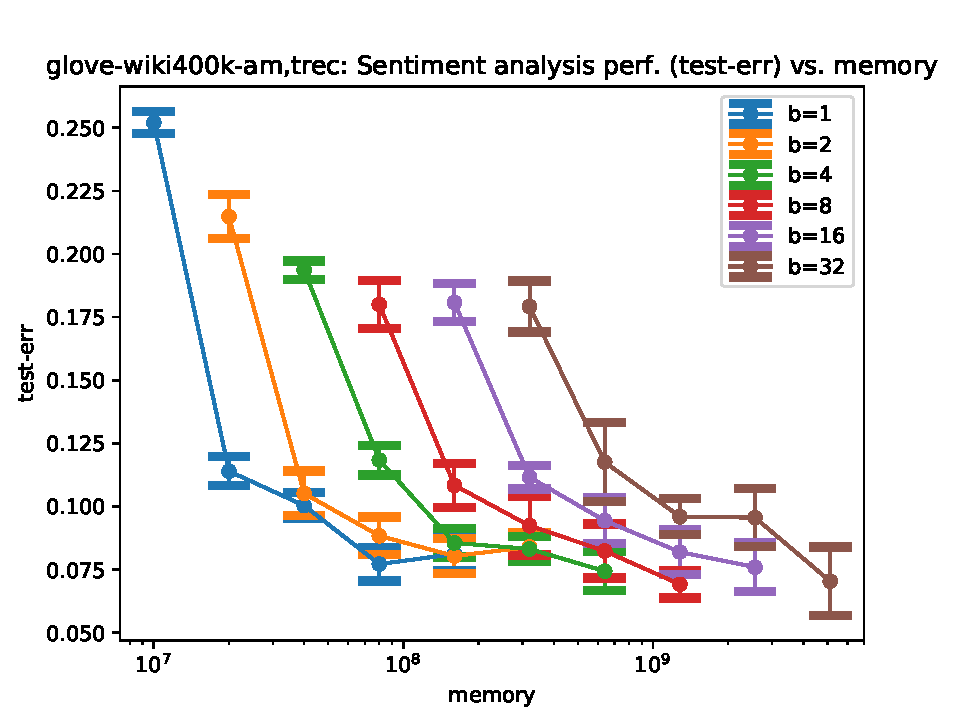
\includegraphics[width=0.4\linewidth]{figures/glove-wiki400k-am_trec_test-err_vs_compression.pdf} \\
			\;\;\;\;\;(a) & \;\;\;\;\;\;(b) 
		\end{tabular}
	\end{small}
	\caption{DrQA and sentiment analysis results (TREC dataset), where we train GloVe embeddings of various dimensions ($d\in\{25,50,100,200,400\}$) and compress them at various precisions ($b \in \{1,2,4,8,16,32\}$) with uniform quantization.  Here we see that when considering a memory budget, it is best to use low-precision features with high-dimensional embeddings.}
	\label{fig:drqa_sent_dimVsPrec}
\end{figure*}

%\begin{figure*}
%	\centering
%	\begin{small}
%		%		\begin{tabular}{c c c c}
%		\begin{tabular}{@{\hskip -0.0in}c@{\hskip -0.0in}c@{\hskip -0.0in}}
%			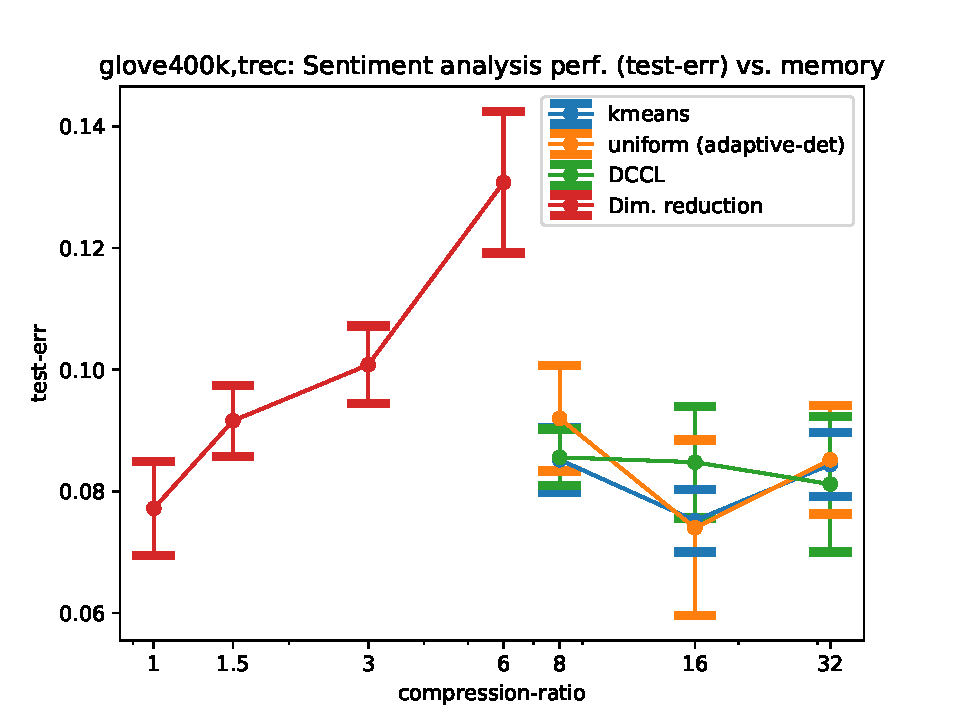
\includegraphics[width=0.45\linewidth]{figures/glove400k_trec_test-err_vs_compression.pdf} &
%			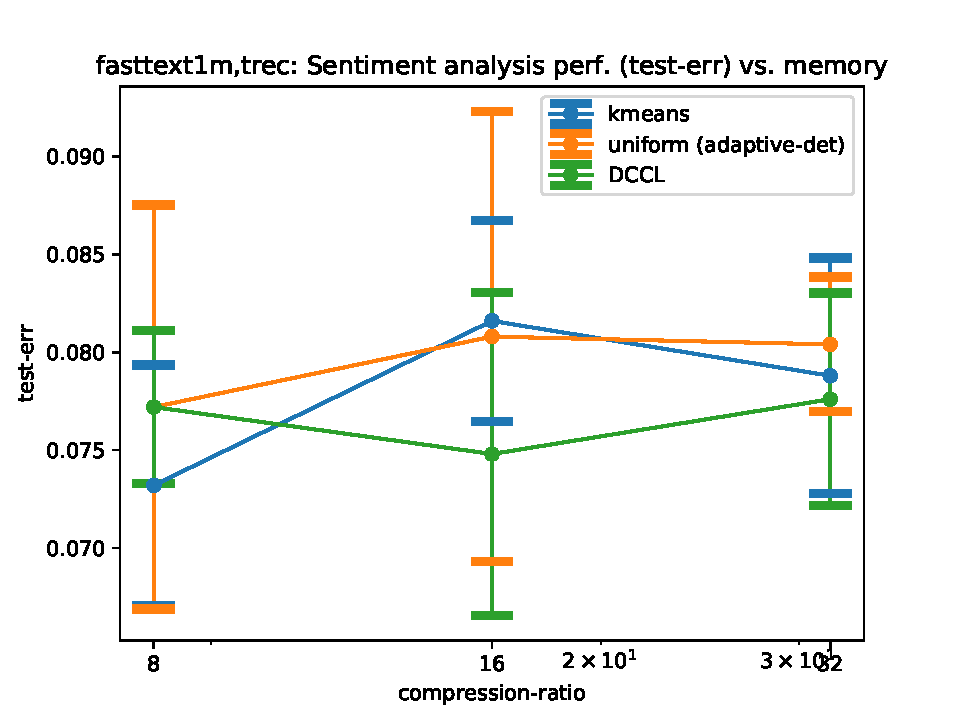
\includegraphics[width=0.45\linewidth]{figures/fasttext1m_trec_test-err_vs_compression.pdf} \\
%			\;\;\;\;\;(a) & \;\;\;\;\;\;(b) 
%		\end{tabular}
%	\end{small}
%	\caption{Sentiment analysis results (TREC dataset).}
%	\label{fig:sentiment}
%\end{figure*}

\subsection{Fixed budget experiments}
\begin{itemize}
	\item \textbf{Embeddings}: We train GloVe embeddings on a Wiki 2017 dump, for $n=400k$ and $d \in \{25,50,100,200,400,800\}$.
	\item \textbf{Bitrates}: We compress embeddings for $b \in \{1,2,4,8,16,32\}$.
	\item \textbf{Tasks}: DrQA, sentiment, intrinsics, synthetics.
	\item \textbf{Number of random seeds}: 5
\end{itemize}

In Figure~\ref{fig:drqa_sent_dimVsPrec}, we show that when considering a fixed memory budget, it is best to use low-precision and high-dimensions, on both question answering and sentiment analysis tasks.

%\begin{figure}
%	\begin{center}
%		\centerline{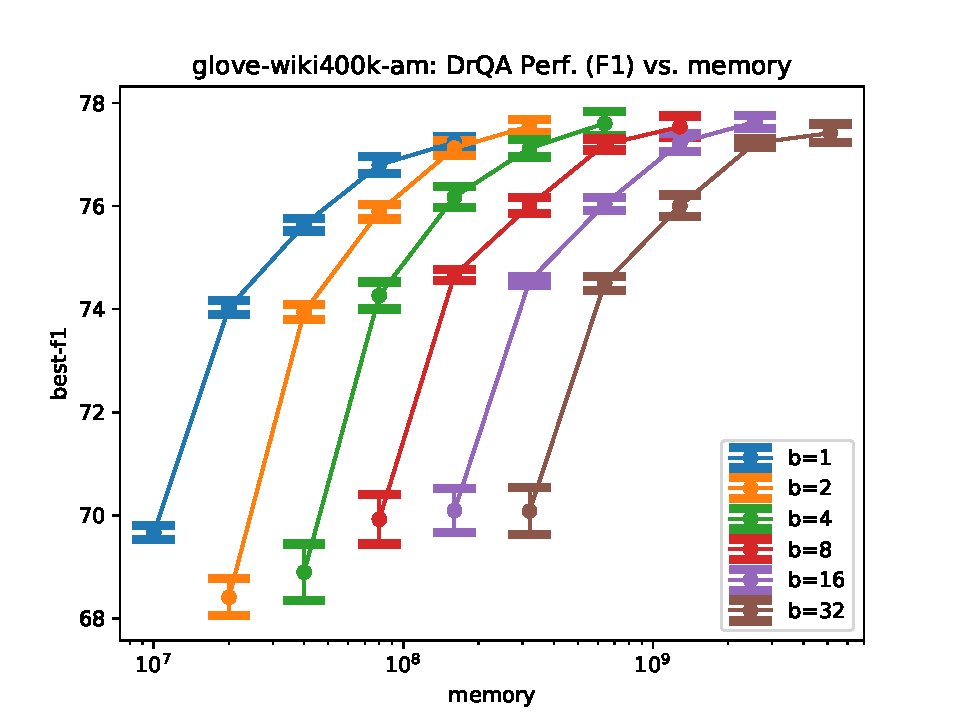
\includegraphics[width=\columnwidth]{figures/glove-wiki400k-am_drqa_vs_compression.pdf}}
%		\caption{We compress GloVe embeddings for dimensions $d\in\{25,50,100,200,400\}$ at precision values $b\in\{1,2,4,8,16,32\}$, and measure performance on question-answering (DrQA).  \todo{TODO: Include $d=800$ results, which are worse than $d=400$?}}
%		\label{fig:glove400k_dim_vs_prec}
%	\end{center}
%\end{figure}


%\section{Uniform Quantization of Word Embeddings}
%\label{sec:uniform}
%To further demonstrate how the eigenspace overlap metric can be used to better understand the performance of compressed embeddings, in this section we show that we can upper bound the eigenspace overlap for uniformly quantized embeddings.
Given the above theoretical and empirical connections between eigenspace overlap and generalization performance, these bounds help explain why the uniformly quantized embeddings perform so well.
To prove these bounds, we leverage the classic Davis-Kahan $\sin(\Theta)$ theorem from matrix perturbation analysis \citep{sintheta70}.
Because we know exactly what the noise structure of the uniform quantization method is, we can use this knowledge to bound how much the eigenspace of the compressed embeddings can differ from the uncompressed embeddings.

We now present the result (see Appendix~\ref{app:theory} for proof):
\begin{theorem}
	Let $X \in \RR^{n\times d}$ be a bounded embedding matrix with $X_{ij} \in [-\frac{1}{\sqrt{d}},\frac{1}{\sqrt{d}}]$ with largest and smallest singular values $\sigma_{\max}$ and $\sigma_{\min}$.
	Then the eigenspace overlap of the corresponding $b$-bit uniformly quantized embedding matrix can be lower bounded as follows:
	\begin{eqnarray*}
		\eigover(X,\tX) &\geq& 1 - \Bigg(\frac{4\sqrt{n}}{\sqrt{d}(2^b-1)} \cdot \frac{\sigma_{\max} + \frac{\sqrt{n}}{2^b-1} }{\sqrt{\sigma_{\min}}} \Bigg)^2
	\end{eqnarray*}
\label{thm1}
\end{theorem}

We can further simplify this expression using the fact that $\sigma_{\max} = \|X\|_2 \leq \sqrt{n}$; using this fact, we get the following corollary:
\begin{corollary}
If $b \geq \log_2\bigg(\frac{8n}{\sqrt{\rho \, d\, \sigma_{\min}}} + 1\bigg)$, then the $b$-bit uniformly quantized embedding matrix $\tX$ satisfies $\eigover(X,\tX) \geq 1-\rho$.
\end{corollary}

The corollary shows that one can attain an eigenspace overlap arbitrarily close to $1$ if a sufficient number of bits $b$ are used.

\paragraph{Empirical Validation of Theory}
We now validate the above theory by showing how the eigenspace overlap grows as the precision of the uniformly quantized embeddings is increased.
For this experiment, we generate a random matrix $X \in \RR^{10^5 \times 300}$, with each entry drawn uniformly at random in the interval $[-\frac{1}{\sqrt{300}}, \frac{1}{\sqrt{300}}]$.
We then measure the eigenspace overlap of quantized versions of $X$, for precisions $b \in \{1,2,4,8,16,32\}$.
As we can see in Figure~\ref{fig:micro_eigoverlap_vs_prec}, the eigenspace overlap grows quite quickly as the precision grows, attaining a value of approximately $0.82$ at $b=2$, and $0.99$ at $b=4$.
This helps explain the strong empirical performance of the uniformly quantized embeddings which we observed at low precisions on the real word embedding experiments (Figure~\ref{fig:perf_comp}).

%\todo{Add section on clippings effect on the eigenspace overlap?}

\begin{figure}
	\begin{tabular}{c}
		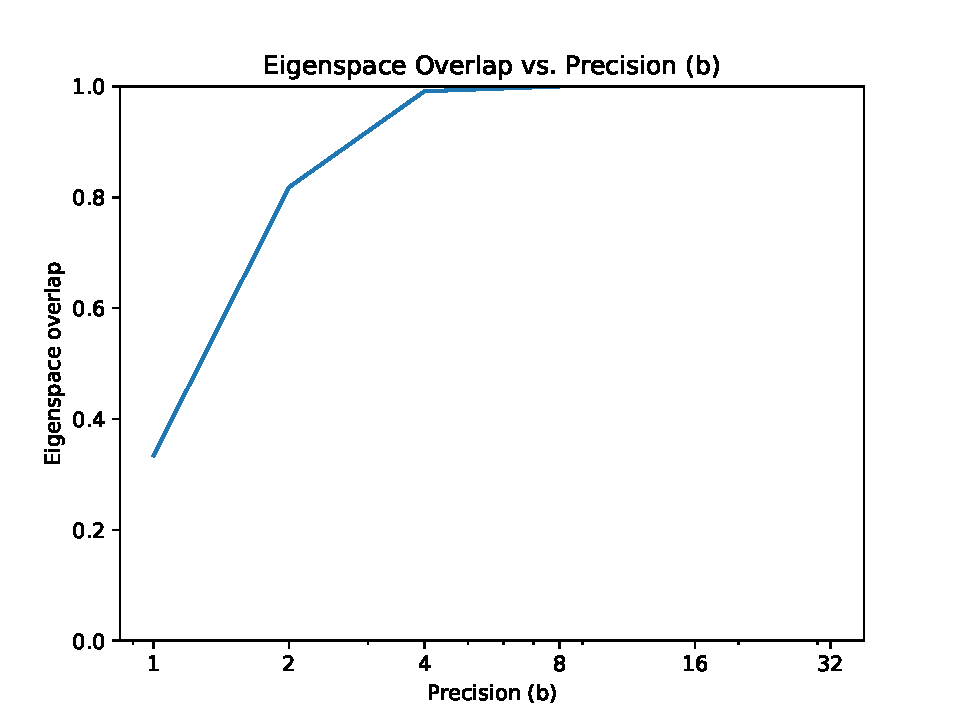
\includegraphics[width=\linewidth]{figures/micro_eig_overlap_vs_precision.pdf} 
\end{tabular}
\caption{Empirical Validation of Theorem~\ref{thm1}. We measure the eigenspace overlap of uniformly quantized embeddings with the uncompressed embedding for various precisions ($b\in\{1,2,4,8,16,32\}$), and observe the eigenspace overlap grows quickly as the precision grows.  For the uncompressed embedding, we generate a random matrix $X \in \RR^{10^5 \times 300}$, with each entry drawn uniformly at random in $[-\frac{1}{\sqrt{300}}, \frac{1}{\sqrt{300}}]$.}
\label{fig:micro_eigoverlap_vs_prec}
\end{figure}

%\subsection{Theory validation}
%	\begin{itemize}
%		\item Impact of quantization on overlap 
%			\begin{itemize}
% 				\item Exp 1: overlap vs precision for different dimensionality. Expectation: overlap increases with higher precision.
%				\item Exp2: overlap vs dimensionality for different precision. Expectation: overlap increases with dimensionality. This explains that under fix memory budget, using lower bits quantization can be beneficial
%			\end{itemize}
%		\item The impact of clipping on eigen-subspace overlap
%			\begin{itemize}
%				\item Simulation based experiments on subspace overlap as a function of different clipping threshold and precision. 
%				\item The way we introduce this in: in our main theorem, we assume the dynamic range is $O(1/\sqrt{d})$ as a consequence of the automatic clipping. We want to show here this is the case in practice and then discuss the specific way clipping influence eigenspace overlap.
%			\end{itemize}
%		\item Loop-back discussion on the large scale empirical experiments in Section~\ref{subsec:hard_explain}
%	\end{itemize}

%
%\section{Experiments}
%\label{sec:experiments}
%We now evaluate the performance of our word embedding compression algorithm on a variety of NLP tasks and embeddings types.
We show that our compression method is consistently able to match the performance of more complex baselines (DCCL, k-means), while dramatically outperforming more naive baselines (dimensionality reduction).
We additionally present results in which we maintain the memory budget fixed by  jointly varying the dimension and precision of the compressed embeddings;
we observe that in this memory-constrained setting, the best compressed embeddings attain \todo{XX\%} to \todo{YY\%} better performance than the full-precision embeddings.
This demonstrates the importance of considering low-precision when trying to attain the best possible performance under a memory budget.

\subsection{Large-scale evaluation}
\begin{itemize}
	\item \textbf{Embeddings}: GloVe ($d\in\{50,100,200,300\}$, $n=400k$) and fastText ($d=300$, $n=10^6$) pre-trained.
	\item \textbf{Baselines}: k-means, DCCL, dim. reduction (GloVe)
	\item \textbf{Tasks}: DrQA, sentiment, intrinsics, synthetics.
	\item \textbf{Compression ratios}: 8x-32x.
	\item \textbf{Number of random seeds}: 5
\end{itemize}

In Figure~\ref{fig:drqa_sent_results} we show that on both question answering and sentiment analysis tasks the uniform quantization method performs comparably to k-means and DCCL, while performing significantly better than the dimensionality reduction baseline.

%\begin{figure}
%\begin{center}
%\centerline{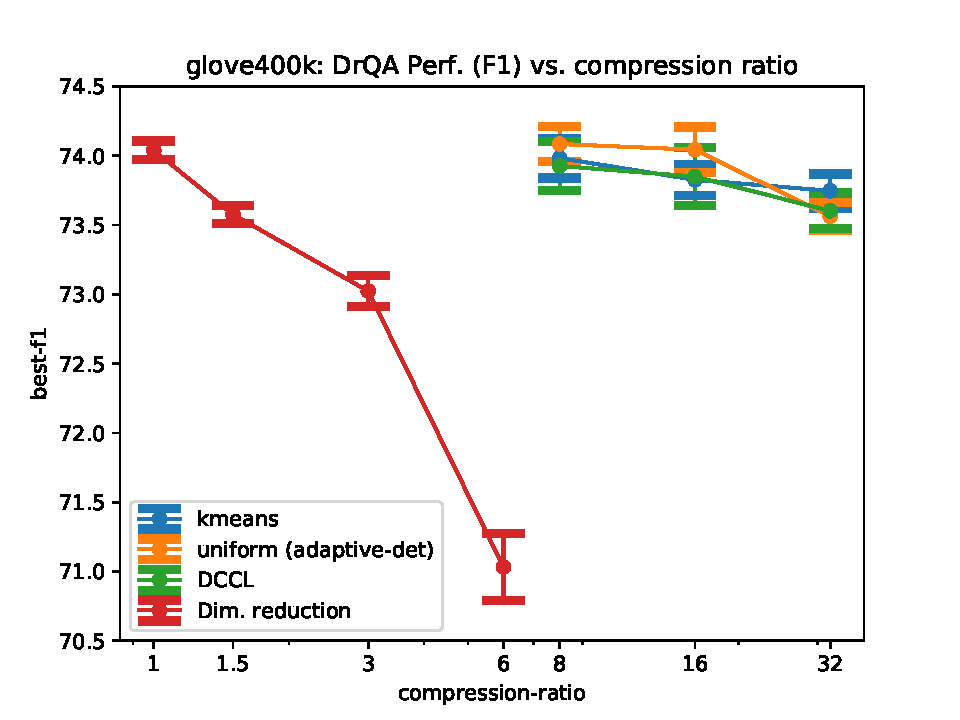
\includegraphics[width=\columnwidth]{figures/glove400k_drqa_vs_compression.pdf}}
%\caption{Question answering performance (DrQA) for a number of compression methods at various compression ratios, on pre-trained GloVe embedding.  Uniform quantization performs similarly to k-means and DCCL, while significantly outperforming the dimensionality reduction baseline. \todo{TODO: Include fastText results (though there won't be a dim. reduction baseline, since they don't release pre-trained embeddings at smaller dimensions.)}}
%\label{fig:glove400k_drqa}
%\end{center}
%\end{figure}

\begin{figure*}
	\centering
	\begin{small}
		%		\begin{tabular}{c c c c}
		\begin{tabular}{@{\hskip -0.0in}c@{\hskip -0.0in}c@{\hskip -0.0in}}
			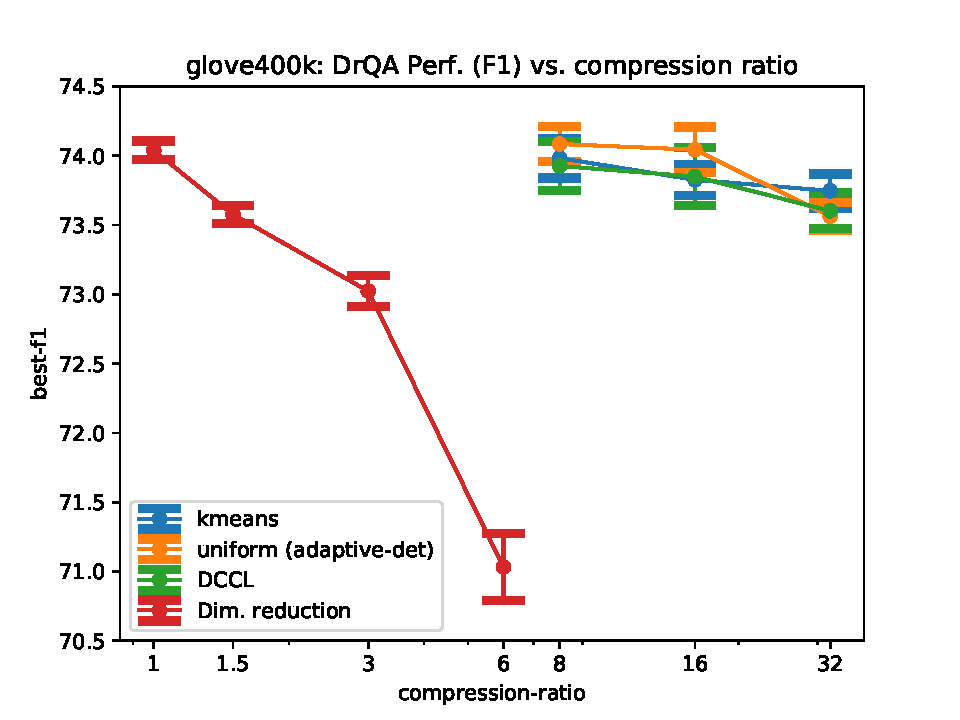
\includegraphics[width=0.4\linewidth]{figures/glove400k_drqa_vs_compression.pdf} &
			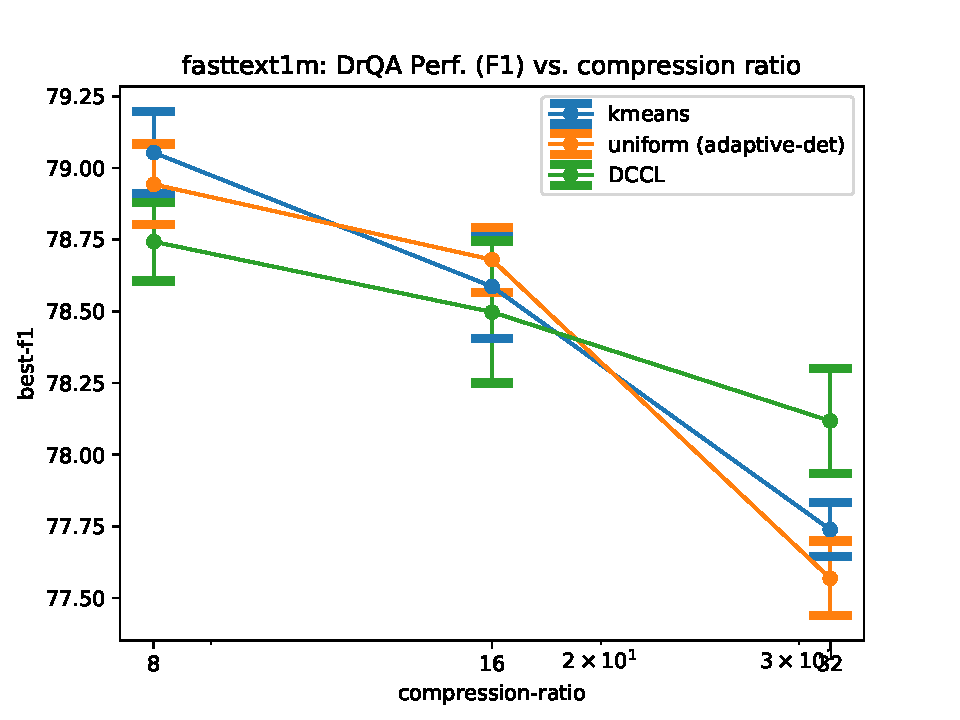
\includegraphics[width=0.4\linewidth]{figures/fasttext1m_drqa_vs_compression.pdf} \\
			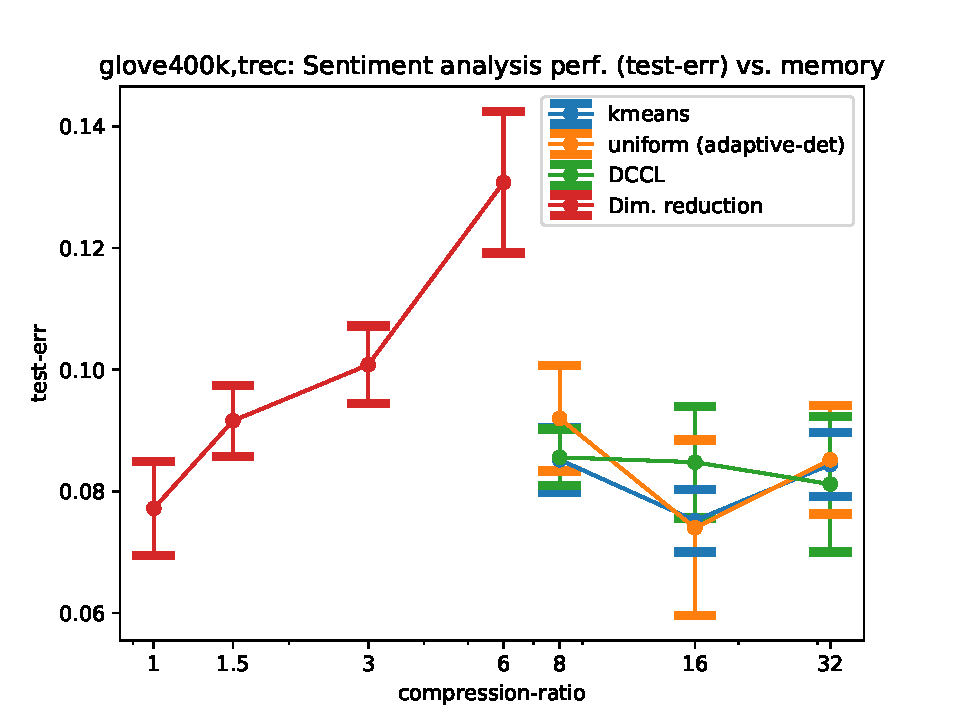
\includegraphics[width=0.4\linewidth]{figures/glove400k_trec_test-err_vs_compression.pdf} &
			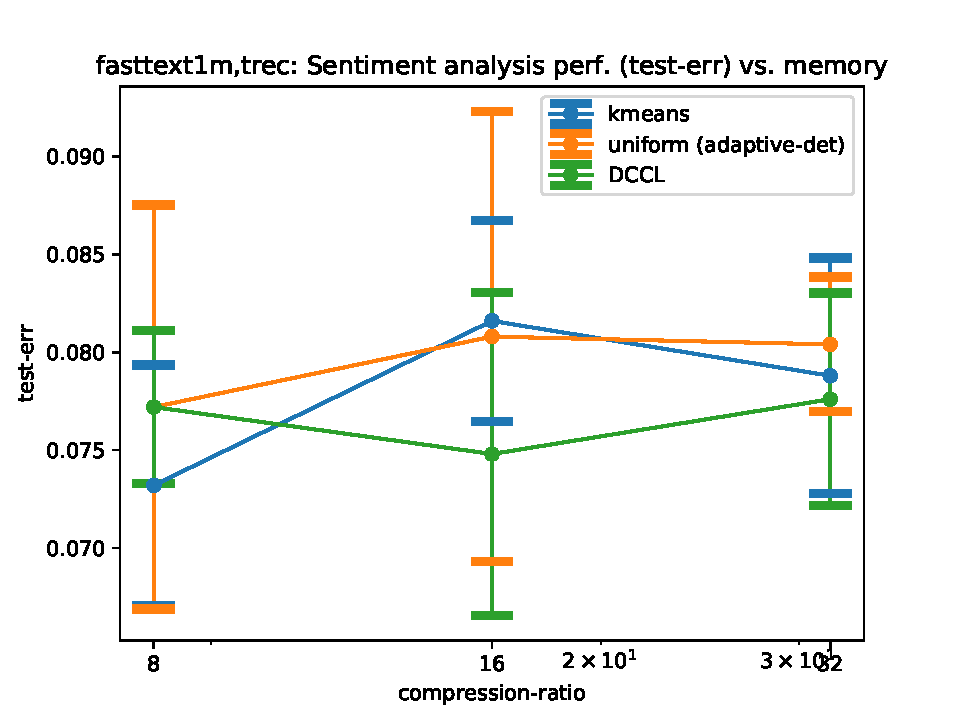
\includegraphics[width=0.4\linewidth]{figures/fasttext1m_trec_test-err_vs_compression.pdf} \\
			\;\;\;\;\;(a) & \;\;\;\;\;\;(b) 
		\end{tabular}
	\end{small}
\caption{Question answering (top) and sentiment analysis (bottom) performance for a number of compression methods at various compression ratios, on pre-trained 300-dimensional GloVe and fastText embeddings.
Uniform quantization performs similarly to k-means and DCCL.  For GloVe, we are also able to compare with pre-trained embeddings of smaller dimensions ($d\in\{50,100,200,300\}$), and observe that compressing the 300-dimensional embeddings is significantly better than using a lower dimension.}
\label{fig:drqa_sent_results}
\end{figure*}

\begin{figure*}
	\centering
	\begin{small}
		%		\begin{tabular}{c c c c}
		\begin{tabular}{@{\hskip -0.0in}c@{\hskip -0.0in}c@{\hskip -0.0in}}
			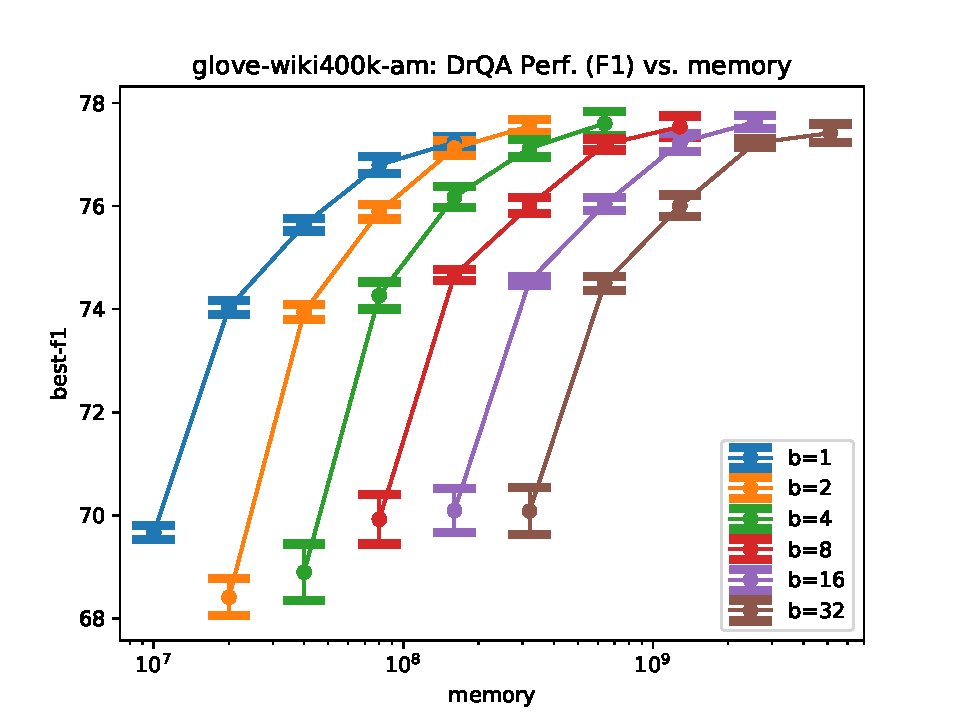
\includegraphics[width=0.4\linewidth]{figures/glove-wiki400k-am_drqa_vs_compression.pdf} &
			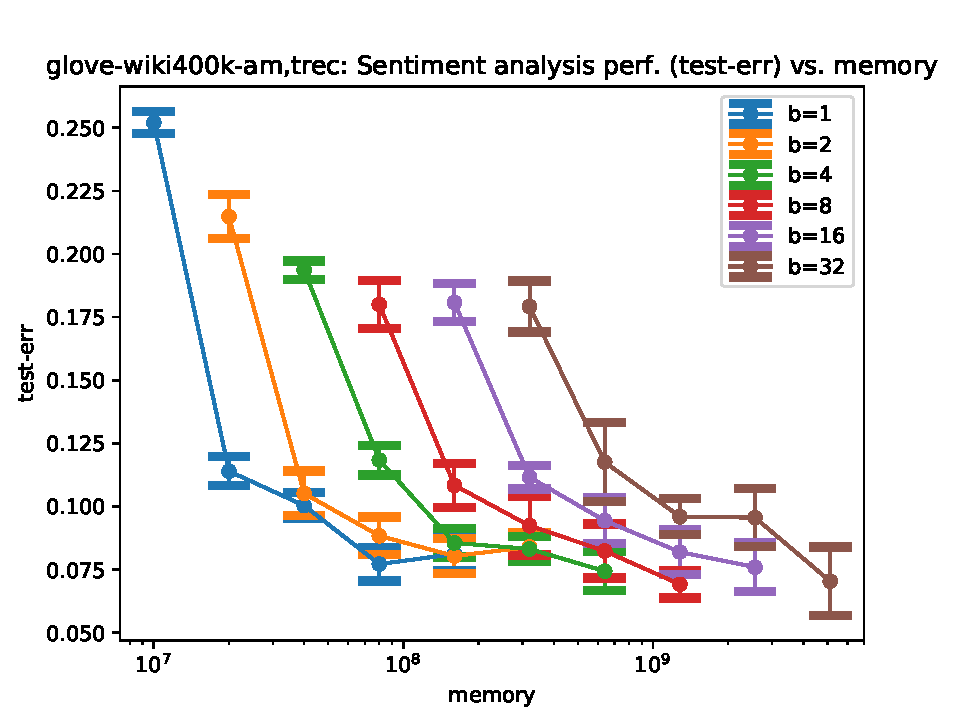
\includegraphics[width=0.4\linewidth]{figures/glove-wiki400k-am_trec_test-err_vs_compression.pdf} \\
			\;\;\;\;\;(a) & \;\;\;\;\;\;(b) 
		\end{tabular}
	\end{small}
	\caption{DrQA and sentiment analysis results (TREC dataset), where we train GloVe embeddings of various dimensions ($d\in\{25,50,100,200,400\}$) and compress them at various precisions ($b \in \{1,2,4,8,16,32\}$) with uniform quantization.  Here we see that when considering a memory budget, it is best to use low-precision features with high-dimensional embeddings.}
	\label{fig:drqa_sent_dimVsPrec}
\end{figure*}

%\begin{figure*}
%	\centering
%	\begin{small}
%		%		\begin{tabular}{c c c c}
%		\begin{tabular}{@{\hskip -0.0in}c@{\hskip -0.0in}c@{\hskip -0.0in}}
%			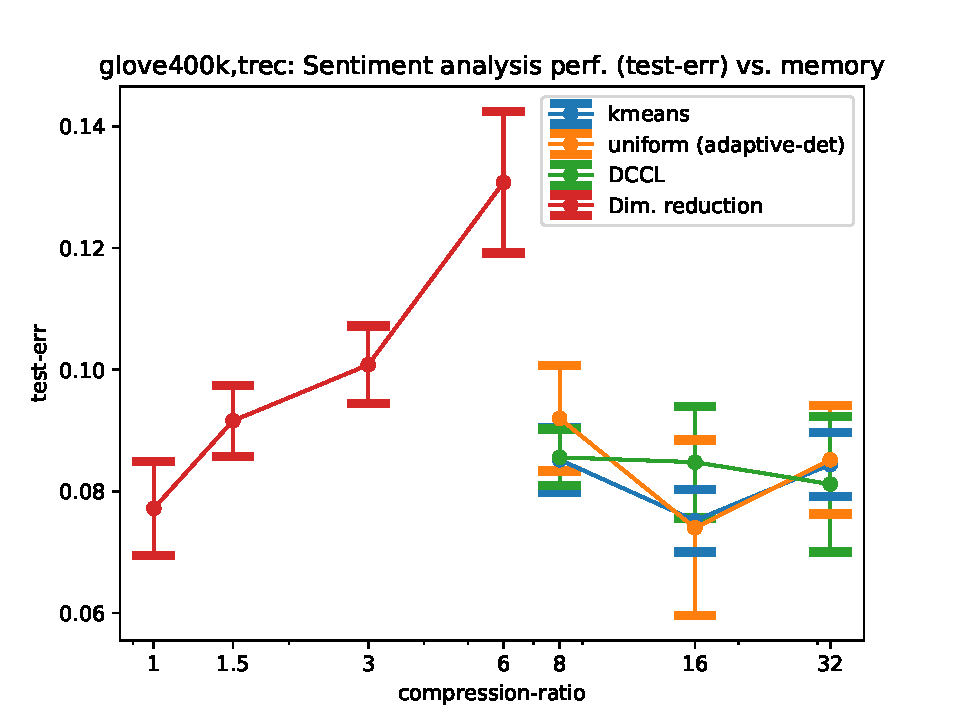
\includegraphics[width=0.45\linewidth]{figures/glove400k_trec_test-err_vs_compression.pdf} &
%			\includegraphics[width=0.45\linewidth]{figures/fasttext1m_trec_test-err_vs_compression.pdf} \\
%			\;\;\;\;\;(a) & \;\;\;\;\;\;(b) 
%		\end{tabular}
%	\end{small}
%	\caption{Sentiment analysis results (TREC dataset).}
%	\label{fig:sentiment}
%\end{figure*}

\subsection{Fixed budget experiments}
\begin{itemize}
	\item \textbf{Embeddings}: We train GloVe embeddings on a Wiki 2017 dump, for $n=400k$ and $d \in \{25,50,100,200,400,800\}$.
	\item \textbf{Bitrates}: We compress embeddings for $b \in \{1,2,4,8,16,32\}$.
	\item \textbf{Tasks}: DrQA, sentiment, intrinsics, synthetics.
	\item \textbf{Number of random seeds}: 5
\end{itemize}

In Figure~\ref{fig:drqa_sent_dimVsPrec}, we show that when considering a fixed memory budget, it is best to use low-precision and high-dimensions, on both question answering and sentiment analysis tasks.

%\begin{figure}
%	\begin{center}
%		\centerline{\includegraphics[width=\columnwidth]{figures/glove-wiki400k-am_drqa_vs_compression.pdf}}
%		\caption{We compress GloVe embeddings for dimensions $d\in\{25,50,100,200,400\}$ at precision values $b\in\{1,2,4,8,16,32\}$, and measure performance on question-answering (DrQA).  \todo{TODO: Include $d=800$ results, which are worse than $d=400$?}}
%		\label{fig:glove400k_dim_vs_prec}
%	\end{center}
%\end{figure}

%
%\section{Theory}
%\label{sec:theory}
%%In this section, we analyze the impact of uniform quantization on the generalization performance of linear regression models trained on top of the word embeddings.
We present two results:
First, we show that when the embedding matrix is quantized to $b$ bits, and the linear ridge regression model is trained with regularization parameter $\lambda$, we attain good generalization bounds for the quantized features relative to the full-precision features when $2^b \lambda$ is large.
Second, we show that if the singular values of the embedding matrix decay slowly, then training the regression model with a large regularization parameter $\lambda$ cannot perform much worse than training with a smaller one.
Combining this theoretical result with our empirical observation that the singular values of embedding matrices typically decay slowly provides a principled explanation for why low-precision embeddings perform well on various tasks.

We begin, however, by reviewing generalization bounds for fixed design linear ridge regression.

\subsection{Background: Generalized Bounds for Fixed Design Linear Ridge Regression}
In fixed design linear regression, one is given a dataset $\{(x_i,y_i)\}_{i=1}^n$, for $x_i \in \RR^d$ and $y_i = \by_i + \eps_i \in \RR$, where the $\eps_i$ are independent random perturbations of the ``true labels'' $\by_i$ satisfying $\expect{}{\eps_i} = 0$ and $\var{}{\eps_i} = \sigma^2 < \infty$.
The goal is to design a training algorithm which takes as input the noisy dataset $\{(x_i,y_i)\}_{i=1}^n$ and outputs a model $f(x) = w^T x$ for which $\expect{}{\frac{1}{n}\sum_i (f(x_i) -\by_i)^2} \eqdef \cR(f)$ is small.
Linear ridge regression selects $w^* = \argmin_w \sum_i (w^T x_i - y_i)^2 + \lambda\|w\|_2^2$.
Letting $X \in \RR^{n\times d}$ be the matrix whose rows are $x_i$, $y \defeq (y_1,...,y_n) \in \RR^d$, and $I_d$ be the $d$-dimensional identity matrix, the minimizer of this optimization problem is $w^* = ( X^T X + \lambda I_d)^{-1}X^Ty$.
It is easy to show \citep{alaoui15} that the expected generalization error for the model $f_X(x) \defeq w^{*T}x$ is
\begin{eqnarray*}
\cR(f_X) &=& \frac{\lambda^2}{n} \by^T(XX^T + \lambda I_n)^{-2}\by \; +\\ && \frac{\sigma^2}{n}\tr\Big((XX^T)^2(XX^T + \lambda I_n)^{-2}\Big).
\end{eqnarray*}

The question we ask in this work is: when we replace $X$ by an approximation $\tX$, how close will $\cR(f_{\tX})$ be to $\cR(f_X)$?
To answer this question, we intuitively require two things: a notion of distance between $X$ and $\tX$, and an upper bound for $\cR(f_{\tX})$ in terms of $\cR(f_X)$ and the distance between $X$ and $\tX$.
For both of these components, we leverage the recent work of \citep{lprff18}.
In that work, they define the following notion of distance between two matrices:

\begin{definition}{\citep{lprff18}}
	\label{def:specdist}
	For $\Delta_1, \Delta_2 \geq 0$, a symmetric matrix $A$ is a \emph{$(\Delta_1, \Delta_2)$-spectral approximation} of another symmetric matrix $B$ if $(1-\Delta_1)B \preceq A \preceq (1+\Delta_2)B$. 
\end{definition}

By applying this definition to $\tX\tX^T + \lambda I_n$ and $XX^T + \lambda I_n$, the authors prove the following generalization bound:
\begin{proposition}{(Adapted from \citep{lprff18})}
	Let $K \defeq XX^T$ and $\tK \defeq \tX\tX^T$, and suppose $\tK + \lambda I_n$ is $(\Delta_1, \Delta_2)$-spectral approximation of $K+\lambda I_n$, for $\Delta_1 \in [0,1)$, $\Delta_2 \geq 0$.
	Let $d$ denote the rank of $\tX$, and let $f_{X}$ and $f_{\tX}$ be the ridge regression estimators learned using these matrices, with regularizing constant $\lambda \geq 0$ and label noise variance $\sigma^2 < \infty$. Then
	\begin{equation}
	\cR(f_{\tX}) \leq \frac{1}{1-\Delta_1} \hcR(f_X) +  \frac{\Delta_2}{1+\Delta_2}\frac{d}{n}\sigma^2,
	\label{eq:risk_bound}
	\end{equation}
	where 
	\begin{eqnarray*}
	\hcR(f_X) &\defeq& \frac{\lambda}{n} \by^T(K+\lambda I)^{-1}\by + \frac{\sigma^2}{n}\tr\Big(K(K+\lambda I)^{-1}\Big) \\
	&\geq& \cR(f_X).
%	\label{eq:avron_rhat}
	\end{eqnarray*}
	\label{prop:genbound}
\end{proposition}
\todo{Discuss how what we will show differs from what is shown in kernel paper.}

\subsection{Theoretical Results}
We now show that our compression algorithm with high probability produces an embedding matrix which is a close spectral approximation of the full-precision matrix, in terms of $(\Delta_1,\Delta_2)$.
Combining this with the Proposition~\ref{prop:genbound} yields a generalization bound for the compressed embeddings.
A consequence of our bound is that when the regularization parameter is large, lower precision can be used for the embeddings without affecting $\Delta_1$ and $\Delta_2$.
We show that in the case of word embeddings with slowly-decaying singular values, a large regularization parameter $\lambda$ (and thus, a low-precision $b$) can be used without significantly affecting generalization performance.
Our empirical observation that embedding matrices have slowly decaying singular values thus helps explain why our compression algorithm is able to attain strong generalization performance at very low levels of precision.

We now present our main theoretical result, deferring all proofs to the Appendix:
\begin{theorem}
	\label{thm:main}
	Let $X \in \RR^{n\times d}$ be an embedding matrix with corresponding Gram matrix $K \defeq XX^T$, where we assume all entries $X_{ij} \in [-\frac{1}{\sqrt{d}},\frac{1}{\sqrt{d}}]$; let $\tX\defeq X+C$ denote a $b$-bit quantization of $X$, with $\tK \defeq \tX\tX^T$ the kernel matrix of the quantized data matrix. Here, $C$ denotes the quantization noise, with $\expect{}{C_{ij}} = 0$ and $\var{}{C_{ij}} \leq \delta_b^2/d \;\;\forall i,j$, where $\delta_b^2 \defeq (2^b-1)^{-2}$, and $b$ is the number of bits used per feature.
	Then for any $\Delta_1 \geq 0, \Delta_2 \geq \delta^2_b/\lambda$,
	\begin{eqnarray*}
	&&\hspace{-0.37in}\Prob\Big[(1- \Delta_1) (K + \lambda I_n) \preceq \tK + \lambda I_n \preceq (1 + \Delta_2) (K + \lambda I_n)
	\Big] 
	\\ &\geq& 1 - 
	n \exp \bigg(\frac{-\Delta_1^2}{2dL^2 + (2L/3)\Delta_1}\bigg) \\
	&&- n \exp \bigg(\frac{-(\Delta_2-\delta_b^2/\lambda)^2}{2dL^2 + (2L/3)(\Delta_2-\delta_b^2/\lambda)}\bigg),
	\end{eqnarray*}
	for $L \defeq 5 \cdot \frac{2^b \cdot \delta_b^2}{\lambda}\cdot \frac{n}{d}$.
\end{theorem}
\todo{Discuss assumption of bounded embedding entries.}\\
Note that in this theorem, we assume the embedding matrix is bounded, whereas in the actual implementation of our compression algorithm (Alg.~\ref{alg:smallfry}) we enforce this constraint artificially by searching for the optimal threshold at which to clip the matrix entries.
To better understand the implications of the above theorem, we present the following corollary:
\begin{corollary}
	\label{cor:main}
	If $\Delta_1 \geq \frac{\log(n/\rho)L}{3}\Big(1+\sqrt{1+\frac{18d}{\log(n/\rho)}}\Big) \approx \frac{5n}{2^b \lambda}\sqrt{\frac{2\log(n/\rho)}{d}}$,
	then $\Prob\big[(1 - \Delta_1) (K + \lambda I_n) \preceq \tK + \lambda I_n \big] \geq  1 - \rho$. 
	Similarly, if $\Delta_2 \geq \frac{\delta_b^2}{\lambda} +  \frac{\log(n/\rho)L}{3}\Big(1+\sqrt{1+\frac{18d}{\log(n/\rho)}}\Big) \approx \frac{1}{2^{2b}\lambda} + \frac{5n}{2^b \lambda}\sqrt{\frac{2\log(n/\rho)}{d}}$,
	then $\Prob\big[\tK + \lambda I_n \preceq (1 + \Delta_2) (K + \lambda I_n)\big] \geq  1 - \rho$. 
\end{corollary}

This corollary makes clear that if $2^b\lambda$ is large, the $b$-bit compressed embedding matrix will be a close spectral approximation of the full-precision matrix, for small $\Delta_1$ and $\Delta_2$.
In the following theorem, we show that when the smallest singular value of $X^TX$ is large, using a large regularization parameter $\lambda$ will not significantly harm the generalization performance of $f_X$, relative to using a smaller $\lambda$.
Combining this result with Proposition~\ref{prop:genbound} and Theorem~\ref{thm:main}, we can conclude that the generalization performance of a linear model trained on low-precision features with a large regularizer $\lambda$ will not be much worse than the performance of a model trained on the full-precision features with any $\lambda' \leq \lambda$.
We now present the result:

\begin{theorem}
	\label{thm:large_lambda}
	Let $X$ be an embedding matrix, and $\by$ be the corresponding vector of labels. Let $\sm$ be the smallest eigenvalue of $X^T X$, and let $\lambda_1, \lambda_2$ be two scalars such that $0 \leq \lambda_1 \leq \lambda_2 \leq a\cdot \sm$, for some $a \in [0,1]$. Letting $\cR_{\lambda}(K)$ denote the expected loss when training with regularizer $\lambda$, Gram matrix $K = XX^T$, and label noise $\sigma^2$, we get that:
	\begin{equation}
	R_{\lambda_2}(XX^T) - R_{\lambda_1}(XX^T) \leq a^2\|y\|^2/n
	\label{eq1}
	\end{equation}
\end{theorem}
Intuitively, this theorem shows that if there are no directions in the input space with very small variance, then using a large regularizer will not hurt performance significantly relative to using a smaller regularizer.
This makes sense because the directions of small variance are the ones which are effectively ignored when strong regularization is used.
For the purposes of this work, this theorem shows that if the embedding matrix has a large smallest eigenvalue, it should be possible to attain strong generalization performance with low-precision and a large regularizer.
In practice, we observe that it is common for embedding matrices to have slowly decaying spectra, and thus have a large smallest eigenvalue;
we present plots of the singular values for fastText and Glove embeddings in Figure~\ref{fig:real_spectra}.

\subsection{Empirical Validation of Theory}
In this section, we empirically validate two important predictions made by the above theoretical results:
\begin{enumerate}
	\item When $2^b \lambda$ is large, $\Delta_1$ and $\Delta_2$ are small (Figure~\ref{fig:micro_d1d2}).
	\item When $X^T X$ has a large smallest eigenvalue, generalization performance is not significantly harmed by using a large regularizer
	(Figure~\ref{fig:micro_large_sigma_min}).
\end{enumerate}

In addition, we show that in general word embedding matrices have a relatively large smallest singular value (Figure~\ref{fig:real_spectra}).

\begin{figure*}
	\centering
	\begin{tabular}{c c}
		%		\begin{tabular}{@{\hskip -0.0in}c@{\hskip -0.0in}c@{\hskip -0.0in}c@{\hskip -0.0in}}
		\includegraphics[width=0.4\linewidth]{figures/micro_uniform_nonadapt_delta1_vs_2_b_lambda.pdf} &	
		\includegraphics[width=0.4\linewidth]{figures/micro_uniform_nonadapt_delta2_vs_2_b_lambda.pdf}
	\end{tabular}
	\caption{We plot $\Delta_1$ (left) and $\Delta_2$ (right) as a function of $2^b\lambda$, on a randomly generated matrix $X\in\RR^{1000\times 30}$ ($X_{ij}\sim U([-\frac{1}{\sqrt{30}},\frac{1}{\sqrt{30}}])$), for various precisions $b$ and $\lambda$ values.  We show that $2^b \lambda$ largely determines the values of $\Delta_1$ and $\Delta_2$ after compression, as predicted by our theoretical results. We plot results for both deterministic quantization and stochastic quantization, and see that they perform quite similarly by these metrics (though deterministic does perform slightly better on $\Delta_2$). We additionally plot the bounds for $\Delta_1$ and $\Delta_2$ from Corollary~\ref{cor:main}, and see that while the bounds are not tight, their trajectory is matched by the real data.}
	\label{fig:micro_d1d2}
\end{figure*}

\begin{figure}
	\begin{center}
		\centerline{\includegraphics[width=0.8\columnwidth]{figures/micro_large_sigma_min.pdf}}
		\caption{We show that the ratio $a=\frac{\lambda}{\sigma_{min}}$ between the regularization parameter $\lambda$ and the smallest eigenvalue $\sigma_{min}$ of $X^T X$ is very predictive of the degradation in generalization performance $\|\by - y_{pred}\|^2/\|\by\|^2$, as predicted by Theorem~\ref{thm:large_lambda}.
		In particular, we generate an i.i.d. Gaussian matrix $X\in \RR^{1000\times 2}$ for various standard deviations $\sigma$, and consider the noiseless model $\by_i = [0,1]^T x_i$.
		We then solve for the optimal ridge regression model for various values of $\lambda$, and plot $a$ vs.\ the normalized degradation in generalization performance of this model. \todo{TODO: Perhaps plot a more realistic example?}
		}
		\label{fig:micro_large_sigma_min}
	\end{center}
\end{figure}

\begin{figure*}
	\centering
	\begin{tabular}{c c}
		%		\begin{tabular}{@{\hskip -0.0in}c@{\hskip -0.0in}c@{\hskip -0.0in}c@{\hskip -0.0in}}
		\includegraphics[width=0.4\linewidth]{figures/glove400k_spectra.pdf} &	
		\includegraphics[width=0.4\linewidth]{figures/fasttext1m_spectra.pdf}
	\end{tabular}
	\caption{We plot the real spectra of the pre-trained GloVe ($d \in \{50,100,200,300\}$) and fastText ($d=300$) embedding matrices.
	The smallest singular values are generally only 1 or 2 orders of magnitude smaller than the largest.}
	\label{fig:real_spectra}
\end{figure*}

\subsection{Effect of Clipping on $(\Delta_1,\Delta_2)$}
One way to understand why it is important for us to search for the optimal clipping value in Algorithm~\ref{alg:smallfry} is by understanding the way clipping and quantization together impact $\Delta_1$ and $\Delta_2$.
This perspective reveals that there is a fundamental trade-off between $\Delta_1$ and $\Delta_2$ when choosing the clipping value:
if the clip value is too large, then $\Delta_2$ becomes very large, while if the clip value is too small, then $\Delta_1$ becomes very large.
We demonstrate this in Figure~\ref{fig:deltas_vs_clip_quant}
\begin{figure}
	\begin{center}
		\centerline{\includegraphics[width=0.8\columnwidth]{figures/deltas_vs_clip_and_quant.pdf}}
		\caption{On random Gaussian data $X \in \RR^{1000\times 30}$, we demonstrate the joint effect of clipping and quantizing on $\Delta_1$ and $\Delta_2$, where we take $\lambda = \sigma_{min}(X^T X)/10$.
		A large clipping value gives large $\Delta_2$, whereas a small clipping values gives large $\Delta_1$.
		This reveals the importance of choosing a clipping value which balances these two considerations.
		}
		\label{fig:deltas_vs_clip_quant}
	\end{center}
\end{figure}


%\section{Jian Version Theory Parts}
In this section, we work on theoretically understand why uniformly quantized embeddings can perform similarly to uncompressed embeddings on downstream tasks.  
Our analysis reveals that when the uncompressed embedding has a slow-decaying spectrum (which we empirically observe to be true), uniform quantization can have negligible effect on the generalization bound for downstream models on top of the embedding. As a consequence, the quantized embeddings can perform similarly as the uncompressed one. 
Specifically, we analyze the impact of quantization on generalization bound in the case of linear ridge regression, which is the simplification and basis of many classification and regression models in NLP\footnote{Classification tasks can cast as regression over probabilities.}. We begin with the background on generalization bound for fixed design linear ridge regression in Section~\ref{subsec:fixed_design}, and then discuss our theoretically analysis based on this generalization bound in details in Section~\ref{subsec:theo_core}. We validate our theory with experiments in Section~\ref{subsec:emp_valid}. \todo{how to add section 6.4}

%In this section, we work on theoretically understand why uni- formly quantized embeddings can perform similarly to un- compressed embeddings on downstream tasks. Our analysis reveals that uniform ly quantized em beddings can perform sim ilarly as a consequence of com bining two factors: 1) quantization can have negligible effect on generalization if the standard deviation of quantization noise is small relative to regularization strength; 2) when embedding matrices has slow-decaying spectra (which we empirically observe to be true), large regularizer has minimal inuence on generaliza- tion. Specically, we analyze the impact of quantization on generalization bound in the case of linear ridge regression, which is the simplication and basis of many classication and regression m odels in N L P 2 . We begin w ith the back- ground on generalization bound for xed design linear ridge regression in Section 6.1. We then discuss our theoretically analysis based on this generalization bound in details in Section 6.2

\subsection{Background: Generalized Bounds for Fixed Design Linear Ridge Regression}
\label{subsec:fixed_design}
In fixed design linear ridge regression, one is given a dataset $\{(x_i,y_i)\}_{i=1}^n$, for $x_i \in \RR^d$ and $y_i = \by_i + \eps_i \in \RR$, where the $\eps_i$ are independent random perturbations of the ``true labels'' $\by_i$ satisfying $\expect{}{\eps_i} = 0$ and $\var{}{\eps_i} = \sigma^2 < \infty$.
The goal is to design a training algorithm which takes as input the noisy dataset $\{(x_i,y_i)\}_{i=1}^n$ and outputs a model $f(x) = w^T x$ for which $\expect{}{\frac{1}{n}\sum_i (f(x_i) -\by_i)^2} \eqdef \cR(f)$ is small.
As a empirical risk minimization problem, linear ridge regression selects $w^* = \argmin_w \sum_i (w^T x_i - y_i)^2 + \lambda\|w\|_2^2$ with regularizer strength $\lambda$.
Letting $X \in \RR^{n\times d}$ be the matrix whose rows are $x_i$, $y \defeq (y_1,...,y_n) \in \RR^d$, and $I_d$ be the $d$-dimensional identity matrix, the minimizer of this optimization problem is $w^* = ( X^T X + \lambda I_d)^{-1}X^Ty$.
It is easy to show \citep{alaoui15} that the expected generalization error for the model $f_X(x) \defeq w^{*T}x$ is
\begin{eqnarray*}
\cR(f_X) &=& \frac{\lambda^2}{n} \by^T(XX^T + \lambda I_n)^{-2}\by \; +\\ && \frac{\sigma^2}{n}\tr\Big((XX^T)^2(XX^T + \lambda I_n)^{-2}\Big).
\end{eqnarray*}

The question we ask in this work is: when we replace uncompressed embedding $X$ by an approximation $\tX$, how close will $\cR(f_{\tX})$ be to $\cR(f_X)$?
To answer this question, we intuitively require two things: a notion of distance between $X$ and $\tX$, and an upper bound for $\cR(f_{\tX})$ in terms of $\cR(f_X)$ and the distance between $X$ and $\tX$.
For both of these components, we build on the recent work of \citep{lprff18}.
In this work, we leverage the following notion of distance between the two matrices $X$ and $\tX$:

\begin{definition}{\citep{lprff18}}
	\label{def:specdist}
	For $\Delta_1, \Delta_2 \geq 0$, a symmetric matrix $A$ is a \emph{$(\Delta_1, \Delta_2)$-spectral approximation} of another symmetric matrix $B$ if $(1-\Delta_1)B \preceq A \preceq (1+\Delta_2)B$. 
\end{definition}

Substituting with $A=\tX\tX^T + \lambda I_n$ and $B=XX^T + \lambda I_n$, we can derive the generalization bound for fixed design linear regression on top of approximation $\tX$ in Proposition~\ref{prop:genbound}.
\begin{proposition}{(Adapted from \citep{lprff18})}
	Let $K \defeq XX^T$ and $\tK \defeq \tX\tX^T$, and suppose $\tK + \lambda I_n$ is $(\Delta_1, \Delta_2)$-spectral approximation of $K+\lambda I_n$, for $\Delta_1 \in [0,1)$, $\Delta_2 \geq 0$.
	Let $d$ denote the rank of $\tX$, and let $f_{X}$ and $f_{\tX}$ be the ridge regression estimators learned using these matrices, with regularizing constant $\lambda \geq 0$ and label noise variance $\sigma^2 < \infty$. Then
	\begin{equation}
	\cR(f_{\tX}) \leq \frac{1}{1-\Delta_1} \hcR(f_X) +  \frac{\Delta_2}{1+\Delta_2}\frac{d}{n}\sigma^2,
	\label{eq:risk_bound}
	\end{equation}
	where 
	\begin{eqnarray*}
	\hcR(f_X) &\defeq& \frac{\lambda}{n} \by^T(K+\lambda I)^{-1}\by + \frac{\sigma^2}{n}\tr\Big(K(K+\lambda I)^{-1}\Big) \\
	&\geq& \cR(f_X).
	\label{eq:avron_rhat}
	\end{eqnarray*}
	\label{prop:genbound}
\end{proposition}
\todo{Discuss how what we will show differs from what is shown in kernel paper. Is this necessary?}

Based this generalization bound in~\eqref{eq:avron_rhat} and the notion of $(\Delta_1, \Delta_2)$-spectral approximation in Definition~\ref{def:specdist}, we discuss in details why uniformly quantized embeddings can perform similarly to uncompressed embedding for fixed design linear ridge regression in section~\ref{subsec:theo_core}.

\subsection{Generalization Analysis of Quantized Embeddings}
\label{subsec:theo_core}
Building on Section~\ref{subsec:fixed_design}, we work on to show that when uncompressed embedding $X$ has a slow-decaying spectrum (aligning with our empirical observations), uniform quantization with high probability produces an approximation $\hat{X}$ with small $(\Delta_1, \Delta_2)$; this small $(\Delta_1, \Delta_2)$ then implies that $R(f_{\hat{X}})$, the generalization bound of quantized embedding is close to $R(f_{X})$, the bound for uncompressed embedding $X$. Our proof are achieved in two steps. We first show that when the standard deviation of quantization noise is small relative to regularization strength $\lambda$, a uniformly quantized embedding with high probability achieve close $(\Delta_1, \Delta_2)$-spectral approximation to uncompressed one. Then we show when an uncompressed embedding has slow-decaying spectrum, large regularizer minimally increase the generalization bound comparing to small regularizer. Combining these two steps, we can explain that a uniformly quantized embedding performs similarly to uncompressed one as a consequence of being a close $(\Delta_1, \Delta_2)$-spectral approximation.

%1. We show our theory is on when slow decay, it can minimally affect the generalization.
%2. We first show with high probability, quantized matrix is a close delta 1 delta 2 approximation, inducing low bound, with relatively large regularizer.
%3. We then demonstrate, embedding matrix has empirically slow decaying spectrum, which implies can tolerate large regularizer.
%5. To have a full picture we also discuss on the trade off between A and B on clipping.
%4. We defer all the proof.

%In Thereom we present and use Corollary to discuss the impact of quantization on the generalization bound.

%Theorem 5.

%The reason why we have this is the intuition + empirical validation

%Rewrite col 5.1.

Summarize the message + tell in the next we show, this will together show can have good generalization performance.




%We now show that our compression algorithm with high probability produces an embedding matrix which is a close spectral approximation of the full-precision matrix, in terms of $(\Delta_1,\Delta_2)$.
%Combining this with the Proposition~\ref{prop:genbound} yields a generalization bound for the compressed embeddings.
%A consequence of our bound is that when the regularization parameter is large, lower precision can be used for the embeddings without affecting $\Delta_1$ and $\Delta_2$.
%We show that in the case of word embeddings with slowly-decaying singular values, a large regularization parameter $\lambda$ (and thus, a low-precision $b$) can be used without significantly affecting generalization performance.
%Our empirical observation that embedding matrices have slowly decaying singular values thus helps explain why our compression algorithm is able to attain strong generalization performance at very low levels of precision.

We now present our main theoretical result in Theorem~\ref{thm:main} and use Corollary~\ref{cor:main} to discuss the impact of quantization on  $(\Delta_1, \Delta_2)$. We defer all proofs to the Appendix.
\begin{theorem}
	\label{thm:main}
	Let $X \in \RR^{n\times d}$ be an embedding matrix with corresponding Gram matrix $K \defeq XX^T$, where we assume all entries $X_{ij} \in [-\frac{1}{\sqrt{d}},\frac{1}{\sqrt{d}}]$; let $\tX\defeq X+C$ denote a $b$-bit quantization of $X$, with $\tK \defeq \tX\tX^T$ the kernel matrix of the quantized data matrix. Here, $C$ denotes the quantization noise, with $\expect{}{C_{ij}} = 0$ and $\var{}{C_{ij}} \leq \delta_b^2/d \;\;\forall i,j$, where $\delta_b^2 \defeq (2^b-1)^{-2}$, and $b$ is the number of bits used per feature.
	Then for any $\Delta_1 \geq 0, \Delta_2 \geq \delta^2_b/\lambda$,
	\begin{eqnarray*}
	&&\hspace{-0.37in}\Prob\Big[(1- \Delta_1) (K + \lambda I_n) \preceq \tK + \lambda I_n \preceq (1 + \Delta_2) (K + \lambda I_n)
	\Big] 
	\\ &\geq& 1 - 
	n \exp \bigg(\frac{-\Delta_1^2}{2dL^2 + (2L/3)\Delta_1}\bigg) \\
	&&- n \exp \bigg(\frac{-(\Delta_2-\delta_b^2/\lambda)^2}{2dL^2 + (2L/3)(\Delta_2-\delta_b^2/\lambda)}\bigg),
	\end{eqnarray*}
	for $L \defeq 5 \cdot \frac{2^b \cdot \delta_b^2}{\lambda}\cdot \frac{n}{d}$.
\end{theorem}
\todo{Discuss assumption of bounded embedding entries.}\\
Note that in this theorem, we assume the embedding matrix is bounded, whereas in the actual implementation of our compression algorithm (Alg.~\ref{alg:smallfry}) we enforce this constraint artificially by searching for the optimal threshold at which to clip the matrix entries.
To better understand the implications of the above theorem, we present the following corollary:
\begin{corollary}
	\label{cor:main}
	If $\Delta_1 \geq \frac{\log(n/\rho)L}{3}\Big(1+\sqrt{1+\frac{18d}{\log(n/\rho)}}\Big) \approx \frac{5n \delta_b}{ \lambda}\sqrt{\frac{2\log(n/\rho)}{d}}$,
	then $\Prob\big[(1 - \Delta_1) (K + \lambda I_n) \preceq \tK + \lambda I_n \big] \geq  1 - \rho$. 
	Similarly, if $\Delta_2 \geq \frac{\delta_b^2}{\lambda} +  \frac{\log(n/\rho)L}{3}\Big(1+\sqrt{1+\frac{18d}{\log(n/\rho)}}\Big) \approx \frac{\delta_b}{2^{b}\lambda} + \frac{5n\delta_b}{\lambda}\sqrt{\frac{2\log(n/\rho)}{d}}$,
	then $\Prob\big[\tK + \lambda I_n \preceq (1 + \Delta_2) (K + \lambda I_n)\big] \geq  1 - \rho$. 
\end{corollary}

This corollary makes clear that if the standard deviation of quantization noise is small relative to regularizer, i.e. $\delta_b/\lambda$ is small, the $b$-bit compressed embedding matrix will be a close spectral approximation of the uncompressed matrix, for small $\Delta_1$ and $\Delta_2$.
In the following theorem, we show that when the smallest singular value of $X^TX$ is large, using a large regularization parameter $\lambda$ will not significantly harm the generalization performance of $f_X$, relative to using a smaller $\lambda$.
Combining this result with Proposition~\ref{prop:genbound} and Theorem~\ref{thm:main}, we can conclude that the generalization performance of a linear model trained on a quantized embedding with a large regularizer $\lambda$ will not be much worse than the performance of a model trained on the uncompressed embedding with any $\lambda' \leq \lambda$.
We now present the result:

\begin{theorem}
	\label{thm:large_lambda}
	Let $X$ be an embedding matrix, and $\by$ be the corresponding vector of labels. Let $\sm$ be the smallest eigenvalue of $X^T X$, and let $\lambda_1, \lambda_2$ be two scalars such that $0 \leq \lambda_1 \leq \lambda_2 \leq a\cdot \sm$, for some $a \in [0,1]$. Letting $\cR_{\lambda}(K)$ denote the expected loss when training with regularizer $\lambda$, Gram matrix $K = XX^T$, and label noise $\sigma^2$, we get that:
	\begin{equation}
	R_{\lambda_2}(XX^T) - R_{\lambda_1}(XX^T) \leq a^2\|y\|^2/n
	\label{eq1}
	\end{equation}
\end{theorem}
Intuitively, this theorem shows that if there are no directions in the input space with very small variance, then using a large regularizer will not hurt performance significantly relative to using a smaller regularizer.
This makes sense because the directions of small variance are the ones which are effectively ignored when strong regularization is used.
For the purposes of this work, this theorem shows that if the embedding matrix has a large smallest eigenvalue, it should be possible to attain strong generalization performance with low-precision and a large regularizer.
Indeed, we observe in practice that it is common for embedding matrices to have slowly decaying spectra, and thus have a large smallest eigenvalue;
we present plots of the singular values for fastText and Glove embeddings in Figure~\ref{fig:real_spectra}. \todo{link to fast decay in kernel approximation paper}

\subsection{Empirical Validation of Theory}
\label{subsec:emp_valid}
In this section, we empirically validate two important predictions made by the above theoretical results:
\begin{enumerate}
	\item When $2^b \lambda$ is large, $\Delta_1$ and $\Delta_2$ are small (Figure~\ref{fig:micro_d1d2}).
	\item When $X^T X$ has a large smallest eigenvalue, generalization performance is not significantly harmed by using a large regularizer
	(Figure~\ref{fig:micro_large_sigma_min}).
\end{enumerate}

In addition, we show that in general word embedding matrices have a relatively large smallest singular value (Figure~\ref{fig:real_spectra}).

\begin{figure*}
	\centering
	\begin{tabular}{c c}
		%		\begin{tabular}{@{\hskip -0.0in}c@{\hskip -0.0in}c@{\hskip -0.0in}c@{\hskip -0.0in}}
		\includegraphics[width=0.4\linewidth]{figures/micro_uniform_nonadapt_delta1_vs_2_b_lambda.pdf} &	
		\includegraphics[width=0.4\linewidth]{figures/micro_uniform_nonadapt_delta2_vs_2_b_lambda.pdf}
	\end{tabular}
	\caption{We plot $\Delta_1$ (left) and $\Delta_2$ (right) as a function of $2^b\lambda$, on a randomly generated matrix $X\in\RR^{1000\times 30}$ ($X_{ij}\sim U([-\frac{1}{\sqrt{30}},\frac{1}{\sqrt{30}}])$), for various precisions $b$ and $\lambda$ values.  We show that $2^b \lambda$ largely determines the values of $\Delta_1$ and $\Delta_2$ after compression, as predicted by our theoretical results. We plot results for both deterministic quantization and stochastic quantization, and see that they perform quite similarly by these metrics (though deterministic does perform slightly better on $\Delta_2$). We additionally plot the bounds for $\Delta_1$ and $\Delta_2$ from Corollary~\ref{cor:main}, and see that while the bounds are not tight, their trajectory is matched by the real data.}
	\label{fig:micro_d1d2}
\end{figure*}

\begin{figure}
	\begin{center}
		\centerline{\includegraphics[width=0.8\columnwidth]{figures/micro_large_sigma_min.pdf}}
		\caption{We show that the ratio $a=\frac{\lambda}{\sigma_{\min}}$ between the regularization parameter $\lambda$ and the smallest eigenvalue $\sigma_{\min}$ of $X^T X$ is very predictive of the degradation in generalization performance $\|\by - y_{pred}\|^2/\|\by\|^2$, as predicted by Theorem~\ref{thm:large_lambda}.
		In particular, we generate an i.i.d. Gaussian matrix $X\in \RR^{1000\times 2}$ for various standard deviations $\sigma$, and consider the noiseless model $\by_i = [0,1]^T x_i$.
		We then solve for the optimal ridge regression model for various values of $\lambda$, and plot $a$ vs.\ the normalized degradation in generalization performance of this model. \todo{TODO: Perhaps plot a more realistic example?}
		}
		\label{fig:micro_large_sigma_min}
	\end{center}
\end{figure}

\begin{figure*}
	\centering
	\begin{tabular}{c c}
		%		\begin{tabular}{@{\hskip -0.0in}c@{\hskip -0.0in}c@{\hskip -0.0in}c@{\hskip -0.0in}}
		\includegraphics[width=0.4\linewidth]{figures/glove400k_spectra.pdf} &	
		\includegraphics[width=0.4\linewidth]{figures/fasttext1m_spectra.pdf}
	\end{tabular}
	\caption{We plot the real spectra of the pre-trained GloVe ($d \in \{50,100,200,300\}$) and fastText ($d=300$) embedding matrices.
	The smallest singular values are generally only 1 or 2 orders of magnitude smaller than the largest.}
	\label{fig:real_spectra}
\end{figure*}

\subsection{Effect of Clipping on $(\Delta_1,\Delta_2)$}
One way to understand why it is important for us to search for the optimal clipping value in Algorithm~\ref{alg:smallfry} is by understanding the way clipping and quantization together impact $\Delta_1$ and $\Delta_2$.
This perspective reveals that there is a fundamental trade-off between $\Delta_1$ and $\Delta_2$ when choosing the clipping value:
if the clip value is too large, then $\Delta_2$ becomes very large, while if the clip value is too small, then $\Delta_1$ becomes very large.
We demonstrate this in Figure~\ref{fig:deltas_vs_clip_quant}
\begin{figure}
	\begin{center}
		\centerline{\includegraphics[width=0.8\columnwidth]{figures/deltas_vs_clip_and_quant.pdf}}
		\caption{On random Gaussian data $X \in \RR^{1000\times 30}$, we demonstrate the joint effect of clipping and quantizing on $\Delta_1$ and $\Delta_2$, where we take $\lambda = \sigma_{\min}(X^T X)/10$.
		A large clipping value gives large $\Delta_2$, whereas a small clipping values gives large $\Delta_1$.
		This reveals the importance of choosing a clipping value which balances these two considerations.
		}
		\label{fig:deltas_vs_clip_quant}
	\end{center}
\end{figure}

%%%\section{Jian Version Theory Parts}
In this section, we work on theoretically understand why uniformly quantized embeddings can perform similarly to uncompressed embeddings on downstream tasks.  
Our analysis reveals that when the uncompressed embedding has a slow-decaying spectrum (which we empirically observe to be true), uniform quantization can have negligible effect on the generalization bound for downstream models on top of the embedding. As a consequence, the quantized embeddings can perform similarly as the uncompressed one. 
Specifically, we analyze the impact of quantization on generalization bound in the case of linear ridge regression, which is the simplification and basis of many classification and regression models in NLP\footnote{Classification tasks can cast as regression over probabilities.}. We begin with the background on generalization bound for fixed design linear ridge regression in Section~\ref{subsec:fixed_design}, and then discuss our theoretically analysis based on this generalization bound in details in Section~\ref{subsec:theo_core}. We validate our theory with experiments in Section~\ref{subsec:emp_valid}. \todo{how to add section 6.4}

%In this section, we work on theoretically understand why uni- formly quantized embeddings can perform similarly to un- compressed embeddings on downstream tasks. Our analysis reveals that uniform ly quantized em beddings can perform sim ilarly as a consequence of com bining two factors: 1) quantization can have negligible effect on generalization if the standard deviation of quantization noise is small relative to regularization strength; 2) when embedding matrices has slow-decaying spectra (which we empirically observe to be true), large regularizer has minimal inuence on generaliza- tion. Specically, we analyze the impact of quantization on generalization bound in the case of linear ridge regression, which is the simplication and basis of many classication and regression m odels in N L P 2 . We begin w ith the back- ground on generalization bound for xed design linear ridge regression in Section 6.1. We then discuss our theoretically analysis based on this generalization bound in details in Section 6.2

\subsection{Background: Generalized Bounds for Fixed Design Linear Ridge Regression}
\label{subsec:fixed_design}
In fixed design linear ridge regression, one is given a dataset $\{(x_i,y_i)\}_{i=1}^n$, for $x_i \in \RR^d$ and $y_i = \by_i + \eps_i \in \RR$, where the $\eps_i$ are independent random perturbations of the ``true labels'' $\by_i$ satisfying $\expect{}{\eps_i} = 0$ and $\var{}{\eps_i} = \sigma^2 < \infty$.
The goal is to design a training algorithm which takes as input the noisy dataset $\{(x_i,y_i)\}_{i=1}^n$ and outputs a model $f(x) = w^T x$ for which $\expect{}{\frac{1}{n}\sum_i (f(x_i) -\by_i)^2} \eqdef \cR(f)$ is small.
As a empirical risk minimization problem, linear ridge regression selects $w^* = \argmin_w \sum_i (w^T x_i - y_i)^2 + \lambda\|w\|_2^2$ with regularizer strength $\lambda$.
Letting $X \in \RR^{n\times d}$ be the matrix whose rows are $x_i$, $y \defeq (y_1,...,y_n) \in \RR^d$, and $I_d$ be the $d$-dimensional identity matrix, the minimizer of this optimization problem is $w^* = ( X^T X + \lambda I_d)^{-1}X^Ty$.
It is easy to show \citep{alaoui15} that the expected generalization error for the model $f_X(x) \defeq w^{*T}x$ is
\begin{eqnarray*}
\cR(f_X) &=& \frac{\lambda^2}{n} \by^T(XX^T + \lambda I_n)^{-2}\by \; +\\ && \frac{\sigma^2}{n}\tr\Big((XX^T)^2(XX^T + \lambda I_n)^{-2}\Big).
\end{eqnarray*}

The question we ask in this work is: when we replace uncompressed embedding $X$ by an approximation $\tX$, how close will $\cR(f_{\tX})$ be to $\cR(f_X)$?
To answer this question, we intuitively require two things: a notion of distance between $X$ and $\tX$, and an upper bound for $\cR(f_{\tX})$ in terms of $\cR(f_X)$ and the distance between $X$ and $\tX$.
For both of these components, we build on the recent work of \citep{lprff18}.
In this work, we leverage the following notion of distance between the two matrices $X$ and $\tX$:

\begin{definition}{\citep{lprff18}}
	\label{def:specdist}
	For $\Delta_1, \Delta_2 \geq 0$, a symmetric matrix $A$ is a \emph{$(\Delta_1, \Delta_2)$-spectral approximation} of another symmetric matrix $B$ if $(1-\Delta_1)B \preceq A \preceq (1+\Delta_2)B$. 
\end{definition}

Substituting with $A=\tX\tX^T + \lambda I_n$ and $B=XX^T + \lambda I_n$, we can derive the generalization bound for fixed design linear regression on top of approximation $\tX$ in Proposition~\ref{prop:genbound}.
\begin{proposition}{(Adapted from \citep{lprff18})}
	Let $K \defeq XX^T$ and $\tK \defeq \tX\tX^T$, and suppose $\tK + \lambda I_n$ is $(\Delta_1, \Delta_2)$-spectral approximation of $K+\lambda I_n$, for $\Delta_1 \in [0,1)$, $\Delta_2 \geq 0$.
	Let $d$ denote the rank of $\tX$, and let $f_{X}$ and $f_{\tX}$ be the ridge regression estimators learned using these matrices, with regularizing constant $\lambda \geq 0$ and label noise variance $\sigma^2 < \infty$. Then
	\begin{equation}
	\cR(f_{\tX}) \leq \frac{1}{1-\Delta_1} \hcR(f_X) +  \frac{\Delta_2}{1+\Delta_2}\frac{d}{n}\sigma^2,
	\label{eq:risk_bound}
	\end{equation}
	where 
	\begin{eqnarray*}
	\hcR(f_X) &\defeq& \frac{\lambda}{n} \by^T(K+\lambda I)^{-1}\by + \frac{\sigma^2}{n}\tr\Big(K(K+\lambda I)^{-1}\Big) \\
	&\geq& \cR(f_X).
	\label{eq:avron_rhat}
	\end{eqnarray*}
	\label{prop:genbound}
\end{proposition}
\todo{Discuss how what we will show differs from what is shown in kernel paper. Is this necessary?}

Based this generalization bound in~\eqref{eq:avron_rhat} and the notion of $(\Delta_1, \Delta_2)$-spectral approximation in Definition~\ref{def:specdist}, we discuss in details why uniformly quantized embeddings can perform similarly to uncompressed embedding for fixed design linear ridge regression in section~\ref{subsec:theo_core}.

\subsection{Generalization Analysis of Quantized Embeddings}
\label{subsec:theo_core}
Building on Section~\ref{subsec:fixed_design}, we work on to show that when uncompressed embedding $X$ has a slow-decaying spectrum (aligning with our empirical observations), uniform quantization with high probability produces an approximation $\hat{X}$ with small $(\Delta_1, \Delta_2)$; this small $(\Delta_1, \Delta_2)$ then implies that $R(f_{\hat{X}})$, the generalization bound of quantized embedding is close to $R(f_{X})$, the bound for uncompressed embedding $X$. Our proof are achieved in two steps. We first show that when the standard deviation of quantization noise is small relative to regularization strength $\lambda$, a uniformly quantized embedding with high probability achieve close $(\Delta_1, \Delta_2)$-spectral approximation to uncompressed one. Then we show when an uncompressed embedding has slow-decaying spectrum, large regularizer minimally increase the generalization bound comparing to small regularizer. Combining these two steps, we can explain that a uniformly quantized embedding performs similarly to uncompressed one as a consequence of being a close $(\Delta_1, \Delta_2)$-spectral approximation.

%1. We show our theory is on when slow decay, it can minimally affect the generalization.
%2. We first show with high probability, quantized matrix is a close delta 1 delta 2 approximation, inducing low bound, with relatively large regularizer.
%3. We then demonstrate, embedding matrix has empirically slow decaying spectrum, which implies can tolerate large regularizer.
%5. To have a full picture we also discuss on the trade off between A and B on clipping.
%4. We defer all the proof.

%In Thereom we present and use Corollary to discuss the impact of quantization on the generalization bound.

%Theorem 5.

%The reason why we have this is the intuition + empirical validation

%Rewrite col 5.1.

Summarize the message + tell in the next we show, this will together show can have good generalization performance.




%We now show that our compression algorithm with high probability produces an embedding matrix which is a close spectral approximation of the full-precision matrix, in terms of $(\Delta_1,\Delta_2)$.
%Combining this with the Proposition~\ref{prop:genbound} yields a generalization bound for the compressed embeddings.
%A consequence of our bound is that when the regularization parameter is large, lower precision can be used for the embeddings without affecting $\Delta_1$ and $\Delta_2$.
%We show that in the case of word embeddings with slowly-decaying singular values, a large regularization parameter $\lambda$ (and thus, a low-precision $b$) can be used without significantly affecting generalization performance.
%Our empirical observation that embedding matrices have slowly decaying singular values thus helps explain why our compression algorithm is able to attain strong generalization performance at very low levels of precision.

We now present our main theoretical result in Theorem~\ref{thm:main} and use Corollary~\ref{cor:main} to discuss the impact of quantization on  $(\Delta_1, \Delta_2)$. We defer all proofs to the Appendix.
\begin{theorem}
	\label{thm:main}
	Let $X \in \RR^{n\times d}$ be an embedding matrix with corresponding Gram matrix $K \defeq XX^T$, where we assume all entries $X_{ij} \in [-\frac{1}{\sqrt{d}},\frac{1}{\sqrt{d}}]$; let $\tX\defeq X+C$ denote a $b$-bit quantization of $X$, with $\tK \defeq \tX\tX^T$ the kernel matrix of the quantized data matrix. Here, $C$ denotes the quantization noise, with $\expect{}{C_{ij}} = 0$ and $\var{}{C_{ij}} \leq \delta_b^2/d \;\;\forall i,j$, where $\delta_b^2 \defeq (2^b-1)^{-2}$, and $b$ is the number of bits used per feature.
	Then for any $\Delta_1 \geq 0, \Delta_2 \geq \delta^2_b/\lambda$,
	\begin{eqnarray*}
	&&\hspace{-0.37in}\Prob\Big[(1- \Delta_1) (K + \lambda I_n) \preceq \tK + \lambda I_n \preceq (1 + \Delta_2) (K + \lambda I_n)
	\Big] 
	\\ &\geq& 1 - 
	n \exp \bigg(\frac{-\Delta_1^2}{2dL^2 + (2L/3)\Delta_1}\bigg) \\
	&&- n \exp \bigg(\frac{-(\Delta_2-\delta_b^2/\lambda)^2}{2dL^2 + (2L/3)(\Delta_2-\delta_b^2/\lambda)}\bigg),
	\end{eqnarray*}
	for $L \defeq 5 \cdot \frac{2^b \cdot \delta_b^2}{\lambda}\cdot \frac{n}{d}$.
\end{theorem}
\todo{Discuss assumption of bounded embedding entries.}\\
Note that in this theorem, we assume the embedding matrix is bounded, whereas in the actual implementation of our compression algorithm (Alg.~\ref{alg:smallfry}) we enforce this constraint artificially by searching for the optimal threshold at which to clip the matrix entries.
To better understand the implications of the above theorem, we present the following corollary:
\begin{corollary}
	\label{cor:main}
	If $\Delta_1 \geq \frac{\log(n/\rho)L}{3}\Big(1+\sqrt{1+\frac{18d}{\log(n/\rho)}}\Big) \approx \frac{5n \delta_b}{ \lambda}\sqrt{\frac{2\log(n/\rho)}{d}}$,
	then $\Prob\big[(1 - \Delta_1) (K + \lambda I_n) \preceq \tK + \lambda I_n \big] \geq  1 - \rho$. 
	Similarly, if $\Delta_2 \geq \frac{\delta_b^2}{\lambda} +  \frac{\log(n/\rho)L}{3}\Big(1+\sqrt{1+\frac{18d}{\log(n/\rho)}}\Big) \approx \frac{\delta_b}{2^{b}\lambda} + \frac{5n\delta_b}{\lambda}\sqrt{\frac{2\log(n/\rho)}{d}}$,
	then $\Prob\big[\tK + \lambda I_n \preceq (1 + \Delta_2) (K + \lambda I_n)\big] \geq  1 - \rho$. 
\end{corollary}

This corollary makes clear that if the standard deviation of quantization noise is small relative to regularizer, i.e. $\delta_b/\lambda$ is small, the $b$-bit compressed embedding matrix will be a close spectral approximation of the uncompressed matrix, for small $\Delta_1$ and $\Delta_2$.
In the following theorem, we show that when the smallest singular value of $X^TX$ is large, using a large regularization parameter $\lambda$ will not significantly harm the generalization performance of $f_X$, relative to using a smaller $\lambda$.
Combining this result with Proposition~\ref{prop:genbound} and Theorem~\ref{thm:main}, we can conclude that the generalization performance of a linear model trained on a quantized embedding with a large regularizer $\lambda$ will not be much worse than the performance of a model trained on the uncompressed embedding with any $\lambda' \leq \lambda$.
We now present the result:

\begin{theorem}
	\label{thm:large_lambda}
	Let $X$ be an embedding matrix, and $\by$ be the corresponding vector of labels. Let $\sm$ be the smallest eigenvalue of $X^T X$, and let $\lambda_1, \lambda_2$ be two scalars such that $0 \leq \lambda_1 \leq \lambda_2 \leq a\cdot \sm$, for some $a \in [0,1]$. Letting $\cR_{\lambda}(K)$ denote the expected loss when training with regularizer $\lambda$, Gram matrix $K = XX^T$, and label noise $\sigma^2$, we get that:
	\begin{equation}
	R_{\lambda_2}(XX^T) - R_{\lambda_1}(XX^T) \leq a^2\|y\|^2/n
	\label{eq1}
	\end{equation}
\end{theorem}
Intuitively, this theorem shows that if there are no directions in the input space with very small variance, then using a large regularizer will not hurt performance significantly relative to using a smaller regularizer.
This makes sense because the directions of small variance are the ones which are effectively ignored when strong regularization is used.
For the purposes of this work, this theorem shows that if the embedding matrix has a large smallest eigenvalue, it should be possible to attain strong generalization performance with low-precision and a large regularizer.
Indeed, we observe in practice that it is common for embedding matrices to have slowly decaying spectra, and thus have a large smallest eigenvalue;
we present plots of the singular values for fastText and Glove embeddings in Figure~\ref{fig:real_spectra}. \todo{link to fast decay in kernel approximation paper}

\subsection{Empirical Validation of Theory}
\label{subsec:emp_valid}
In this section, we empirically validate two important predictions made by the above theoretical results:
\begin{enumerate}
	\item When $2^b \lambda$ is large, $\Delta_1$ and $\Delta_2$ are small (Figure~\ref{fig:micro_d1d2}).
	\item When $X^T X$ has a large smallest eigenvalue, generalization performance is not significantly harmed by using a large regularizer
	(Figure~\ref{fig:micro_large_sigma_min}).
\end{enumerate}

In addition, we show that in general word embedding matrices have a relatively large smallest singular value (Figure~\ref{fig:real_spectra}).

\begin{figure*}
	\centering
	\begin{tabular}{c c}
		%		\begin{tabular}{@{\hskip -0.0in}c@{\hskip -0.0in}c@{\hskip -0.0in}c@{\hskip -0.0in}}
		\includegraphics[width=0.4\linewidth]{figures/micro_uniform_nonadapt_delta1_vs_2_b_lambda.pdf} &	
		\includegraphics[width=0.4\linewidth]{figures/micro_uniform_nonadapt_delta2_vs_2_b_lambda.pdf}
	\end{tabular}
	\caption{We plot $\Delta_1$ (left) and $\Delta_2$ (right) as a function of $2^b\lambda$, on a randomly generated matrix $X\in\RR^{1000\times 30}$ ($X_{ij}\sim U([-\frac{1}{\sqrt{30}},\frac{1}{\sqrt{30}}])$), for various precisions $b$ and $\lambda$ values.  We show that $2^b \lambda$ largely determines the values of $\Delta_1$ and $\Delta_2$ after compression, as predicted by our theoretical results. We plot results for both deterministic quantization and stochastic quantization, and see that they perform quite similarly by these metrics (though deterministic does perform slightly better on $\Delta_2$). We additionally plot the bounds for $\Delta_1$ and $\Delta_2$ from Corollary~\ref{cor:main}, and see that while the bounds are not tight, their trajectory is matched by the real data.}
	\label{fig:micro_d1d2}
\end{figure*}

\begin{figure}
	\begin{center}
		\centerline{\includegraphics[width=0.8\columnwidth]{figures/micro_large_sigma_min.pdf}}
		\caption{We show that the ratio $a=\frac{\lambda}{\sigma_{\min}}$ between the regularization parameter $\lambda$ and the smallest eigenvalue $\sigma_{\min}$ of $X^T X$ is very predictive of the degradation in generalization performance $\|\by - y_{pred}\|^2/\|\by\|^2$, as predicted by Theorem~\ref{thm:large_lambda}.
		In particular, we generate an i.i.d. Gaussian matrix $X\in \RR^{1000\times 2}$ for various standard deviations $\sigma$, and consider the noiseless model $\by_i = [0,1]^T x_i$.
		We then solve for the optimal ridge regression model for various values of $\lambda$, and plot $a$ vs.\ the normalized degradation in generalization performance of this model. \todo{TODO: Perhaps plot a more realistic example?}
		}
		\label{fig:micro_large_sigma_min}
	\end{center}
\end{figure}

\begin{figure*}
	\centering
	\begin{tabular}{c c}
		%		\begin{tabular}{@{\hskip -0.0in}c@{\hskip -0.0in}c@{\hskip -0.0in}c@{\hskip -0.0in}}
		\includegraphics[width=0.4\linewidth]{figures/glove400k_spectra.pdf} &	
		\includegraphics[width=0.4\linewidth]{figures/fasttext1m_spectra.pdf}
	\end{tabular}
	\caption{We plot the real spectra of the pre-trained GloVe ($d \in \{50,100,200,300\}$) and fastText ($d=300$) embedding matrices.
	The smallest singular values are generally only 1 or 2 orders of magnitude smaller than the largest.}
	\label{fig:real_spectra}
\end{figure*}

\subsection{Effect of Clipping on $(\Delta_1,\Delta_2)$}
One way to understand why it is important for us to search for the optimal clipping value in Algorithm~\ref{alg:smallfry} is by understanding the way clipping and quantization together impact $\Delta_1$ and $\Delta_2$.
This perspective reveals that there is a fundamental trade-off between $\Delta_1$ and $\Delta_2$ when choosing the clipping value:
if the clip value is too large, then $\Delta_2$ becomes very large, while if the clip value is too small, then $\Delta_1$ becomes very large.
We demonstrate this in Figure~\ref{fig:deltas_vs_clip_quant}
\begin{figure}
	\begin{center}
		\centerline{\includegraphics[width=0.8\columnwidth]{figures/deltas_vs_clip_and_quant.pdf}}
		\caption{On random Gaussian data $X \in \RR^{1000\times 30}$, we demonstrate the joint effect of clipping and quantizing on $\Delta_1$ and $\Delta_2$, where we take $\lambda = \sigma_{\min}(X^T X)/10$.
		A large clipping value gives large $\Delta_2$, whereas a small clipping values gives large $\Delta_1$.
		This reveals the importance of choosing a clipping value which balances these two considerations.
		}
		\label{fig:deltas_vs_clip_quant}
	\end{center}
\end{figure}

%In this section, we analyze in the context of linear ridge regression how the dimension and precision of uniformly quantized word embeddings jointly impact generalization performance.
Though linear regression is evidently a very simplified setting, we believe the analysis in this setting is an important first step toward understanding the way compression affects generalization performance on downstream tasks.
We present two main results:
First, we show there is a bias-variance trade-off when choosing the embedding dimension, and that there can thus be an optimal dimension.
We then show that quantized embeddings can attain comparable generalization performance to full-precision embeddings at high compression rates when the spectrum of the embedding matrix decays slowly (which we empirically observe to be true).
Combined, these two results imply that one can attain large improvements in generalization performance in the memory constrained setting by using low-precision embeddings whose dimension approaches but does not exceed the optimal dimension.

%In this section, we present generalization bounds for linear regression models trained on top of uniformly quantized word embeddings.
%Though linear regression is evidently a very simplified setting, we believe the analysis in this setting is an important first step toward understanding the way compression affects generalization performance on downstream tasks.
%We present two main results:
%First, we show that when the standard deviation of the quantization noise is small relative to the regularization parameter $\lambda$ used to train the linear model, we attain good generalization bounds for the quantized embeddings relative to the full-precision embeddings.
%Second, we show that if the singular values of the embedding matrix decay slowly, then training the regression model with a large regularization parameter $\lambda$ cannot perform much worse than training with a smaller one.
%Combining these two results with our empirical observation that word embedding spectra decay relatively slowly helps explain why quantized word embeddings perform so well at high compression rates.

This section is organized as follows:
In Section~\ref{sec:background} we review fixed design linear ridge regression and discuss the trade-off involved in choosing the embedding dimension.
In Section~\ref{sec:theory_quantization} we present our analysis on the impact of quantization on generalization performance.

\subsection{Background: Generalization Bounds for Fixed Design Linear Regression}
\label{sec:background}
In fixed design linear regression, one is given a dataset $\{(x_i,y_i)\}_{i=1}^n$, for $x_i \in \RR^d$ and $y_i = \by_i + \eps_i \in \RR$, where the $\eps_i$ are independent random perturbations of the ``true labels'' $\by_i$ satisfying $\expect{}{\eps_i} = 0$ and $\var{}{\eps_i} = \sigma^2 < \infty$.
The goal is to design a training algorithm which takes as input the noisy dataset $\{(x_i,y_i)\}_{i=1}^n$ and outputs a model $f(x) = w^T x$ for which $\expect{}{\frac{1}{n}\sum_i (f(x_i) -\by_i)^2} \eqdef \cR(f)$ is small.
Linear ridge regression selects $w^* = \argmin_w \sum_i (w^T x_i - y_i)^2 + \lambda\|w\|_2^2$.
Letting $X \in \RR^{n\times d}$ be the matrix whose rows are $x_i$, $y \defeq (y_1,...,y_n) \in \RR^d$, and $I_d$ be the $d$-dimensional identity matrix, the minimizer of this optimization problem is $w^* = ( X^T X + \lambda I_d)^{-1}X^Ty$.
It is easy to show \citep{alaoui15} that the expected generalization error for the model $f_X(x) \defeq w^{*T}x$ is
\begin{eqnarray*}
\cR(f_X) &=& \frac{\lambda^2}{n} \by^T(XX^T + \lambda I_n)^{-2}\by \; +\\ && \frac{\sigma^2}{n}\tr\Big((XX^T)^2(XX^T + \lambda I_n)^{-2}\Big)\\
&=& \text{``bias''} + \text{``variance''}.
\end{eqnarray*}

Here, we present generalization bounds for models trained on top of an approximation $\tX$ to the true data matrix $X$, as this will allow us to analyze the impact of quantization on generalization performance.
To derive these bounds, we intuitively require two things: a notion of distance between $X$ and $\tX$, and an upper bound for $\cR(f_{\tX})$ in terms of $\cR(f_X)$ and the distance between $X$ and $\tX$.
For both of these components, we leverage the recent work of \citep{lprff18}.
In that work, they define the following notion of distance between two matrices:

\begin{definition}{\citep{lprff18}}
	\label{def:specdist}
	For $\Delta_1, \Delta_2 \geq 0$, a symmetric matrix $A$ is a \emph{$(\Delta_1, \Delta_2)$-spectral approximation} of another symmetric matrix $B$ if $(1-\Delta_1)B \preceq A \preceq (1+\Delta_2)B$. 
\end{definition}

By applying this definition to $\tX\tX^T + \lambda I_n$ and $XX^T + \lambda I_n$, the authors prove the following generalization bound:
\begin{proposition}{(Adapted from \citep{lprff18})}
	Let $K \defeq XX^T$ and $\tK \defeq \tX\tX^T$, and suppose $\tK + \lambda I_n$ is $(\Delta_1, \Delta_2)$-spectral approximation of $K+\lambda I_n$, for $\Delta_1 \in [0,1)$, $\Delta_2 \geq 0$.
	Let $d$ denote the rank of $\tX$, and let $f_{X}$ and $f_{\tX}$ be the ridge regression estimators learned using these matrices, with regularizing constant $\lambda \geq 0$ and label noise variance $\sigma^2 < \infty$. Then
	\begin{equation}
	\cR(f_{\tX}) \leq \frac{1}{1-\Delta_1} \hcR(f_X) +  \frac{\Delta_2}{1+\Delta_2}\frac{d}{n}\sigma^2,
	\label{eq:risk_bound}
	\end{equation}
	where 
	\begin{eqnarray*}
	\hcR(f_X) &\defeq& \frac{\lambda}{n} \by^T(K+\lambda I)^{-1}\by + \frac{\sigma^2}{n}\tr\Big(K(K+\lambda I)^{-1}\Big) \\
	&\geq& \cR(f_X).
%	\label{eq:avron_rhat}
	\end{eqnarray*}
	\label{prop:genbound}
\end{proposition}

\subsection{Theoretical Results: Effect of Quantization}
\label{sec:theory_quantization}
We now show that our compression algorithm with high probability produces an embedding matrix which is a close spectral approximation of the full-precision matrix, in terms of $(\Delta_1,\Delta_2)$.
Combining this with the Proposition~\ref{prop:genbound} yields a generalization bound for the compressed embeddings.
A consequence of our bound is that when the regularization parameter is large, lower precision can be used for the embeddings without affecting $\Delta_1$ and $\Delta_2$.
We show that in the case of word embeddings with slowly-decaying singular values, a large regularization parameter $\lambda$ (and thus, a low-precision $b$) can be used without significantly affecting generalization performance.
Our empirical observation that embedding matrices have slowly decaying singular values thus helps explain why our compression algorithm is able to attain strong generalization performance at very low levels of precision.

We now present our main theoretical result, deferring all proofs to the Appendix:
\begin{theorem}
	\label{thm:main}
	Let $X \in \RR^{n\times d}$ be an embedding matrix with corresponding Gram matrix $K \defeq XX^T$, where we assume all entries $X_{ij} \in [-\frac{1}{\sqrt{d}},\frac{1}{\sqrt{d}}]$; let $\tX\defeq X+C$ denote a $b$-bit quantization of $X$, with $\tK \defeq \tX\tX^T$ the kernel matrix of the quantized data matrix. Here, $C$ denotes the quantization noise, with $\expect{}{C_{ij}} = 0$ and $\var{}{C_{ij}} \leq \delta_b^2/d \;\;\forall i,j$, where $\delta_b^2 \defeq (2^b-1)^{-2}$, and $b$ is the number of bits used per feature.
	Then for any $\Delta_1 \geq 0, \Delta_2 \geq \delta^2_b/\lambda$,
	\begin{eqnarray*}
	&&\hspace{-0.37in}\Prob\Big[(1- \Delta_1) (K + \lambda I_n) \preceq \tK + \lambda I_n \preceq (1 + \Delta_2) (K + \lambda I_n)
	\Big] 
	\\ &\geq& 1 - 
	n \exp \bigg(\frac{-\Delta_1^2}{2dL^2 + (2L/3)\Delta_1}\bigg) \\
	&&- n \exp \bigg(\frac{-(\Delta_2-\delta_b^2/\lambda)^2}{2dL^2 + (2L/3)(\Delta_2-\delta_b^2/\lambda)}\bigg),
	\end{eqnarray*}
	for $L \defeq 5 \cdot \frac{2^b \cdot \delta_b^2}{\lambda}\cdot \frac{n}{d}$.
\end{theorem}
Note that in this theorem, we assume the embedding matrix is bounded, whereas in the actual implementation of our compression algorithm (Alg.~\ref{alg:smallfry}) we enforce this constraint artificially by searching for the optimal threshold at which to clip the matrix entries.
\todo{Say more about boundedness assumption.}
To better understand the implications of the above theorem, we present the following corollary:
\begin{corollary}
	\label{cor:main}
%	If $\Delta_1 \geq \frac{\log(n/\rho)L}{3}\Big(1+\sqrt{1+\frac{18d}{\log(n/\rho)}}\Big) \approx 5n\cdot \frac{\delta_b}{\lambda}\sqrt{\frac{2\log(n/\rho)}{d}}$,
	If $b \geq \log\left(\frac{5n}{\lambda \Delta_1} \sqrt{\frac{2\log(n/\rho)}{d}} \right)$,
	then $\Prob\big[(1 - \Delta_1) (K + \lambda I_n) \preceq \tK + \lambda I_n \big] \geq  1 - \rho$. 
%	Similarly, if $\Delta_2 \geq \frac{\delta_b^2}{\lambda} +  \frac{\log(n/\rho)L}{3}\Big(1+\sqrt{1+\frac{18d}{\log(n/\rho)}}\Big) \approx \frac{\delta_b^2}{\lambda} + 5n\cdot \frac{\delta_b}{\lambda}\sqrt{\frac{2\log(n/\rho)}{d}}$,
	Similarly, if $b \geq \log\left(\frac{1+5n}{\lambda \Delta_1} \sqrt{\frac{2\log(n/\rho)}{d}} \right)$
	then $\Prob\big[\tK + \lambda I_n \preceq (1 + \Delta_2) (K + \lambda I_n)\big] \geq  1 - \rho$. 
\end{corollary}

\begin{figure}
	\centering	
	\begin{tabular}{c c}
		\includegraphics[width=0.45\linewidth]{figures/Delta1_vs_precision.pdf} &
		\includegraphics[width=0.45\linewidth]{figures/Delta2_vs_precision.pdf}
	\end{tabular}
	\label{fig:delta_vs_b}
	\caption{$\Delta1$ and $\Delta2$ as a function of quantization precision $b$ for uncompressed embedding $X$ and quantized embedding $\tilde{X}$. We can observe that $\Delta1$ and $\Delta2$ decreases as regularization strength $\lambda$ increases relative to $\sigma_{min}$, the smallest eigenvalue of $XX^T$.}
\end{figure}



\begin{corollary}
	\label{cor:main2}
	If $\Delta_1 \geq \frac{\log(n/\rho)L}{3}\Big(1+\sqrt{1+\frac{18d}{\log(n/\rho)}}\Big) \approx 5n\cdot \frac{\delta_b}{\lambda}\sqrt{\frac{2\log(n/\rho)}{d}}$,
%	If $b \geq \log\left(\frac{5n}{\lambda \Delta_1} \sqrt{\frac{2\log(n/\rho)}{d}} \right)$,
	then $\Prob\big[(1 - \Delta_1) (K + \lambda I_n) \preceq \tK + \lambda I_n \big] \geq  1 - \rho$. 
	Similarly, if $\Delta_2 \geq \frac{\delta_b^2}{\lambda} +  \frac{\log(n/\rho)L}{3}\Big(1+\sqrt{1+\frac{18d}{\log(n/\rho)}}\Big) \approx \frac{\delta_b^2}{\lambda} + 5n\cdot \frac{\delta_b}{\lambda}\sqrt{\frac{2\log(n/\rho)}{d}}$,
%	Similarly, if $b \geq \log\left(\frac{1+5n}{\lambda \Delta_1} \sqrt{\frac{2\log(n/\rho)}{d}} \right)$
	then $\Prob\big[\tK + \lambda I_n \preceq (1 + \Delta_2) (K + \lambda I_n)\big] \geq  1 - \rho$. 
\end{corollary}


\todo{Should we also discuss the quantization noise small relative to regularizer setting?}

% the snippet for discussing large regularizer is OK here.
This corollary makes clear that if $\delta_b/\lambda$ is small, the $b$-bit compressed embedding matrix will be a close spectral approximation of the full-precision matrix, for small $\Delta_1$ and $\Delta_2$.
In the following theorem, we show that when the smallest singular value of $X^TX$ is large, using a large regularization parameter $\lambda$ will not significantly harm the generalization performance of $f_X$, relative to using a smaller $\lambda$.
%Combining this result with Proposition~\ref{prop:genbound} and Theorem~\ref{thm:main}, we can conclude that the generalization performance of a linear model trained on low-precision features with a large regularizer $\lambda$ will not be much worse than the performance of a model trained on the full-precision features with any $\lambda' \leq \lambda$.
%We now present the result:
%
%\begin{theorem}
%	\label{thm:large_lambda}
%	Let $X$ be an embedding matrix, and $\by$ be the corresponding vector of labels. Let $\sm$ be the smallest eigenvalue of $X^T X$, and let $\lambda', \lambda$ be two scalars such that $0 \leq \lambda' \leq \lambda \leq a\cdot \sm$, for some $a \in [0,1]$. Letting $\cR_{\lambda}(K)$ denote the expected loss when training with regularizer $\lambda$, Gram matrix $K = XX^T$, and label noise $\sigma^2$, we get that:
%	\begin{equation}
%	\frac{1}{\|y\|^2/n}\Big(R_{\lambda}(XX^T) - R_{\lambda'}(XX^T)\Big) \leq a^2
%	\label{eq1}
%	\end{equation}
%\end{theorem}
%Intuitively, this theorem shows that if there are no directions in the input space with very small variance, then using a large regularizer will not hurt performance significantly relative to using a smaller regularizer.
%This makes sense because the directions of small variance are the ones which are effectively ignored when strong regularization is used.
%For the purposes of this work, this theorem shows that if the embedding matrix has a large smallest eigenvalue, it should be possible to attain strong generalization performance with low-precision and a large regularizer.
%In practice, we observe that it is common for embedding matrices to have slowly decaying spectra, and thus have a large smallest eigenvalue;
%we present plots of the singular values for fastText and Glove embeddings in Figure~\ref{fig:real_spectra}.

\subsubsection{Empirical Validation}
\label{sec:theory_validation}
In this section, we empirically validate two important predictions made by the above theoretical results: (1) When $\delta_b/\lambda$ is small, $\Delta_1$ and $\Delta_2$ are small. (2) When $X^T X$ has a large smallest eigenvalue, generalization performance is not significantly harmed by using a large regularizer $\lambda$.
Lastly, we show that in general word embedding matrices have a relatively large smallest singular value;
combining this observation with the above theoretical results helps explain the strong performance of the uniformly quantized embeddings, even at very low precisions.

To validate the first prediction, we uniformly quantize a random matrix $X$ with various precisions $b$, and then measure the values of $\Delta_1$ and $\Delta_2$ for which the quantized Gram matrix is a $(\Delta_1,\Delta_2)$-spectral approximation of the full-precision Gram matrix.
More specifically, we randomly generate a matrix $X \in \RR^{1000 \times 30}$, where each entry is drawn uniformly from $[-\frac{1}{\sqrt{30}},\frac{1}{\sqrt{30}}]$.
We then uniformly quantize this matrix for precisions $b \in \{1,2,4,8,32\}$, denoting the quantized matrix by $\tX$.
Next, we compute the minimum values of $\Delta_1$ and $\Delta_2$ for which $\tX\tX^T + \lambda I$ is a $(\Delta_1,\Delta_2)$-spectral approximation of $XX^T + \lambda I$, for $\lambda \in \{2^{-32}, 2^{-24}, \ldots, 2^{12}, 2^{16}, 2^{20}\}$ \todo{Clean up this list of $\lambda$ values.}
In Figure~\ref{fig:micro_d1d2}, we plot the values of $\Delta_1$ and $\Delta_2$ as a function of $\delta_b/\lambda$, where $\delta_b \defeq 1/(2^b-1)$.
As we can see, the values of $\Delta_1$ and $\Delta_2$ are largely governed by the value of $\delta_b/\lambda$; when $\delta_b/\lambda$ is small, so are $\Delta_1$ and $\Delta_2$.

To validate the second prediction, we measure how the generalization error of a simple linear model grows as a function of the ratio between the regularization parameter $\lambda$ and the smallest eigenvalue of the covariance matrix $X^T X$.
Specifically, we consider the noiseless model $y = Xw^*$, where each entry of $X \in \RR^{1000 \times 2}$ is drawn from a zero-mean Gaussian with variance $\sigma^2$, and $w^*=[0,1]$.
Then, for various values of $\sigma$, and various values of $\lambda$, we learn the linear ridge regression model $w = (X^T X + \lambda I_d)^{-1}X^Ty$, and measure the mean-squared error $\|Xw-y\|_2^2$ as well as $\sigma_{min}(X^T X)$.
Because we are in the noiseless setting, $\lambda'=0$ attains a mean-squared error of zero.
We are thus interested in understanding how quickly generalization performance degrades as $\lambda$ is increased to larger positive values.
In Figure~\ref{fig:micro_large_sigma_min} we plot the LHS of Equation~\eqref{eq1} as a function of the ratio $a \defeq \lambda/\sigma_{min}$ for the various settings discussed above.
We see that when $a$ is small, the mean-squared error of the model trained with $\lambda$ performs similarly to using $\lambda'=0$, as predicted by the theory.

Lastly, in Figure~\ref{fig:real_spectra} we show that for real word embedding matrices the spectra decay quite slowly, such that the smallest eigenvalue is relatively large.
Combining this empirical observations with the theorems discussed above provides a principled explanation for why quantized word embeddings can attain strong empirical performance at such high compression rates.

\begin{figure*}
	\centering
	\begin{tabular}{c c}
		%		\begin{tabular}{@{\hskip -0.0in}c@{\hskip -0.0in}c@{\hskip -0.0in}c@{\hskip -0.0in}}
		\includegraphics[width=0.4\linewidth]{figures/micro_uniform_nonadapt_delta1_vs_2_b_lambda.pdf} &	
		\includegraphics[width=0.4\linewidth]{figures/micro_uniform_nonadapt_delta2_vs_2_b_lambda.pdf}
	\end{tabular}
	\caption{We plot $\Delta_1$ (left) and $\Delta_2$ (right) as a function of $2^b\lambda$, on a randomly generated matrix $X\in\RR^{1000\times 30}$ ($X_{ij}\sim U([-\frac{1}{\sqrt{30}},\frac{1}{\sqrt{30}}])$), for various precisions $b$ and $\lambda$ values.  We show that $2^b \lambda$ largely determines the values of $\Delta_1$ and $\Delta_2$ after compression, as predicted by our theoretical results. We plot results for both deterministic quantization and stochastic quantization, and see that they perform quite similarly by these metrics (though deterministic does perform slightly better on $\Delta_2$). We additionally plot the bounds for $\Delta_1$ and $\Delta_2$ from Corollary~\ref{cor:main}, and see that while the bounds are not tight, their trajectory is matched by the real data.}
	\label{fig:micro_d1d2}
\end{figure*}

\begin{figure}
	\begin{center}
		\centerline{\includegraphics[width=0.8\columnwidth]{figures/micro_large_sigma_min.pdf}}
		\caption{We show that the ratio $a=\frac{\lambda}{\sigma_{min}}$ between the regularization parameter $\lambda$ and the smallest eigenvalue $\sigma_{min}$ of $X^T X$ is very predictive of the degradation in generalization performance $\|\by - y_{pred}\|^2/\|\by\|^2$, as predicted by Theorem~\ref{thm:large_lambda}.
		In particular, we generate an i.i.d. Gaussian matrix $X\in \RR^{1000\times 2}$ for various standard deviations $\sigma$, and consider the noiseless model $\by_i = [0,1]^T x_i$.
		We then solve for the optimal ridge regression model for various values of $\lambda$, and plot $a$ vs.\ the normalized degradation in generalization performance of this model. \todo{TODO: Perhaps plot a more realistic example?  And use $\|\by - y_{pred}\|^2/(\|\by\|^2/n)$ as y-axis.}
		}
		\label{fig:micro_large_sigma_min}
	\end{center}
\end{figure}

\begin{figure*}
	\centering
	\begin{tabular}{c c}
		%		\begin{tabular}{@{\hskip -0.0in}c@{\hskip -0.0in}c@{\hskip -0.0in}c@{\hskip -0.0in}}
		\includegraphics[width=0.4\linewidth]{figures/glove400k_spectra.pdf} &	
		\includegraphics[width=0.4\linewidth]{figures/fasttext1m_spectra.pdf}
	\end{tabular}
	\caption{We plot the real spectra of the pre-trained GloVe ($d \in \{50,100,200,300\}$) and fastText ($d=300$) embedding matrices.
	The smallest singular values are generally only 1 or 2 orders of magnitude smaller than the largest.  
	\todo{Add spectra for GloVe embeddings we trained from scratch ($d\in\{25,50,100,200,400\}$).}}
	\label{fig:real_spectra}
\end{figure*}

\subsubsection{Effect of Clipping on $(\Delta_1,\Delta_2)$}
\label{sec:theory_clipping}
One way to understand why it is important for us to search for the optimal clipping value in Algorithm~\ref{alg:smallfry} is by understanding the way clipping and quantization together impact $\Delta_1$ and $\Delta_2$.
This perspective reveals that there is a fundamental trade-off between $\Delta_1$ and $\Delta_2$ when choosing the clipping value:
if the clip value is too large, then $\Delta_2$ becomes very large, while if the clip value is too small, then $\Delta_1$ becomes very large.
We demonstrate this in Figure~\ref{fig:deltas_vs_clip_quant}.
\todo{Polish and expand the discussion here, and discuss how using Frobenius error to pick optimal clipping value leads to a nice point on the trade-off curve between $\Delta_1$ and $\Delta_2$.}
\begin{figure}
	\begin{center}
		\centerline{\includegraphics[width=0.8\columnwidth]{figures/deltas_vs_clip_and_quant.pdf}}
		\caption{On random Gaussian data $X \in \RR^{1000\times 30}$, we demonstrate the joint effect of clipping and quantizing on $\Delta_1$ and $\Delta_2$, where we take $\lambda = \sigma_{min}(X^T X)/10$.
		A large clipping value gives large $\Delta_2$, whereas a small clipping values gives large $\Delta_1$.
		This reveals the importance of choosing a clipping value which balances these two considerations.
		}
		\label{fig:deltas_vs_clip_quant}
	\end{center}
\end{figure}


%In this section, we analyze in the context of linear ridge regression how the dimension and precision of uniformly quantized word embeddings jointly impact generalization performance.
%Though linear regression is evidently a very simplified setting, we believe the analysis in this setting is an important first step toward understanding the way compression affects generalization performance on downstream tasks.
%We present two main results:
%First, we show there is a bias-variance trade-off when choosing the embedding dimension, and that there can thus be an optimal dimension.
%We then show that quantized embeddings can attain comparable generalization performance to full-precision embeddings at high compression rates when the spectrum of the embedding matrix decays slowly (which we empirically observe to be true).
%Combined, these two results imply that one can attain large improvements in generalization performance in the memory constrained setting by using low-precision embeddings whose dimension approaches but does not exceed the optimal dimension.
%
%%In this section, we present generalization bounds for linear regression models trained on top of uniformly quantized word embeddings.
%%Though linear regression is evidently a very simplified setting, we believe the analysis in this setting is an important first step toward understanding the way compression affects generalization performance on downstream tasks.
%%We present two main results:
%%First, we show that when the standard deviation of the quantization noise is small relative to the regularization parameter $\lambda$ used to train the linear model, we attain good generalization bounds for the quantized embeddings relative to the full-precision embeddings.
%%Second, we show that if the singular values of the embedding matrix decay slowly, then training the regression model with a large regularization parameter $\lambda$ cannot perform much worse than training with a smaller one.
%%Combining these two results with our empirical observation that word embedding spectra decay relatively slowly helps explain why quantized word embeddings perform so well at high compression rates.
%
%This section is organized as follows:
%In Section~\ref{sec:theory_dim} we review fixed design linear ridge regression and discuss the trade-off involved in choosing the embedding dimension.
%In Section~\ref{sec:theory_quantization} we present our analysis on the impact of quantization on generalization performance.
%
%\subsection{Generalization and Dimensionality}
%\label{sec:theory_dim}
%
%\subsubsection{Background: Generalization Bounds for Fixed Design Linear Regression}
%In fixed design linear regression, one is given a dataset $\{(x_i,y_i)\}_{i=1}^n$, for $x_i \in \RR^d$ and $y_i = \by_i + \eps_i \in \RR$, where the $\eps_i$ are independent random perturbations of the ``true labels'' $\by_i$ satisfying $\expect{}{\eps_i} = 0$ and $\var{}{\eps_i} = \sigma^2 < \infty$.
%The goal is to design a training algorithm which takes as input the noisy dataset $\{(x_i,y_i)\}_{i=1}^n$ and outputs a model $f(x) = w^T x$ for which $\expect{}{\frac{1}{n}\sum_i (f(x_i) -\by_i)^2} \eqdef \cR(f)$ is small.
%Linear ridge regression selects $w^* = \argmin_w \sum_i (w^T x_i - y_i)^2 + \lambda\|w\|_2^2$.
%Letting $X \in \RR^{n\times d}$ be the matrix whose rows are $x_i$, $y \defeq (y_1,...,y_n) \in \RR^d$, and $I_d$ be the $d$-dimensional identity matrix, the minimizer of this optimization problem is $w^* = ( X^T X + \lambda I_d)^{-1}X^Ty$.
%It is easy to show \citep{alaoui15} that the expected generalization error for the model $f_X(x) \defeq w^{*T}x$ is
%\begin{eqnarray*}
%\cR(f_X) &=& \frac{\lambda^2}{n} \by^T(XX^T + \lambda I_n)^{-2}\by \; +\\ && \frac{\sigma^2}{n}\tr\Big((XX^T)^2(XX^T + \lambda I_n)^{-2}\Big)\\
%&=& \text{``bias''} + \text{``variance''}.
%\end{eqnarray*}
%
%\subsubsection{Choice of Embedding Dimension}
%We now discuss how the choice of dimension affects the bias and variance terms in the above expression for generalization performance.
%To perform this analysis, we will take the common approach of viewing word embedding as a matrix factorization problem, for example of a positive pointwise mutual information (PPMI) matrix \citep{levy14}.
%In particular, we will assume that the $d$-dimensional embedding $X_d$ is computed via a low-rank decomposition of an $n$-by-$n$ matrix $K = U \Sigma U^T$, where $X_d = U_{1:d} \Sigma_{1:d}^{1/2}$ is the product of the first $d$ eigenvectors and eigenvalues.
%Denoting the $i^{th}$ largest eigenvalue by $\sigma_i$ and the corresponding eigenvector by $U_i$, we can rewrite the bias and variance terms as follows:
%\begin{eqnarray*}
%\hspace{-0.2in}&&\text{``bias''} = \frac{1}{n}\sum_{i=1}^d \bigg(\frac{\lambda}{\sigma_i + \lambda}\bigg)^2 \Big(U_i^T \by \Big)^2 + \frac{1}{n}\sum_{i=d+1}^n \Big(U_i^T \by \Big)^2\\
%\hspace{-0.2in}&&\text{``variance''} = \frac{\sigma^2}{n}\sum_{i=1}^d \bigg(\frac{\sigma_i}{\sigma_i + \lambda}\bigg)^2.
%\end{eqnarray*}
%As we can see, incrementing the dimension from $d-1$ to $d$ will decrease the bias term by $\frac{1}{n}(U_d^T \by)^2\big(1-\big(\frac{\lambda}{\sigma_d + \lambda}\big)^2\big)$,
%while increasing the variance term by $\frac{\sigma^2}{n}\big(\frac{\sigma_d}{\sigma_d + \lambda}\big)^2$.
%This suggests that there could be an optimal dimension, beyond which adding more features would increase the variance more than it would decrease the bias.
%\todo{This occurs if all the entries beyond $i=d^*$ in the sequence $\frac{\sigma_i}{\sigma_i + \lambda}$ are larger than those in the sequence $\frac{2 (U_i^T\by)^2}{\sigma^2 + (U_i^T\by)^2}$ (and if the opposite is true for all entries $d^*$ and below). For more details, see Appendix.}
%
%\subsubsection{Empirical Validation}
%\todo{Add empirical validation of the impact of dimension on performance.}
%
%\subsection{Generalization and Quantization}
%\label{sec:theory_quantization}
%
%\subsubsection{Background: Performance of Approximate Features}
%Here, we present generalization bounds for models trained on top of an approximation $\tX$ to the true data matrix $X$, as this will allow us to analyze the impact of quantization on generalization performance.
%To derive these bounds, we intuitively require two things: a notion of distance between $X$ and $\tX$, and an upper bound for $\cR(f_{\tX})$ in terms of $\cR(f_X)$ and the distance between $X$ and $\tX$.
%For both of these components, we leverage the recent work of \citep{lprff18}.
%In that work, they define the following notion of distance between two matrices:
%
%\begin{definition}{\citep{lprff18}}
%	\label{def:specdist}
%	For $\Delta_1, \Delta_2 \geq 0$, a symmetric matrix $A$ is a \emph{$(\Delta_1, \Delta_2)$-spectral approximation} of another symmetric matrix $B$ if $(1-\Delta_1)B \preceq A \preceq (1+\Delta_2)B$. 
%\end{definition}
%
%By applying this definition to $\tX\tX^T + \lambda I_n$ and $XX^T + \lambda I_n$, the authors prove the following generalization bound:
%\begin{proposition}{(Adapted from \citep{lprff18})}
%	Let $K \defeq XX^T$ and $\tK \defeq \tX\tX^T$, and suppose $\tK + \lambda I_n$ is $(\Delta_1, \Delta_2)$-spectral approximation of $K+\lambda I_n$, for $\Delta_1 \in [0,1)$, $\Delta_2 \geq 0$.
%	Let $d$ denote the rank of $\tX$, and let $f_{X}$ and $f_{\tX}$ be the ridge regression estimators learned using these matrices, with regularizing constant $\lambda \geq 0$ and label noise variance $\sigma^2 < \infty$. Then
%	\begin{equation}
%	\cR(f_{\tX}) \leq \frac{1}{1-\Delta_1} \hcR(f_X) +  \frac{\Delta_2}{1+\Delta_2}\frac{d}{n}\sigma^2,
%	\label{eq:risk_bound}
%	\end{equation}
%	where 
%	\begin{eqnarray*}
%	\hcR(f_X) &\defeq& \frac{\lambda}{n} \by^T(K+\lambda I)^{-1}\by + \frac{\sigma^2}{n}\tr\Big(K(K+\lambda I)^{-1}\Big) \\
%	&\geq& \cR(f_X).
%%	\label{eq:avron_rhat}
%	\end{eqnarray*}
%	\label{prop:genbound}
%\end{proposition}
%% HERE IS THE OTHER VERSION OF THE GENERALIZATION BOUND
%%\subsection{New bound}
%%\begin{eqnarray*}
%%	R(\tf) &=& \frac{\lambda^2}{n}y^T(\tK + \lambda I)^{-2}y + \frac{\sigma^2}{n}\tr\bigg(\tK^2(\tK + \lambda I)^{-2}\bigg)\\
%%	&=& \frac{\lambda^2}{n}y^T(\tK + \lambda I)^{-2}y + \frac{\sigma^2}{n}\sum_{i=1}^d \bigg(\frac{\sigma_i}{\sigma_i + \lambda}\bigg)^2 \\
%%	&\leq& \frac{\lambda^2}{n}y^T(\tK + \lambda I)^{-2}y + \frac{\sigma^2d}{n} \\
%%	&\leq& \frac{\lambda}{n}y^T(\tK + \lambda I)^{-1}y + \frac{\sigma^2d}{n} \\
%%	&\leq& \frac{1}{1-\Delta_1}\cdot \frac{\lambda}{n}y^T(K + \lambda I)^{-1}y + \frac{\sigma^2d}{n} \\
%%	&=& \frac{1}{1-\Delta_1}R'(f) + \frac{\sigma^2d}{n},\quad\text{where} \\
%%	R'(f) &\defeq& \frac{\lambda}{n}y^T(K + \lambda I)^{-1}y \\
%%	&\geq& \frac{\lambda^2}{n}y^T(K + \lambda I)^{-2}y \;\;\;\text{(emp. loss of f.p. embeddings.)}
%%\end{eqnarray*}
%
%
%%\todo{Discuss how what we will show differs from what is shown in kernel paper.}
%
%\subsubsection{Theoretical Results: Effect of Quantization}
%\label{sec:theory_results}
%We now show that our compression algorithm with high probability produces an embedding matrix which is a close spectral approximation of the full-precision matrix, in terms of $(\Delta_1,\Delta_2)$.
%Combining this with the Proposition~\ref{prop:genbound} yields a generalization bound for the compressed embeddings.
%A consequence of our bound is that when the regularization parameter is large, lower precision can be used for the embeddings without affecting $\Delta_1$ and $\Delta_2$.
%We show that in the case of word embeddings with slowly-decaying singular values, a large regularization parameter $\lambda$ (and thus, a low-precision $b$) can be used without significantly affecting generalization performance.
%Our empirical observation that embedding matrices have slowly decaying singular values thus helps explain why our compression algorithm is able to attain strong generalization performance at very low levels of precision.
%
%We now present our main theoretical result, deferring all proofs to the Appendix:
%\begin{theorem}
%	\label{thm:main}
%	Let $X \in \RR^{n\times d}$ be an embedding matrix with corresponding Gram matrix $K \defeq XX^T$, where we assume all entries $X_{ij} \in [-\frac{1}{\sqrt{d}},\frac{1}{\sqrt{d}}]$; let $\tX\defeq X+C$ denote a $b$-bit quantization of $X$, with $\tK \defeq \tX\tX^T$ the kernel matrix of the quantized data matrix. Here, $C$ denotes the quantization noise, with $\expect{}{C_{ij}} = 0$ and $\var{}{C_{ij}} \leq \delta_b^2/d \;\;\forall i,j$, where $\delta_b^2 \defeq (2^b-1)^{-2}$, and $b$ is the number of bits used per feature.
%	Then for any $\Delta_1 \geq 0, \Delta_2 \geq \delta^2_b/\lambda$,
%	\begin{eqnarray*}
%	&&\hspace{-0.37in}\Prob\Big[(1- \Delta_1) (K + \lambda I_n) \preceq \tK + \lambda I_n \preceq (1 + \Delta_2) (K + \lambda I_n)
%	\Big] 
%	\\ &\geq& 1 - 
%	n \exp \bigg(\frac{-\Delta_1^2}{2dL^2 + (2L/3)\Delta_1}\bigg) \\
%	&&- n \exp \bigg(\frac{-(\Delta_2-\delta_b^2/\lambda)^2}{2dL^2 + (2L/3)(\Delta_2-\delta_b^2/\lambda)}\bigg),
%	\end{eqnarray*}
%	for $L \defeq 5 \cdot \frac{2^b \cdot \delta_b^2}{\lambda}\cdot \frac{n}{d}$.
%\end{theorem}
%Note that in this theorem, we assume the embedding matrix is bounded, whereas in the actual implementation of our compression algorithm (Alg.~\ref{alg:smallfry}) we enforce this constraint artificially by searching for the optimal threshold at which to clip the matrix entries.
%\todo{Say more about boundedness assumption.}
%To better understand the implications of the above theorem, we present the following corollary:
%\begin{corollary}
%	\label{cor:main}
%%	If $\Delta_1 \geq \frac{\log(n/\rho)L}{3}\Big(1+\sqrt{1+\frac{18d}{\log(n/\rho)}}\Big) \approx 5n\cdot \frac{\delta_b}{\lambda}\sqrt{\frac{2\log(n/\rho)}{d}}$,
%	If $b \geq \log\left(\frac{5n}{\lambda \Delta_1} \sqrt{\frac{2\log(n/\rho)}{d}} \right)$,
%	then $\Prob\big[(1 - \Delta_1) (K + \lambda I_n) \preceq \tK + \lambda I_n \big] \geq  1 - \rho$. 
%%	Similarly, if $\Delta_2 \geq \frac{\delta_b^2}{\lambda} +  \frac{\log(n/\rho)L}{3}\Big(1+\sqrt{1+\frac{18d}{\log(n/\rho)}}\Big) \approx \frac{\delta_b^2}{\lambda} + 5n\cdot \frac{\delta_b}{\lambda}\sqrt{\frac{2\log(n/\rho)}{d}}$,
%	Similarly, if $b \geq \log\left(\frac{1+5n}{\lambda \Delta_1} \sqrt{\frac{2\log(n/\rho)}{d}} \right)$
%	then $\Prob\big[\tK + \lambda I_n \preceq (1 + \Delta_2) (K + \lambda I_n)\big] \geq  1 - \rho$. 
%\end{corollary}
%
%
%This corollary makes clear that if $\delta_b/\lambda$ is small, the $b$-bit compressed embedding matrix will be a close spectral approximation of the full-precision matrix, for small $\Delta_1$ and $\Delta_2$.
%In the following theorem, we show that when the smallest singular value of $X^TX$ is large, using a large regularization parameter $\lambda$ will not significantly harm the generalization performance of $f_X$, relative to using a smaller $\lambda$.
%Combining this result with Proposition~\ref{prop:genbound} and Theorem~\ref{thm:main}, we can conclude that the generalization performance of a linear model trained on low-precision features with a large regularizer $\lambda$ will not be much worse than the performance of a model trained on the full-precision features with any $\lambda' \leq \lambda$.
%We now present the result:
%
%\begin{theorem}
%	\label{thm:large_lambda}
%	Let $X$ be an embedding matrix, and $\by$ be the corresponding vector of labels. Let $\sm$ be the smallest eigenvalue of $X^T X$, and let $\lambda', \lambda$ be two scalars such that $0 \leq \lambda' \leq \lambda \leq a\cdot \sm$, for some $a \in [0,1]$. Letting $\cR_{\lambda}(K)$ denote the expected loss when training with regularizer $\lambda$, Gram matrix $K = XX^T$, and label noise $\sigma^2$, we get that:
%	\begin{equation}
%	\frac{1}{\|y\|^2/n}\Big(R_{\lambda}(XX^T) - R_{\lambda'}(XX^T)\Big) \leq a^2
%	\label{eq1}
%	\end{equation}
%\end{theorem}
%Intuitively, this theorem shows that if there are no directions in the input space with very small variance, then using a large regularizer will not hurt performance significantly relative to using a smaller regularizer.
%This makes sense because the directions of small variance are the ones which are effectively ignored when strong regularization is used.
%For the purposes of this work, this theorem shows that if the embedding matrix has a large smallest eigenvalue, it should be possible to attain strong generalization performance with low-precision and a large regularizer.
%In practice, we observe that it is common for embedding matrices to have slowly decaying spectra, and thus have a large smallest eigenvalue;
%we present plots of the singular values for fastText and Glove embeddings in Figure~\ref{fig:real_spectra}.
%
%\subsubsection{Empirical Validation}
%\label{sec:theory_validation}
%In this section, we empirically validate two important predictions made by the above theoretical results: (1) When $\delta_b/\lambda$ is small, $\Delta_1$ and $\Delta_2$ are small. (2) When $X^T X$ has a large smallest eigenvalue, generalization performance is not significantly harmed by using a large regularizer $\lambda$.
%Lastly, we show that in general word embedding matrices have a relatively large smallest singular value;
%combining this observation with the above theoretical results helps explain the strong performance of the uniformly quantized embeddings, even at very low precisions.
%
%To validate the first prediction, we uniformly quantize a random matrix $X$ with various precisions $b$, and then measure the values of $\Delta_1$ and $\Delta_2$ for which the quantized Gram matrix is a $(\Delta_1,\Delta_2)$-spectral approximation of the full-precision Gram matrix.
%More specifically, we randomly generate a matrix $X \in \RR^{1000 \times 30}$, where each entry is drawn uniformly from $[-\frac{1}{\sqrt{30}},\frac{1}{\sqrt{30}}]$.
%We then uniformly quantize this matrix for precisions $b \in \{1,2,4,8,32\}$, denoting the quantized matrix by $\tX$.
%Next, we compute the minimum values of $\Delta_1$ and $\Delta_2$ for which $\tX\tX^T + \lambda I$ is a $(\Delta_1,\Delta_2)$-spectral approximation of $XX^T + \lambda I$, for $\lambda \in \{2^{-32}, 2^{-24}, \ldots, 2^{12}, 2^{16}, 2^{20}\}$ \todo{Clean up this list of $\lambda$ values.}
%In Figure~\ref{fig:micro_d1d2}, we plot the values of $\Delta_1$ and $\Delta_2$ as a function of $\delta_b/\lambda$, where $\delta_b \defeq 1/(2^b-1)$.
%As we can see, the values of $\Delta_1$ and $\Delta_2$ are largely governed by the value of $\delta_b/\lambda$; when $\delta_b/\lambda$ is small, so are $\Delta_1$ and $\Delta_2$.
%
%To validate the second prediction, we measure how the generalization error of a simple linear model grows as a function of the ratio between the regularization parameter $\lambda$ and the smallest eigenvalue of the covariance matrix $X^T X$.
%Specifically, we consider the noiseless model $y = Xw^*$, where each entry of $X \in \RR^{1000 \times 2}$ is drawn from a zero-mean Gaussian with variance $\sigma^2$, and $w^*=[0,1]$.
%Then, for various values of $\sigma$, and various values of $\lambda$, we learn the linear ridge regression model $w = (X^T X + \lambda I_d)^{-1}X^Ty$, and measure the mean-squared error $\|Xw-y\|_2^2$ as well as $\sigma_{min}(X^T X)$.
%Because we are in the noiseless setting, $\lambda'=0$ attains a mean-squared error of zero.
%We are thus interested in understanding how quickly generalization performance degrades as $\lambda$ is increased to larger positive values.
%In Figure~\ref{fig:micro_large_sigma_min} we plot the LHS of Equation~\eqref{eq1} as a function of the ratio $a \defeq \lambda/\sigma_{min}$ for the various settings discussed above.
%We see that when $a$ is small, the mean-squared error of the model trained with $\lambda$ performs similarly to using $\lambda'=0$, as predicted by the theory.
%
%Lastly, in Figure~\ref{fig:real_spectra} we show that for real word embedding matrices the spectra decay quite slowly, such that the smallest eigenvalue is relatively large.
%Combining this empirical observations with the theorems discussed above provides a principled explanation for why quantized word embeddings can attain strong empirical performance at such high compression rates.
%
%\begin{figure*}
%	\centering
%	\begin{tabular}{c c}
%		%		\begin{tabular}{@{\hskip -0.0in}c@{\hskip -0.0in}c@{\hskip -0.0in}c@{\hskip -0.0in}}
%		\includegraphics[width=0.4\linewidth]{figures/micro_uniform_nonadapt_delta1_vs_2_b_lambda.pdf} &	
%		\includegraphics[width=0.4\linewidth]{figures/micro_uniform_nonadapt_delta2_vs_2_b_lambda.pdf}
%	\end{tabular}
%	\caption{We plot $\Delta_1$ (left) and $\Delta_2$ (right) as a function of $2^b\lambda$, on a randomly generated matrix $X\in\RR^{1000\times 30}$ ($X_{ij}\sim U([-\frac{1}{\sqrt{30}},\frac{1}{\sqrt{30}}])$), for various precisions $b$ and $\lambda$ values.  We show that $2^b \lambda$ largely determines the values of $\Delta_1$ and $\Delta_2$ after compression, as predicted by our theoretical results. We plot results for both deterministic quantization and stochastic quantization, and see that they perform quite similarly by these metrics (though deterministic does perform slightly better on $\Delta_2$). We additionally plot the bounds for $\Delta_1$ and $\Delta_2$ from Corollary~\ref{cor:main}, and see that while the bounds are not tight, their trajectory is matched by the real data.}
%	\label{fig:micro_d1d2}
%\end{figure*}
%
%\begin{figure}
%	\begin{center}
%		\centerline{\includegraphics[width=0.8\columnwidth]{figures/micro_large_sigma_min.pdf}}
%		\caption{We show that the ratio $a=\frac{\lambda}{\sigma_{min}}$ between the regularization parameter $\lambda$ and the smallest eigenvalue $\sigma_{min}$ of $X^T X$ is very predictive of the degradation in generalization performance $\|\by - y_{pred}\|^2/\|\by\|^2$, as predicted by Theorem~\ref{thm:large_lambda}.
%		In particular, we generate an i.i.d. Gaussian matrix $X\in \RR^{1000\times 2}$ for various standard deviations $\sigma$, and consider the noiseless model $\by_i = [0,1]^T x_i$.
%		We then solve for the optimal ridge regression model for various values of $\lambda$, and plot $a$ vs.\ the normalized degradation in generalization performance of this model. \todo{TODO: Perhaps plot a more realistic example?  And use $\|\by - y_{pred}\|^2/(\|\by\|^2/n)$ as y-axis.}
%		}
%		\label{fig:micro_large_sigma_min}
%	\end{center}
%\end{figure}
%
%\begin{figure*}
%	\centering
%	\begin{tabular}{c c}
%		%		\begin{tabular}{@{\hskip -0.0in}c@{\hskip -0.0in}c@{\hskip -0.0in}c@{\hskip -0.0in}}
%		\includegraphics[width=0.4\linewidth]{figures/glove400k_spectra.pdf} &	
%		\includegraphics[width=0.4\linewidth]{figures/fasttext1m_spectra.pdf}
%	\end{tabular}
%	\caption{We plot the real spectra of the pre-trained GloVe ($d \in \{50,100,200,300\}$) and fastText ($d=300$) embedding matrices.
%	The smallest singular values are generally only 1 or 2 orders of magnitude smaller than the largest.  
%	\todo{Add spectra for GloVe embeddings we trained from scratch ($d\in\{25,50,100,200,400\}$).}}
%	\label{fig:real_spectra}
%\end{figure*}
%
%\subsubsection{Effect of Clipping on $(\Delta_1,\Delta_2)$}
%\label{sec:theory_clipping}
%One way to understand why it is important for us to search for the optimal clipping value in Algorithm~\ref{alg:smallfry} is by understanding the way clipping and quantization together impact $\Delta_1$ and $\Delta_2$.
%This perspective reveals that there is a fundamental trade-off between $\Delta_1$ and $\Delta_2$ when choosing the clipping value:
%if the clip value is too large, then $\Delta_2$ becomes very large, while if the clip value is too small, then $\Delta_1$ becomes very large.
%We demonstrate this in Figure~\ref{fig:deltas_vs_clip_quant}.
%\todo{Polish and expand the discussion here, and discuss how using Frobenius error to pick optimal clipping value leads to a nice point on the trade-off curve between $\Delta_1$ and $\Delta_2$.}
%\begin{figure}
%	\begin{center}
%		\centerline{\includegraphics[width=0.8\columnwidth]{figures/deltas_vs_clip_and_quant.pdf}}
%		\caption{On random Gaussian data $X \in \RR^{1000\times 30}$, we demonstrate the joint effect of clipping and quantizing on $\Delta_1$ and $\Delta_2$, where we take $\lambda = \sigma_{min}(X^T X)/10$.
%		A large clipping value gives large $\Delta_2$, whereas a small clipping values gives large $\Delta_1$.
%		This reveals the importance of choosing a clipping value which balances these two considerations.
%		}
%		\label{fig:deltas_vs_clip_quant}
%	\end{center}
%\end{figure}


%\section{Discussion}
%\label{sec:discussion}
%\begin{itemize}
	\item Compare results to kernel paper.
	\item Discuss how this work provides insight on the question of word embedding optimal dimension.
\end{itemize}

\section{Conclusion}
\label{sec:conclusion}
\input{conclusion}

% Acknowledgements should only appear in the accepted version.
%\section*{Acknowledgements}
%
%\textbf{Do not} include acknowledgements in the initial version of
%the paper submitted for blind review.

%\subsection{Figures}
% EXAMPLE FIGURE
%\begin{figure}[ht]
%\vskip 0.2in
%\begin{center}
%\centerline{\includegraphics[width=\columnwidth]{icml_numpapers}}
%\caption{Historical locations and number of accepted papers for International
%Machine Learning Conferences (ICML 1993 -- ICML 2008) and International
%Workshops on Machine Learning (ML 1988 -- ML 1992). At the time this figure was
%produced, the number of accepted papers for ICML 2008 was unknown and instead
%estimated.}
%\label{icml-historical}
%\end{center}
%\vskip -0.2in
%\end{figure}


%\subsection{Algorithms}
% EXAMPLE ALGORITHM
%\begin{algorithm}[tb]
%   \caption{Bubble Sort}
%   \label{alg:example}
%\begin{algorithmic}
%   \STATE {\bfseries Input:} data $x_i$, size $m$
%   \REPEAT
%   \STATE Initialize $noChange = true$.
%   \FOR{$i=1$ {\bfseries to} $m-1$}
%   \IF{$x_i > x_{i+1}$}
%   \STATE Swap $x_i$ and $x_{i+1}$
%   \STATE $noChange = false$
%   \ENDIF
%   \ENDFOR
%   \UNTIL{$noChange$ is $true$}
%\end{algorithmic}
%\end{algorithm}

%\subsection{Tables}
% EXAMPLE TABLE
%\begin{table}[t]
%\caption{Example table.}
%\label{sample-table}
%\vskip 0.15in
%\begin{center}
%\begin{small}
%\begin{sc}
%\begin{tabular}{lcccr}
%\toprule
%Data set & Naive & Flexible & Better? \\
%\midrule
%Cleveland & 83.3$\pm$ 0.6& 80.0$\pm$ 0.6& $\times$\\
%Glass2    & 61.9$\pm$ 1.4& 83.8$\pm$ 0.7& $\surd$ \\
%\bottomrule
%\end{tabular}
%\end{sc}
%\end{small}
%\end{center}
%\vskip -0.1in
%\end{table}


\bibliography{ref}
\bibliographystyle{icml2019}


%%%%%%%%%%%%%%%%%%%%%%%%%%%%%%%%%%%%%%%%%%%%%%%%%%%%%%%%%%%%%%%%%%%%%%%%%%%%%%%
%%%%%%%%%%%%%%%%%%%%%%%%%%%%%%%%%%%%%%%%%%%%%%%%%%%%%%%%%%%%%%%%%%%%%%%%%%%%%%%
% DELETE THIS PART. DO NOT PLACE CONTENT AFTER THE REFERENCES!
%%%%%%%%%%%%%%%%%%%%%%%%%%%%%%%%%%%%%%%%%%%%%%%%%%%%%%%%%%%%%%%%%%%%%%%%%%%%%%%
%%%%%%%%%%%%%%%%%%%%%%%%%%%%%%%%%%%%%%%%%%%%%%%%%%%%%%%%%%%%%%%%%%%%%%%%%%%%%%%
\onecolumn
\appendix
\section{Appendix: Experiments}
\label{app:experiments}
\subsection{Experiment Details}
\label{app:experiment_details}

\subsubsection{Uniform Quantization Review}
A \textit{$b$-bit uniform quantization} $Q_{b,r}(x)$ of a real number $x \in [-r,r]$ is computed as follows:
First, the interval $[-r,r]$ is divided into $2^b - 1$ sub-intervals of equal size.
Then, $x$ is rounded to either the top or bottom of the sub-interval $[\ulx,\olx]$ containing $x$, where $\ulx = r + j\frac{2r}{2^b-1}$ and $\olx = r + (j+1)\frac{2r}{2^b-1}$, for $j\in\{0,1,\ldots,2^b-2\}$.
Given this rounded value, one can simply store the $b$-bit integer $j$ or $j+1$ in place of the real-valued $x$, depending on whether $x$ was rounded to $\ulx$ and $\olx$ respectively.
In this work, we will consider a deterministic rounding scheme which rounds $x$ to the nearest value, and a stochastic rounding scheme which rounds $x$ up or down in such a way that the expected value is equal to $x$.\footnote{
	This stochastic scheme rounds $x$ to $\ulx$ with probability $\frac{\olx-x}{\olx-\ulx}$ and to $\olx$ with probability $\frac{x-\ulx}{\olx-\ulx}$.
}
In particular, our analysis will focus on the stochastic rounding scheme, while our experiments will include results with both schemes.

%Note that we can upper bound the variance of these rounding schemes using the fact that a bounded random variable in an interval of length $c$ has variance at most $c^2/4$;
%using this fact, we can see that the variances of these rounding schemes are at most $\frac{1}{4} \cdot \Big(\frac{2r}{(2^b-1)}\Big)^2 = \frac{4r^2}{(2^b-1)^2}$.


We are now ready to present the uniform quantization compression algorithm, which we express in pseudo-code in Algorithm~\ref{alg:smallfry}.
The input to the algorithm is an embedding matrix $X \in \RR^{n\times d}$, where $n$ is the size of the vocabulary, and $d$ is the dimension of the embeddings.
We define the function $\clip_r(x) = \max(\min(x,r),-r)$ for any non-negative $r$; when matrices are passed in as inputs to this function, it clips the entries in an element-wise fashion.
The first step in our algorithm is to find the value of $r \in [0,\max(|X|)]$ which minimizes the reconstruction error of the quantized embeddings after $X$ is clipped to $[-r,r]$.
More formally, we let $r^* \defeq \argmin_{r \in [0,\max(|X|)} \|Q_{b,r}(\clip_r(X))-X\|_F$.
We then use this value $r^*$ to clip $X$, and then quantize the clipped embeddings to $b$ bits per entry.

In our experiments, we find $r^*$ to within a specified tolerance $\eps > 0$ using the golden-section search algorithm \citep{golden53}.
To avoid stochasticity impacting the search process, we always use deterministic rounding in the search for $r^*$, even if we use stochastic quantization in the final quantization.
%this choice also allows us to more cleanly compare deterministic vs.\ stochastic rounding, since they will always use the same value of $r^*$.


\subsubsection{Empirical Comparison of Compression Methods}

\subsubsection{Dimension vs. Precision Trade-off}

\subsection{Extended Results}
\label{app:experiment_results}
In Figure~\ref{fig:all_sentiment} we present all our sentiment analysis results, for our different embedding types and the different sentiment analysis datasets.
%\todo{I commented out large figure}
%\begin{figure}
%	\centering
%	\begin{tabular} {c c c}
%	% MPQA
%	\includegraphics[width=0.28\linewidth]{figures/fasttext1m_mpqa_test-err_vs_compression.pdf} &
%	\includegraphics[width=0.28\linewidth]{figures/glove400k_mpqa_test-err_vs_compression.pdf} &
%	\includegraphics[width=0.28\linewidth]{figures/glove-wiki400k-am_mpqa_test-err_vs_compression.pdf} \\[-0.5em]
%	% TREC
%	\includegraphics[width=0.28\linewidth]{figures/fasttext1m_trec_test-err_vs_compression.pdf} &
%	\includegraphics[width=0.28\linewidth]{figures/glove400k_trec_test-err_vs_compression.pdf} &
%	\includegraphics[width=0.28\linewidth]{figures/glove-wiki400k-am_trec_test-err_vs_compression.pdf} \\[-0.5em]
%	% SST
%	\includegraphics[width=0.28\linewidth]{figures/fasttext1m_sst_test-err_vs_compression.pdf} &
%	\includegraphics[width=0.28\linewidth]{figures/glove400k_sst_test-err_vs_compression.pdf} &
%	\includegraphics[width=0.28\linewidth]{figures/glove-wiki400k-am_sst_test-err_vs_compression.pdf} \\[-0.5em]
%	% CR
%	\includegraphics[width=0.28\linewidth]{figures/fasttext1m_cr_test-err_vs_compression.pdf} &
%	\includegraphics[width=0.28\linewidth]{figures/glove400k_cr_test-err_vs_compression.pdf} &
%	\includegraphics[width=0.28\linewidth]{figures/glove-wiki400k-am_cr_test-err_vs_compression.pdf} \\[-0.5em]
%	% SUBJ
%	\includegraphics[width=0.28\linewidth]{figures/fasttext1m_subj_test-err_vs_compression.pdf} &
%	\includegraphics[width=0.28\linewidth]{figures/glove400k_subj_test-err_vs_compression.pdf} &
%	\includegraphics[width=0.28\linewidth]{figures/glove-wiki400k-am_subj_test-err_vs_compression.pdf} \\[-0.5em]
%	% MR
%	\includegraphics[width=0.28\linewidth]{figures/fasttext1m_mr_test-err_vs_compression.pdf} &
%	\includegraphics[width=0.28\linewidth]{figures/glove400k_mr_test-err_vs_compression.pdf} &
%	\includegraphics[width=0.28\linewidth]{figures/glove-wiki400k-am_mr_test-err_vs_compression.pdf} \\[-0.5em]
%	\end{tabular}
%	\caption{
%		Sentiment analysis results for different embeddings methods (pre-trained fastText and GloVe embeddings, and GloVe embeddings trained from scratch), on different sentiment analysis datasets (MPQA, TREC, SST, CR, SUBJ, MR).
%	}
%	\label{fig:all_sentiment}
%\end{figure}
%
%\begin{figure*}
%	\centering
%	%	\begin{tabular}{c c c c}
%	\begin{tabular}{@{\hskip -0.0in}c@{\hskip -0.0in}c@{\hskip -0.0in}c@{\hskip -0.0in}c@{\hskip -0.0in}}
%		EIG-OVERLAP & . & . & . \\
%		\includegraphics[width=.245\linewidth]{figures/glove400k_qa_best-f1_vs_subspace-eig-overlap_linx.pdf} &
%		\includegraphics[width=.245\linewidth]{figures/glove400k_sentiment_trec_test-acc_vs_subspace-eig-overlap_linx.pdf} &
%		\includegraphics[width=.245\linewidth]{figures/glove400k_intrinsics_analogy-avg-score_vs_subspace-eig-overlap_linx.pdf} &
%		\includegraphics[width=.245\linewidth]{figures/glove400k_intrinsics_similarity-avg-score_vs_subspace-eig-overlap_linx.pdf} \\
%		
%		EIG-DISTANCE & . & . & . \\
%		\includegraphics[width=.245\linewidth]{figures/glove400k_qa_best-f1_vs_subspace-eig-distance_linx.pdf} &
%		\includegraphics[width=.245\linewidth]{figures/glove400k_sentiment_trec_test-acc_vs_subspace-eig-distance_linx.pdf} &
%		\includegraphics[width=.245\linewidth]{figures/glove400k_intrinsics_analogy-avg-score_vs_subspace-eig-distance_linx.pdf} &
%		\includegraphics[width=.245\linewidth]{figures/glove400k_intrinsics_similarity-avg-score_vs_subspace-eig-distance_linx.pdf} \\
%		
%		FROBENIUS ERROR & . & . & . \\		
%		\includegraphics[width=.245\linewidth]{figures/glove400k_qa_best-f1_vs_gram-large-dim-frob-error_linx.pdf} &
%		\includegraphics[width=.245\linewidth]{figures/glove400k_sentiment_trec_test-acc_vs_gram-large-dim-frob-error_linx.pdf} &
%		\includegraphics[width=.245\linewidth]{figures/glove400k_intrinsics_analogy-avg-score_vs_gram-large-dim-frob-error_linx.pdf} &
%		\includegraphics[width=.245\linewidth]{figures/glove400k_intrinsics_similarity-avg-score_vs_gram-large-dim-frob-error_linx.pdf} \\
%		
%		RECONSTRUCTION ERROR (FROB) & . & . & . \\		
%		\includegraphics[width=.245\linewidth]{figures/glove400k_qa_best-f1_vs_embed-frob-error_linx.pdf} &
%		\includegraphics[width=.245\linewidth]{figures/glove400k_sentiment_trec_test-acc_vs_embed-frob-error_linx.pdf} &
%		\includegraphics[width=.245\linewidth]{figures/glove400k_intrinsics_analogy-avg-score_vs_embed-frob-error_linx.pdf} &
%		\includegraphics[width=.245\linewidth]{figures/glove400k_intrinsics_similarity-avg-score_vs_embed-frob-error_linx.pdf} \\
%		
%		
%		%DELTA1 (Lambda = sigma min/100) & . & . & . \\
%		%\includegraphics[width=.245\linewidth]{figures/glove400k_qa_best-f1_vs_gram-large-dim-delta1-0-trans_linx.pdf} &
%		%\includegraphics[width=.245\linewidth]{figures/glove400k_sentiment_trec_test-acc_vs_gram-large-dim-delta1-0-trans_linx.pdf} &
%		%\includegraphics[width=.245\linewidth]{figures/glove400k_intrinsics_analogy-avg-score_vs_gram-large-dim-delta1-0-trans_linx.pdf} &
%		%\includegraphics[width=.245\linewidth]{figures/glove400k_intrinsics_similarity-avg-score_vs_gram-large-dim-delta1-0-trans_linx.pdf} \\
%		
%		DELTA1 (Lambda = sigma min) & . & . & . \\
%		\includegraphics[width=.245\linewidth]{figures/glove400k_qa_best-f1_vs_gram-large-dim-delta1-2-trans_linx.pdf} &
%		\includegraphics[width=.245\linewidth]{figures/glove400k_sentiment_trec_test-acc_vs_gram-large-dim-delta1-2-trans_linx.pdf} &
%		\includegraphics[width=.245\linewidth]{figures/glove400k_intrinsics_analogy-avg-score_vs_gram-large-dim-delta1-2-trans_linx.pdf} &
%		\includegraphics[width=.245\linewidth]{figures/glove400k_intrinsics_similarity-avg-score_vs_gram-large-dim-delta1-2-trans_linx.pdf} \\		
%		
%		DELTA1 (lambda = sigma max) & . & . & . \\
%		\includegraphics[width=.245\linewidth]{figures/glove400k_qa_best-f1_vs_gram-large-dim-delta1-6-trans_linx.pdf} &
%		\includegraphics[width=.245\linewidth]{figures/glove400k_sentiment_trec_test-acc_vs_gram-large-dim-delta1-6-trans_linx.pdf} &
%		\includegraphics[width=.245\linewidth]{figures/glove400k_intrinsics_analogy-avg-score_vs_gram-large-dim-delta1-6-trans_linx.pdf} &
%		\includegraphics[width=.245\linewidth]{figures/glove400k_intrinsics_similarity-avg-score_vs_gram-large-dim-delta1-6-trans_linx.pdf} \\		
%		
%		\;\;\;\;\;(a) & \;\;\;\;\;\;(b) & \;\;\;\;\;\;(c) & \;\;\;\;\;\;(d)
%	\end{tabular}
%	\caption{GLOVE400k: Performance vs. metrics. (a) QA, (b) Sentiment (TREC), (c) Analogy average, (d) Similarity average.
%	}
%	\label{fig:glove400k_comparison_results}
%\end{figure*}
%
%
%\begin{figure*}
%	\centering
%	%	\begin{tabular}{c c c c}
%	\begin{tabular}{@{\hskip -0.0in}c@{\hskip -0.0in}c@{\hskip -0.0in}c@{\hskip -0.0in}c@{\hskip -0.0in}}
%		EIG-OVERLAP & . & . & . \\
%		\includegraphics[width=.245\linewidth]{figures/glove-wiki400k-am_qa_best-f1_vs_subspace-eig-overlap_linx.pdf} &
%		\includegraphics[width=.245\linewidth]{figures/glove-wiki400k-am_sentiment_trec_test-acc_vs_subspace-eig-overlap_linx.pdf} &
%		\includegraphics[width=.245\linewidth]{figures/glove-wiki400k-am_intrinsics_analogy-avg-score_vs_subspace-eig-overlap_linx.pdf} &
%		\includegraphics[width=.245\linewidth]{figures/glove-wiki400k-am_intrinsics_similarity-avg-score_vs_subspace-eig-overlap_linx.pdf} \\
%		
%		EIG-DISTANCE & . & . & . \\
%		\includegraphics[width=.245\linewidth]{figures/glove-wiki400k-am_qa_best-f1_vs_subspace-eig-distance_linx.pdf} &
%		\includegraphics[width=.245\linewidth]{figures/glove-wiki400k-am_sentiment_trec_test-acc_vs_subspace-eig-distance_linx.pdf} &
%		\includegraphics[width=.245\linewidth]{figures/glove-wiki400k-am_intrinsics_analogy-avg-score_vs_subspace-eig-distance_linx.pdf} &
%		\includegraphics[width=.245\linewidth]{figures/glove-wiki400k-am_intrinsics_similarity-avg-score_vs_subspace-eig-distance_linx.pdf} \\
%		
%		FROBENIUS ERROR & . & . & . \\		
%		\includegraphics[width=.245\linewidth]{figures/glove-wiki400k-am_qa_best-f1_vs_gram-large-dim-frob-error_linx.pdf} &
%		\includegraphics[width=.245\linewidth]{figures/glove-wiki400k-am_sentiment_trec_test-acc_vs_gram-large-dim-frob-error_linx.pdf} &
%		\includegraphics[width=.245\linewidth]{figures/glove-wiki400k-am_intrinsics_analogy-avg-score_vs_gram-large-dim-frob-error_linx.pdf} &
%		\includegraphics[width=.245\linewidth]{figures/glove-wiki400k-am_intrinsics_similarity-avg-score_vs_gram-large-dim-frob-error_linx.pdf} \\
%		
%		
%		RECONSTRUCTION ERROR (FROB) & . & . & . \\		
%		\includegraphics[width=.245\linewidth]{figures/glove-wiki400k-am_qa_best-f1_vs_embed-frob-error_linx.pdf} &
%		\includegraphics[width=.245\linewidth]{figures/glove-wiki400k-am_sentiment_trec_test-acc_vs_embed-frob-error_linx.pdf} &
%		\includegraphics[width=.245\linewidth]{figures/glove-wiki400k-am_intrinsics_analogy-avg-score_vs_embed-frob-error_linx.pdf} &
%		\includegraphics[width=.245\linewidth]{figures/glove-wiki400k-am_intrinsics_similarity-avg-score_vs_embed-frob-error_linx.pdf} \\
%		%		DELTA1 (Lambda = sigma min/100) & . & . & . \\
%		%		\includegraphics[width=.245\linewidth]{figures/glove-wiki400k-am_qa_best-f1_vs_gram-large-dim-delta1-0-trans_linx.pdf} &
%		%		\includegraphics[width=.245\linewidth]{figures/glove-wiki400k-am_sentiment_trec_test-acc_vs_gram-large-dim-delta1-0-trans_linx.pdf} &
%		%		\includegraphics[width=.245\linewidth]{figures/glove-wiki400k-am_intrinsics_analogy-avg-score_vs_gram-large-dim-delta1-0-trans_linx.pdf} &
%		%		\includegraphics[width=.245\linewidth]{figures/glove-wiki400k-am_intrinsics_similarity-avg-score_vs_gram-large-dim-delta1-0-trans_linx.pdf} \\		
%		
%		DELTA1 (Lambda = sigma min) & . & . & . \\
%		\includegraphics[width=.245\linewidth]{figures/glove-wiki400k-am_qa_best-f1_vs_gram-large-dim-delta1-2-trans_linx.pdf} &
%		\includegraphics[width=.245\linewidth]{figures/glove-wiki400k-am_sentiment_trec_test-acc_vs_gram-large-dim-delta1-2-trans_linx.pdf} &
%		\includegraphics[width=.245\linewidth]{figures/glove-wiki400k-am_intrinsics_analogy-avg-score_vs_gram-large-dim-delta1-2-trans_linx.pdf} &
%		\includegraphics[width=.245\linewidth]{figures/glove-wiki400k-am_intrinsics_similarity-avg-score_vs_gram-large-dim-delta1-2-trans_linx.pdf} \\		
%		
%		DELTA1 (lambda = sigma max) & . & . & . \\
%		\includegraphics[width=.245\linewidth]{figures/glove-wiki400k-am_qa_best-f1_vs_gram-large-dim-delta1-6-trans_linx.pdf} &
%		\includegraphics[width=.245\linewidth]{figures/glove-wiki400k-am_sentiment_trec_test-acc_vs_gram-large-dim-delta1-6-trans_linx.pdf} &
%		\includegraphics[width=.245\linewidth]{figures/glove-wiki400k-am_intrinsics_analogy-avg-score_vs_gram-large-dim-delta1-6-trans_linx.pdf} &
%		\includegraphics[width=.245\linewidth]{figures/glove-wiki400k-am_intrinsics_similarity-avg-score_vs_gram-large-dim-delta1-6-trans_linx.pdf} \\		
%		
%		\;\;\;\;\;(a) & \;\;\;\;\;\;(b) & \;\;\;\;\;\;(c) & \;\;\;\;\;\;(d)
%	\end{tabular}
%	\caption{glove-wiki400k-am: Performance vs. metrics. (a) QA, (b) Sentiment (TREC), (c) Analogy average, (d) Similarity average.
%	}
%	\label{fig:glove_wiki400k_am_comparison_results}
%\end{figure*}
%
%
%\begin{figure*}
%	\centering
%	%	\begin{tabular}{c c c c}
%	\begin{tabular}{@{\hskip -0.0in}c@{\hskip -0.0in}c@{\hskip -0.0in}c@{\hskip -0.0in}c@{\hskip -0.0in}}
%		EIG-OVERLAP & . & . & . \\
%		\includegraphics[width=.245\linewidth]{figures/fasttext1m_qa_best-f1_vs_subspace-eig-overlap_linx.pdf} &
%		\includegraphics[width=.245\linewidth]{figures/fasttext1m_sentiment_trec_test-acc_vs_subspace-eig-overlap_linx.pdf} &
%		\includegraphics[width=.245\linewidth]{figures/fasttext1m_intrinsics_analogy-avg-score_vs_subspace-eig-overlap_linx.pdf} &
%		\includegraphics[width=.245\linewidth]{figures/fasttext1m_intrinsics_similarity-avg-score_vs_subspace-eig-overlap_linx.pdf} \\
%		
%		EIG-DISTANCE & . & . & . \\
%		\includegraphics[width=.245\linewidth]{figures/fasttext1m_qa_best-f1_vs_subspace-eig-distance_linx.pdf} &
%		\includegraphics[width=.245\linewidth]{figures/fasttext1m_sentiment_trec_test-acc_vs_subspace-eig-distance_linx.pdf} &
%		\includegraphics[width=.245\linewidth]{figures/fasttext1m_intrinsics_analogy-avg-score_vs_subspace-eig-distance_linx.pdf} &
%		\includegraphics[width=.245\linewidth]{figures/fasttext1m_intrinsics_similarity-avg-score_vs_subspace-eig-distance_linx.pdf} \\
%		
%		FROBENIUS ERROR & . & . & . \\		
%		\includegraphics[width=.245\linewidth]{figures/fasttext1m_qa_best-f1_vs_gram-large-dim-frob-error_linx.pdf} &
%		\includegraphics[width=.245\linewidth]{figures/fasttext1m_sentiment_trec_test-acc_vs_gram-large-dim-frob-error_linx.pdf} &
%		\includegraphics[width=.245\linewidth]{figures/fasttext1m_intrinsics_analogy-avg-score_vs_gram-large-dim-frob-error_linx.pdf} &
%		\includegraphics[width=.245\linewidth]{figures/fasttext1m_intrinsics_similarity-avg-score_vs_gram-large-dim-frob-error_linx.pdf} \\
%		
%		
%		RECONSTRUCTION ERROR (FROB) & . & . & . \\		
%		\includegraphics[width=.245\linewidth]{figures/fasttext1m_qa_best-f1_vs_embed-frob-error_linx.pdf} &
%		\includegraphics[width=.245\linewidth]{figures/fasttext1m_sentiment_trec_test-acc_vs_embed-frob-error_linx.pdf} &
%		\includegraphics[width=.245\linewidth]{figures/fasttext1m_intrinsics_analogy-avg-score_vs_embed-frob-error_linx.pdf} &
%		\includegraphics[width=.245\linewidth]{figures/fasttext1m_intrinsics_similarity-avg-score_vs_embed-frob-error_linx.pdf} \\
%		%		DELTA1 (Tiny lambda) & . & . & . \\
%		%		\includegraphics[width=.245\linewidth]{figures/fasttext1m_qa_best-f1_vs_gram-large-dim-delta1-0-trans_linx.pdf} &
%		%		\includegraphics[width=.245\linewidth]{figures/fasttext1m_sentiment_trec_test-acc_vs_gram-large-dim-delta1-0-trans_linx.pdf} &
%		%		\includegraphics[width=.245\linewidth]{figures/fasttext1m_intrinsics_analogy-avg-score_vs_gram-large-dim-delta1-0-trans_linx.pdf} &
%		%		\includegraphics[width=.245\linewidth]{figures/fasttext1m_intrinsics_similarity-avg-score_vs_gram-large-dim-delta1-0-trans_linx.pdf} \\		
%		
%		DELTA1 (Tiny lambda) & . & . & . \\
%		\includegraphics[width=.245\linewidth]{figures/fasttext1m_qa_best-f1_vs_gram-large-dim-delta1-2-trans_linx.pdf} &
%		\includegraphics[width=.245\linewidth]{figures/fasttext1m_sentiment_trec_test-acc_vs_gram-large-dim-delta1-2-trans_linx.pdf} &
%		\includegraphics[width=.245\linewidth]{figures/fasttext1m_intrinsics_analogy-avg-score_vs_gram-large-dim-delta1-2-trans_linx.pdf} &
%		\includegraphics[width=.245\linewidth]{figures/fasttext1m_intrinsics_similarity-avg-score_vs_gram-large-dim-delta1-2-trans_linx.pdf} \\		
%		
%		DELTA1 (lambda = sigma max) & . & . & . \\
%		\includegraphics[width=.245\linewidth]{figures/fasttext1m_qa_best-f1_vs_gram-large-dim-delta1-6-trans_linx.pdf} &
%		\includegraphics[width=.245\linewidth]{figures/fasttext1m_sentiment_trec_test-acc_vs_gram-large-dim-delta1-6-trans_linx.pdf} &
%		\includegraphics[width=.245\linewidth]{figures/fasttext1m_intrinsics_analogy-avg-score_vs_gram-large-dim-delta1-6-trans_linx.pdf} &
%		\includegraphics[width=.245\linewidth]{figures/fasttext1m_intrinsics_similarity-avg-score_vs_gram-large-dim-delta1-6-trans_linx.pdf} \\		
%		
%		\;\;\;\;\;(a) & \;\;\;\;\;\;(b) & \;\;\;\;\;\;(c) & \;\;\;\;\;\;(d)
%	\end{tabular}
%	\caption{fasttext1m: Performance vs. metrics. (a) QA, (b) Sentiment (TREC), (c) Analogy average, (d) Similarity average.
%	}
%	\label{fig:fasttext1m_comparison_results}
%\end{figure*}
%
%
%
%% SENTIMENT ANALYSIS
%
%\begin{figure*}
%	\centering
%	%	\begin{tabular}{c c c c}
%	\begin{tabular}{@{\hskip -0.0in}c@{\hskip -0.0in}c@{\hskip -0.0in}c@{\hskip -0.0in}c@{\hskip -0.0in}c@{\hskip -0.0in}}
%		EIG-OVERLAP & . & . & . & .\\
%		\includegraphics[width=.2\linewidth]{figures/glove400k_sentiment_mr_test-acc_vs_subspace-eig-overlap_linx.pdf} &
%		\includegraphics[width=.2\linewidth]{figures/glove400k_sentiment_subj_test-acc_vs_subspace-eig-overlap_linx.pdf} &
%		\includegraphics[width=.2\linewidth]{figures/glove400k_sentiment_cr_test-acc_vs_subspace-eig-overlap_linx.pdf} &
%		\includegraphics[width=.2\linewidth]{figures/glove400k_sentiment_sst_test-acc_vs_subspace-eig-overlap_linx.pdf} &
%		\includegraphics[width=.2\linewidth]{figures/glove400k_sentiment_mpqa_test-acc_vs_subspace-eig-overlap_linx.pdf} \\
%		
%		EIG-DISTANCE & . & . & . & .\\
%		\includegraphics[width=.2\linewidth]{figures/glove400k_sentiment_mr_test-acc_vs_subspace-eig-distance_linx.pdf} &
%		\includegraphics[width=.2\linewidth]{figures/glove400k_sentiment_subj_test-acc_vs_subspace-eig-distance_linx.pdf} &
%		\includegraphics[width=.2\linewidth]{figures/glove400k_sentiment_cr_test-acc_vs_subspace-eig-distance_linx.pdf} &
%		\includegraphics[width=.2\linewidth]{figures/glove400k_sentiment_sst_test-acc_vs_subspace-eig-distance_linx.pdf} &
%		\includegraphics[width=.2\linewidth]{figures/glove400k_sentiment_mpqa_test-acc_vs_subspace-eig-distance_linx.pdf} \\
%		
%		
%		FROBENIUS ERROR & . & . & . & .\\
%		\includegraphics[width=.2\linewidth]{figures/glove400k_sentiment_mr_test-acc_vs_gram-large-dim-frob-error_linx.pdf} &
%		\includegraphics[width=.2\linewidth]{figures/glove400k_sentiment_subj_test-acc_vs_gram-large-dim-frob-error_linx.pdf} &
%		\includegraphics[width=.2\linewidth]{figures/glove400k_sentiment_cr_test-acc_vs_gram-large-dim-frob-error_linx.pdf} &
%		\includegraphics[width=.2\linewidth]{figures/glove400k_sentiment_sst_test-acc_vs_gram-large-dim-frob-error_linx.pdf} &
%		\includegraphics[width=.2\linewidth]{figures/glove400k_sentiment_mpqa_test-acc_vs_gram-large-dim-frob-error_linx.pdf} \\
%		
%		RECONSTRUCTION ERROR (FROB) & . & . & . & .\\
%		\includegraphics[width=.2\linewidth]{figures/glove400k_sentiment_mr_test-acc_vs_embed-frob-error_linx.pdf} &
%		\includegraphics[width=.2\linewidth]{figures/glove400k_sentiment_subj_test-acc_vs_embed-frob-error_linx.pdf} &
%		\includegraphics[width=.2\linewidth]{figures/glove400k_sentiment_cr_test-acc_vs_embed-frob-error_linx.pdf} &
%		\includegraphics[width=.2\linewidth]{figures/glove400k_sentiment_sst_test-acc_vs_embed-frob-error_linx.pdf} &
%		\includegraphics[width=.2\linewidth]{figures/glove400k_sentiment_mpqa_test-acc_vs_embed-frob-error_linx.pdf} \\
%		
%		%		DELTA1 (Lambda = sigma min/100) & . & . & . & .\\
%		%		\includegraphics[width=.2\linewidth]{figures/glove400k_sentiment_mr_test-acc_vs_gram-large-dim-delta1-0-trans_linx.pdf} &
%		%		\includegraphics[width=.2\linewidth]{figures/glove400k_sentiment_subj_test-acc_vs_gram-large-dim-delta1-0-trans_linx.pdf} &
%		%		\includegraphics[width=.2\linewidth]{figures/glove400k_sentiment_cr_test-acc_vs_gram-large-dim-delta1-0-trans_linx.pdf} &
%		%		\includegraphics[width=.2\linewidth]{figures/glove400k_sentiment_sst_test-acc_vs_gram-large-dim-delta1-0-trans_linx.pdf} &
%		%		\includegraphics[width=.2\linewidth]{figures/glove400k_sentiment_mpqa_test-acc_vs_gram-large-dim-delta1-0-trans_linx.pdf} \\
%		
%		DELTA1 (Lambda = sigma min) & . & . & . & .\\
%		\includegraphics[width=.2\linewidth]{figures/glove400k_sentiment_mr_test-acc_vs_gram-large-dim-delta1-2-trans_linx.pdf} &
%		\includegraphics[width=.2\linewidth]{figures/glove400k_sentiment_subj_test-acc_vs_gram-large-dim-delta1-2-trans_linx.pdf} &
%		\includegraphics[width=.2\linewidth]{figures/glove400k_sentiment_cr_test-acc_vs_gram-large-dim-delta1-2-trans_linx.pdf} &
%		\includegraphics[width=.2\linewidth]{figures/glove400k_sentiment_sst_test-acc_vs_gram-large-dim-delta1-2-trans_linx.pdf} &
%		\includegraphics[width=.2\linewidth]{figures/glove400k_sentiment_mpqa_test-acc_vs_gram-large-dim-delta1-2-trans_linx.pdf} \\
%		
%		DELTA1 (Lambda = sigma max) & . & . & . & .\\
%		\includegraphics[width=.2\linewidth]{figures/glove400k_sentiment_mr_test-acc_vs_gram-large-dim-delta1-6-trans_linx.pdf} &
%		\includegraphics[width=.2\linewidth]{figures/glove400k_sentiment_subj_test-acc_vs_gram-large-dim-delta1-6-trans_linx.pdf} &
%		\includegraphics[width=.2\linewidth]{figures/glove400k_sentiment_cr_test-acc_vs_gram-large-dim-delta1-6-trans_linx.pdf} &
%		\includegraphics[width=.2\linewidth]{figures/glove400k_sentiment_sst_test-acc_vs_gram-large-dim-delta1-6-trans_linx.pdf} &
%		\includegraphics[width=.2\linewidth]{figures/glove400k_sentiment_mpqa_test-acc_vs_gram-large-dim-delta1-6-trans_linx.pdf} \\	
%		\;\;\;\;\;(a) & \;\;\;\;\;\;(b) & \;\;\;\;\;\;(c) & \;\;\;\;\;\;(d) & \;\;\;\;\;\;(e)
%	\end{tabular}
%	\caption{GLOVE400k: Performance vs. metrics, five sentiment tasks (MR, SUBJ, CR, SST, MPQA).
%	}
%	\label{fig:glove400k_sent_comparison_results}
%\end{figure*}
%
%
%
%\begin{figure*}
%	\centering
%	%	\begin{tabular}{c c c c}
%	\begin{tabular}{@{\hskip -0.0in}c@{\hskip -0.0in}c@{\hskip -0.0in}c@{\hskip -0.0in}c@{\hskip -0.0in}c@{\hskip -0.0in}}
%		EIG-OVERLAP & . & . & . & .\\
%		\includegraphics[width=.2\linewidth]{figures/glove-wiki400k-am_sentiment_mr_test-acc_vs_subspace-eig-overlap_linx.pdf} &
%		\includegraphics[width=.2\linewidth]{figures/glove-wiki400k-am_sentiment_subj_test-acc_vs_subspace-eig-overlap_linx.pdf} &
%		\includegraphics[width=.2\linewidth]{figures/glove-wiki400k-am_sentiment_cr_test-acc_vs_subspace-eig-overlap_linx.pdf} &
%		\includegraphics[width=.2\linewidth]{figures/glove-wiki400k-am_sentiment_sst_test-acc_vs_subspace-eig-overlap_linx.pdf} &
%		\includegraphics[width=.2\linewidth]{figures/glove-wiki400k-am_sentiment_mpqa_test-acc_vs_subspace-eig-overlap_linx.pdf} \\
%		
%		EIG-DISTANCE & . & . & . & .\\
%		\includegraphics[width=.2\linewidth]{figures/glove-wiki400k-am_sentiment_mr_test-acc_vs_subspace-eig-distance_linx.pdf} &
%		\includegraphics[width=.2\linewidth]{figures/glove-wiki400k-am_sentiment_subj_test-acc_vs_subspace-eig-distance_linx.pdf} &
%		\includegraphics[width=.2\linewidth]{figures/glove-wiki400k-am_sentiment_cr_test-acc_vs_subspace-eig-distance_linx.pdf} &
%		\includegraphics[width=.2\linewidth]{figures/glove-wiki400k-am_sentiment_sst_test-acc_vs_subspace-eig-distance_linx.pdf} &
%		\includegraphics[width=.2\linewidth]{figures/glove-wiki400k-am_sentiment_mpqa_test-acc_vs_subspace-eig-distance_linx.pdf} \\
%		
%		
%		FROBENIUS ERROR & . & . & . & .\\
%		\includegraphics[width=.2\linewidth]{figures/glove-wiki400k-am_sentiment_mr_test-acc_vs_gram-large-dim-frob-error_linx.pdf} &
%		\includegraphics[width=.2\linewidth]{figures/glove-wiki400k-am_sentiment_subj_test-acc_vs_gram-large-dim-frob-error_linx.pdf} &
%		\includegraphics[width=.2\linewidth]{figures/glove-wiki400k-am_sentiment_cr_test-acc_vs_gram-large-dim-frob-error_linx.pdf} &
%		\includegraphics[width=.2\linewidth]{figures/glove-wiki400k-am_sentiment_sst_test-acc_vs_gram-large-dim-frob-error_linx.pdf} &
%		\includegraphics[width=.2\linewidth]{figures/glove-wiki400k-am_sentiment_mpqa_test-acc_vs_gram-large-dim-frob-error_linx.pdf} \\
%		
%		RECONSTRUCTION ERROR (FROB) & . & . & . & .\\
%		\includegraphics[width=.2\linewidth]{figures/glove-wiki400k-am_sentiment_mr_test-acc_vs_embed-frob-error_linx.pdf} &
%		\includegraphics[width=.2\linewidth]{figures/glove-wiki400k-am_sentiment_subj_test-acc_vs_embed-frob-error_linx.pdf} &
%		\includegraphics[width=.2\linewidth]{figures/glove-wiki400k-am_sentiment_cr_test-acc_vs_embed-frob-error_linx.pdf} &
%		\includegraphics[width=.2\linewidth]{figures/glove-wiki400k-am_sentiment_sst_test-acc_vs_embed-frob-error_linx.pdf} &
%		\includegraphics[width=.2\linewidth]{figures/glove-wiki400k-am_sentiment_mpqa_test-acc_vs_embed-frob-error_linx.pdf} \\
%		
%		%		DELTA1 (Lambda = sigma min/100) & . & . & . & .\\
%		%		\includegraphics[width=.2\linewidth]{figures/glove-wiki400k-am_sentiment_mr_test-acc_vs_gram-large-dim-delta1-0-trans_linx.pdf} &
%		%		\includegraphics[width=.2\linewidth]{figures/glove-wiki400k-am_sentiment_subj_test-acc_vs_gram-large-dim-delta1-0-trans_linx.pdf} &
%		%		\includegraphics[width=.2\linewidth]{figures/glove-wiki400k-am_sentiment_cr_test-acc_vs_gram-large-dim-delta1-0-trans_linx.pdf} &
%		%		\includegraphics[width=.2\linewidth]{figures/glove-wiki400k-am_sentiment_sst_test-acc_vs_gram-large-dim-delta1-0-trans_linx.pdf} &
%		%		\includegraphics[width=.2\linewidth]{figures/glove-wiki400k-am_sentiment_mpqa_test-acc_vs_gram-large-dim-delta1-0-trans_linx.pdf} \\
%		
%		DELTA1 (Lambda = sigma min) & . & . & . & .\\
%		\includegraphics[width=.2\linewidth]{figures/glove-wiki400k-am_sentiment_mr_test-acc_vs_gram-large-dim-delta1-2-trans_linx.pdf} &
%		\includegraphics[width=.2\linewidth]{figures/glove-wiki400k-am_sentiment_subj_test-acc_vs_gram-large-dim-delta1-2-trans_linx.pdf} &
%		\includegraphics[width=.2\linewidth]{figures/glove-wiki400k-am_sentiment_cr_test-acc_vs_gram-large-dim-delta1-2-trans_linx.pdf} &
%		\includegraphics[width=.2\linewidth]{figures/glove-wiki400k-am_sentiment_sst_test-acc_vs_gram-large-dim-delta1-2-trans_linx.pdf} &
%		\includegraphics[width=.2\linewidth]{figures/glove-wiki400k-am_sentiment_mpqa_test-acc_vs_gram-large-dim-delta1-2-trans_linx.pdf} \\
%		
%		DELTA1 (Lambda = sigma max) & . & . & . & .\\
%		\includegraphics[width=.2\linewidth]{figures/glove-wiki400k-am_sentiment_mr_test-acc_vs_gram-large-dim-delta1-6-trans_linx.pdf} &
%		\includegraphics[width=.2\linewidth]{figures/glove-wiki400k-am_sentiment_subj_test-acc_vs_gram-large-dim-delta1-6-trans_linx.pdf} &
%		\includegraphics[width=.2\linewidth]{figures/glove-wiki400k-am_sentiment_cr_test-acc_vs_gram-large-dim-delta1-6-trans_linx.pdf} &
%		\includegraphics[width=.2\linewidth]{figures/glove-wiki400k-am_sentiment_sst_test-acc_vs_gram-large-dim-delta1-6-trans_linx.pdf} &
%		\includegraphics[width=.2\linewidth]{figures/glove-wiki400k-am_sentiment_mpqa_test-acc_vs_gram-large-dim-delta1-6-trans_linx.pdf} \\	
%		\;\;\;\;\;(a) & \;\;\;\;\;\;(b) & \;\;\;\;\;\;(c) & \;\;\;\;\;\;(d) & \;\;\;\;\;\;(e)
%	\end{tabular}
%	\caption{glove-wiki400k-am: Performance vs. metrics, five sentiment tasks (MR, SUBJ, CR, SST, MPQA).
%	}
%	\label{fig:glove_wiki400k_am_sent_comparison_results}
%\end{figure*}
%
%\begin{figure*}
%	\centering
%	%	\begin{tabular}{c c c c}
%	\begin{tabular}{@{\hskip -0.0in}c@{\hskip -0.0in}c@{\hskip -0.0in}c@{\hskip -0.0in}c@{\hskip -0.0in}c@{\hskip -0.0in}}
%		EIG-OVERLAP & . & . & . & .\\
%		\includegraphics[width=.2\linewidth]{figures/fasttext1m_sentiment_mr_test-acc_vs_subspace-eig-overlap_linx.pdf} &
%		\includegraphics[width=.2\linewidth]{figures/fasttext1m_sentiment_subj_test-acc_vs_subspace-eig-overlap_linx.pdf} &
%		\includegraphics[width=.2\linewidth]{figures/fasttext1m_sentiment_cr_test-acc_vs_subspace-eig-overlap_linx.pdf} &
%		\includegraphics[width=.2\linewidth]{figures/fasttext1m_sentiment_sst_test-acc_vs_subspace-eig-overlap_linx.pdf} &
%		\includegraphics[width=.2\linewidth]{figures/fasttext1m_sentiment_mpqa_test-acc_vs_subspace-eig-overlap_linx.pdf} \\
%		
%		EIG-DISTANCE & . & . & . & .\\
%		\includegraphics[width=.2\linewidth]{figures/fasttext1m_sentiment_mr_test-acc_vs_subspace-eig-distance_linx.pdf} &
%		\includegraphics[width=.2\linewidth]{figures/fasttext1m_sentiment_subj_test-acc_vs_subspace-eig-distance_linx.pdf} &
%		\includegraphics[width=.2\linewidth]{figures/fasttext1m_sentiment_cr_test-acc_vs_subspace-eig-distance_linx.pdf} &
%		\includegraphics[width=.2\linewidth]{figures/fasttext1m_sentiment_sst_test-acc_vs_subspace-eig-distance_linx.pdf} &
%		\includegraphics[width=.2\linewidth]{figures/fasttext1m_sentiment_mpqa_test-acc_vs_subspace-eig-distance_linx.pdf} \\
%		
%		
%		FROBENIUS ERROR & . & . & . & .\\
%		\includegraphics[width=.2\linewidth]{figures/fasttext1m_sentiment_mr_test-acc_vs_gram-large-dim-frob-error_linx.pdf} &
%		\includegraphics[width=.2\linewidth]{figures/fasttext1m_sentiment_subj_test-acc_vs_gram-large-dim-frob-error_linx.pdf} &
%		\includegraphics[width=.2\linewidth]{figures/fasttext1m_sentiment_cr_test-acc_vs_gram-large-dim-frob-error_linx.pdf} &
%		\includegraphics[width=.2\linewidth]{figures/fasttext1m_sentiment_sst_test-acc_vs_gram-large-dim-frob-error_linx.pdf} &
%		\includegraphics[width=.2\linewidth]{figures/fasttext1m_sentiment_mpqa_test-acc_vs_gram-large-dim-frob-error_linx.pdf} \\
%		
%		RECONSTRUCTION ERROR (FROB) & . & . & . & .\\
%		\includegraphics[width=.2\linewidth]{figures/fasttext1m_sentiment_mr_test-acc_vs_embed-frob-error_linx.pdf} &
%		\includegraphics[width=.2\linewidth]{figures/fasttext1m_sentiment_subj_test-acc_vs_embed-frob-error_linx.pdf} &
%		\includegraphics[width=.2\linewidth]{figures/fasttext1m_sentiment_cr_test-acc_vs_embed-frob-error_linx.pdf} &
%		\includegraphics[width=.2\linewidth]{figures/fasttext1m_sentiment_sst_test-acc_vs_embed-frob-error_linx.pdf} &
%		\includegraphics[width=.2\linewidth]{figures/fasttext1m_sentiment_mpqa_test-acc_vs_embed-frob-error_linx.pdf} \\
%		%		DELTA1 (Lambda = sigma min/100) & . & . & . & .\\
%		%		\includegraphics[width=.2\linewidth]{figures/fasttext1m_sentiment_mr_test-acc_vs_gram-large-dim-delta1-0-trans_linx.pdf} &
%		%		\includegraphics[width=.2\linewidth]{figures/fasttext1m_sentiment_subj_test-acc_vs_gram-large-dim-delta1-0-trans_linx.pdf} &
%		%		\includegraphics[width=.2\linewidth]{figures/fasttext1m_sentiment_cr_test-acc_vs_gram-large-dim-delta1-0-trans_linx.pdf} &
%		%		\includegraphics[width=.2\linewidth]{figures/fasttext1m_sentiment_sst_test-acc_vs_gram-large-dim-delta1-0-trans_linx.pdf} &
%		%		\includegraphics[width=.2\linewidth]{figures/fasttext1m_sentiment_mpqa_test-acc_vs_gram-large-dim-delta1-0-trans_linx.pdf} \\
%		
%		DELTA1 (Lambda = sigma min) & . & . & . & .\\
%		\includegraphics[width=.2\linewidth]{figures/fasttext1m_sentiment_mr_test-acc_vs_gram-large-dim-delta1-2-trans_linx.pdf} &
%		\includegraphics[width=.2\linewidth]{figures/fasttext1m_sentiment_subj_test-acc_vs_gram-large-dim-delta1-2-trans_linx.pdf} &
%		\includegraphics[width=.2\linewidth]{figures/fasttext1m_sentiment_cr_test-acc_vs_gram-large-dim-delta1-2-trans_linx.pdf} &
%		\includegraphics[width=.2\linewidth]{figures/fasttext1m_sentiment_sst_test-acc_vs_gram-large-dim-delta1-2-trans_linx.pdf} &
%		\includegraphics[width=.2\linewidth]{figures/fasttext1m_sentiment_mpqa_test-acc_vs_gram-large-dim-delta1-2-trans_linx.pdf} \\
%		
%		DELTA1 (Lambda = sigma max) & . & . & . & .\\
%		\includegraphics[width=.2\linewidth]{figures/fasttext1m_sentiment_mr_test-acc_vs_gram-large-dim-delta1-6-trans_linx.pdf} &
%		\includegraphics[width=.2\linewidth]{figures/fasttext1m_sentiment_subj_test-acc_vs_gram-large-dim-delta1-6-trans_linx.pdf} &
%		\includegraphics[width=.2\linewidth]{figures/fasttext1m_sentiment_cr_test-acc_vs_gram-large-dim-delta1-6-trans_linx.pdf} &
%		\includegraphics[width=.2\linewidth]{figures/fasttext1m_sentiment_sst_test-acc_vs_gram-large-dim-delta1-6-trans_linx.pdf} &
%		\includegraphics[width=.2\linewidth]{figures/fasttext1m_sentiment_mpqa_test-acc_vs_gram-large-dim-delta1-6-trans_linx.pdf} \\	
%		\;\;\;\;\;(a) & \;\;\;\;\;\;(b) & \;\;\;\;\;\;(c) & \;\;\;\;\;\;(d) & \;\;\;\;\;\;(e)
%	\end{tabular}
%	\caption{fasttext1m: Performance vs. metrics, five sentiment tasks (MR, SUBJ, CR, SST, MPQA).
%	}
%	\label{fig:fastext1m_sent_comparison_results}
%\end{figure*}

\section{Appendix: Theoretical Results}
\label{app:theory}
\subsection{Theory Summary}
We have observed that word embedding matrices have pretty flat spectra, with large smallest non-zero singular values.  Here, we show that this implies that one can use a large regularizer $\lambda$ while attaining similar generalization performance to smaller $\lambda$.  We then show that large $\lambda$ implies small relative spectral distance between the full-precision embedding matrix and the low-precision embedding matrix with high probability.  We know from prior work that small relative spectral distance gives tight generalization bounds.

%High-level logic:
%\begin{enumerate}
%	\item If the optimal regularizer $\lambda^* \in [0,a\sm]$ for some $a \in [0,1]$, we show that we can actually attain similar generalization performance if we use $\lambda = a\sm$ instead of $\lambda^*$.  Using a large regularizer $\lambda = a\sm$ allows us to with high probability have small relative spectral distance between $ZZ^T$ and $(Z+C)(Z+C)^T$ (with respect to this $\lambda$).  This gives us a bound on the generalization performance of $(Z+C)(Z+C)^T$ using this $\lambda$, relative to (an upper bound on) the generalization performance of $ZZ^T$ with this $\lambda$.  Because we know that training with $a\sm$ on $ZZ^T$ gives performance close to optimal, this bounds the performance of the quantized embeddings with $\lambda = a\sm$ in terms of the best possible generalization performance of the full-precision embeddings.
%	\item If the optimal $\lambda^*$ is larger than $\sm$, then we have small relative spectral distance between $ZZ^T$ and $(Z+C)(Z+C)^T$ (with respect to this $\lambda^*$), and this directly bounds the generalization performance of the quantized features in terms of the best possible full-precision performance.
%\end{enumerate}
	
%Here, we show that this implies small relative spectral distance between the Gram matrices of the quantized vs.\ non-quantized embeddings.  This then implies that learning a linear regression model over the quantized embeddings should perform similarly to the model training on the full-precision embeddings (by the generalization bounds in LP-RFF paper), for very low-precision $b$.

%\textbf{Open Issue}: Using Tropp Style bounds to show that this result holds with high-probability for a random quantization of the embeddings (as opposed to showing it holds for the \textit{expectation} of the Gram matrix).

%$$w^* = (X^T X + \lambda I)^{-1}X^T (y+\eps)$$
%
%$$\expect{\eps}{\|y - Xw^*\|^2}$$


\subsection{Notation and Definitions}
We consider the setting of fixed design ridge regression over a fixed data matrix $X \in \RR^{n\times d}$ (in our case, a word embedding matrix). Let $y_i = \by_i + \eps_i \in \RR$ be the observed noisy label for the $i^{th}$ word $z_i$, where the noise satisfies $\expect{}{\eps_i} = 0$ and $\var{}{\eps_i} = \sigma^2$.  Let $K = XX^T$ be the Gram matrix corresponding to this data.  Let $X+C$ be a random quantization of $Z$ to $b$ bits, and let $\tK = (X+C)(X+C)^T$. Assume $\expect{}{C_{ij}} = 0$, and let $\delta_b^2/d \geq \expect{}{C_{ij}^2}$ be an upper bound on the variance of the entry-wise random quantization noise (and thus $0 \preceq \expect{}{CC^T} \preceq \delta_b^2 I_n$).  $\|X\|$ will denote spectral norm of $X$, $\|X\|_F$ will denote Frobenius norm.

We will assume $X_{ij} \in [-\frac{1}{\sqrt{d}},\frac{1}{\sqrt{d}}]$.  If we uniformly quantize this interval using $b$ bits, the size of each sub-interval is $\frac{2}{\sqrt{d}(2^b-1)}$.  Thus, using the fact that a bounded random variable in an interval of length $r$ has variance at most $r^2/4$, we get that $\expect{}{C_{ij}^2} \leq \Big(\frac{2}{\sqrt{d}(2^b-1)}\Big)^2\cdot \frac{1}{4} = \frac{1}{d(2^b-1)^2} = \delta_b^2/d$, for $\delta_b^2 \defeq 1/(2^b-1)^2$.

 
%
%From the LP-RFF work, recall the definition of relative spectral distance:
%$$D_{\lambda}(K,\tK) = \min\bigg\{\Delta \in \RR^+ \;\bigg|\; \frac{1}{1+\Delta}(K+\lambda I) \preceq \tK+\lambda I \preceq (1+\Delta)(K+\lambda I)\bigg\}$$

%It is easy to see that $\expect{}{(Z+C)(Z+C)^T} = K + D$, where $D$ is a diagonal matrix satisfying $0\preceq D\preceq d \cdot \delta_b^2 I$ (we also show this in the LP-RFF work).  

\subsection{Results}
\begin{enumerate}
	\item \textbf{Theorem 1}: Large regularizer doesn't impact generalization much if spectrum decays slowly.
	\item \textbf{Theorem 2}: Large regularizer + low-precision = small ($\Delta_1,\Delta_2$) between full-precision and low-precision Gram matrices.  We know from prior work that this implies good generalization bounds.
%	\item \textbf{Theorem 3}: We directly bound the generalization performance of the models trained on the low-precision embeddings relative to the full-precision embeddings, showing that when the product $2^b(\sigma_d  + \lambda)$ is large, the degradataion in generalization performance is small.  Here, $\sigma_d$ denotes the smallest eigenvalue of the covariance matrix $X^T X$, $\lambda$ is the regularization parameter, and $b$ is the number of bits per entry of the low-precision embeddings.
\end{enumerate}

\subsubsection{Theorem 1}
\begin{theorem}
Let $X$ be a data matrix, and $\by$ be the corresponding vector of labels. Let $\sm$ be the smallest eigenvalue of $X^T X$, and let $\lambda_1, \lambda_2$ be two scalars such that $0 \leq \lambda_1 \leq \lambda_2 \leq a\cdot \sm$, for some $a \in [0,1]$. Letting $\cR_{\lambda}(K)$ denote the expected loss when training with regularizer $\lambda$, Gram matrix $K = XX^T$, and label noise $\sigma^2$, we get that:
\begin{equation}
\frac{R_{\lambda_2}(XX^T) - R_{\lambda_1}(XX^T)}{\|y\|^2/n} \leq a^2
\label{eq1}
\end{equation}
\end{theorem}
\begin{proof}
Let $K = U\Sigma U^T$ be the eigendecomposition of $K = XX^T$. Because $K$ is a rank $d$ matrix, we know the eigenvalues $\sigma_i=0$ for $i > d$.  We know from previous results [Avron '17, Aloui '15] that:
\begin{eqnarray*}
\cR_{\lambda}(K) &=& \frac{1}{n}\lambda^2\by^T(K+\lambda I)^{-2} \by + \frac{1}{n}\sigma^2 \tr\bigg(K^2(K+\lambda I)^{-2}\bigg) \\
&=& \frac{1}{n}\sum_{i=1}^n (U_i^T \by)^2\frac{\lambda^2}{(\sigma_i + \lambda)^2} + \frac{\sigma^2}{n}\sum_{i=1}^n \frac{\sigma_i^2}{(\sigma_i + \lambda)^2} \\
&=& \frac{1}{n}\sum_{i=1}^d (U_i^T \by)^2\frac{\lambda^2}{(\sigma_i + \lambda)^2} +
\frac{1}{n}\sum_{i=d+1}^n (U_i^T \by)^2 +
 \frac{\sigma^2}{n}\sum_{i=1}^d \frac{\sigma_i^2}{(\sigma_i + \lambda)^2} \\
\cR_{\lambda_2}(K) - \cR_{\lambda_1}(K) 
&=& \frac{1}{n}\sum_{i=1}^d (U_i^T \by)^2\bigg(\frac{\lambda_2^2}{(\sigma_i + \lambda_2)^2} - \frac{\lambda_1^2}{(\sigma_i + \lambda_1)^2}\bigg) +
\frac{\sigma^2}{n}\sum_{i=1}^d \bigg(\frac{\sigma_i^2}{(\sigma_i + \lambda_2)^2} - \frac{\sigma_i^2}{(\sigma_i + \lambda_1)^2} \bigg)\\
&\leq& \frac{1}{n}\sum_{i=1}^d (U_i^T \by)^2\frac{\lambda_2^2}{(\sigma_i + \lambda_2)^2}\\
&\leq& \frac{1}{n}\sum_{i=1}^d (U_i^T \by)^2\frac{a^2 \sm^2}{\sm^2}\\
&\leq& \frac{a^2}{n}\|y\|^2
\end{eqnarray*}
\end{proof}
\textbf{Remark}: We can understand the division by $\|y\|^2/n$ as a way to normalize the above difference in generalization performance; in particular, $\|y\|^2/n$ is the test error obtained by the model which always guesses $0$.

Also, note that in the case where $\sigma = 0$, $\lambda_1 = 0$, $\lambda_2 = a \sigma_{min}$, $\sigma_{max} = c\sigma_{min}$, and $\sum_{i=1}^d (U_i^T \by)^2 = \|y\|^2$, we can also lower bound Equation~\eqref{eq1} by $\frac{a^2}{(c+a)^2}$.

\subsubsection{Theorem 2}

\begin{theorem}
	\label{thm2}
	Let $X \in \RR^{n\times d}$ be a data matrix with corresponding (linear) kernel matrix $K = XX^T$; let $X+C$ denote a $b$-bit quantization of $X$, with $\tK = (X+C)(X+C)^T$ the kernel matrix of the quantized data matrix. Here, $C$ denotes the quantization noise, with $\expect{}{C_{ij}} = 0$ and $\var{}{C_{ij}} \leq \delta_b^2/d \;\;\forall i,j$, where $b$ is the number of bits used per feature.
	Then for any $\Delta_1 \geq 0, \Delta_2 \geq \delta^2_b/\lambda$,
	\begin{eqnarray}
	\Prob\Big[(1 - \Delta_1) (K + \lambda I_n) \preceq \tK + \lambda I_n \preceq (1 + \Delta_2) (K + \lambda I_n)
	\Big] 
	\geq \\ 1 - 
	n \exp \bigg(\frac{-\Delta_1^2}{2dL^2 + (2L/3)\Delta_1}\bigg) -
	n \exp \bigg(\frac{-(\Delta_2-\delta_b^2/\lambda)^2}{2dL^2 + (2L/3)(\Delta_2-\delta_b^2/\lambda)}\bigg),
	\end{eqnarray}
	for $L \defeq 5 \cdot \frac{2^b \cdot \delta_b^2}{\lambda}\cdot \frac{n}{d}$.
\end{theorem}


%\noindent\textbf{Remark:} If we approximate $\delta_b^2 \approx 2^{-2b}$, and let $5n/d \eqdef c$, then $L \approx c /(2^b \lambda)$, and the RHS of this bound becomes
%\begin{eqnarray*}
%1 - 
%n \exp \bigg(\frac{-\Delta_1^2 /L}{2dL + (2/3)\Delta_1}\bigg) -
%n \exp \bigg(\frac{-(\Delta_2-\delta_b^2/\lambda)^2 /L}{2dL + (2/3)(\Delta_2-\delta_b^2/\lambda)}\bigg) \\
%= 1 - 
%n \exp \bigg(\frac{-\Delta_1^2 (2^b \lambda)}{2dc^2/(2^b \lambda) + (2c/3)\Delta_1}\bigg) -
%n \exp \bigg(\frac{-(\Delta_2-1/(2^{2b}\lambda))^2 (2^b \lambda)}{2dc^2/(2^b \lambda) + (2c/3)(\Delta_2-1/(2^{2b}\lambda))}\bigg)
%% OLD VERSION
%%= 1 - 2n \exp \Bigg(\frac{-\Big(\Delta-1/(2^{2b}\lambda)\Big)^2 \cdot 2^b \lambda}{2dc^2/(2^b\lambda) + (2c/3)\Big(\Delta-1/(2^{2b}\lambda)\Big)}\Bigg).
%\end{eqnarray*}
%As $2^b \lambda \rightarrow \infty$, and letting $\Delta_1=\Delta_2\eqdef \Delta$ for simplicity, the dominant terms become
%\begin{eqnarray*}
%1 - 2n \exp \Bigg(\frac{-\Delta^2 \cdot 2^b \lambda}{(2c/3)\Delta}\Bigg) = 1 - 2n \exp \Bigg(\frac{-\Delta \cdot 2^b \lambda}{(2c/3)}\Bigg),
%\end{eqnarray*}
%This makes it clear that as $2^b \lambda \rightarrow \infty$, this probability goes to 1, for any $\Delta > 0$.  \textbf{Note that this is NOT the case for the bound in the LP-RFF paper!}

\begin{proof}
We conjugate the desired inequality with $B \defeq (K + \lambda I_n)^{-1/2}$ (\ie, 
multiply by $B$ on the left and right), noting that semidefinite ordering is
preserved by conjugation:
\begin{align*}
&(1 - \Delta_1) (K + \lambda I_n) \preceq \tK + \lambda I_n \preceq (1 + \Delta_2) (K + \lambda I_n) \\
\iff\ &(1 - \Delta_1) I_n \preceq B (\tK + \lambda I_n) B \preceq (1 + \Delta_2) I_n \\
\iff\ &-\Delta_1 I_n \preceq B (\tK + \lambda I_n) B - I_n \preceq \Delta_2 I_n \\
\iff\ &-\Delta_1 I_n \preceq B (\tK + \lambda I_n - K - \lambda I_n) B \preceq \Delta_2 I_n \\
\iff\ &-\Delta_1 I_n \preceq B (\tK - K) B \preceq \Delta_2 I_n.
\end{align*}

Letting $D=\expect{}{CC^T}$, and recalling  $0 \preceq D \preceq \delta_b^2 I_n$, 
by Lemma~\ref{lem1} we have that 
$$-\Delta_1 I_n \preceq B (\tK - K - D) B \preceq
(\Delta_2 - \delta^2_b/\lambda) I_n 
\Longrightarrow -\Delta_1 I_n \preceq B (\tK - K) B \preceq
\Delta_2 I_n,$$
and thus
$$\Prob\Big[ -\Delta_1 I_n \preceq B (\tK - K) B \preceq
\Delta_2 I_n \Big] \geq  \Prob\Big[ -\Delta_1 I_n \preceq B (\tK - K - D) B \preceq
(\Delta_2 - \delta^2_b/\lambda) I_n \Big].$$
	
We thus proceed to bound the RHS of this inequality, using 
Lemma~\ref{lem:quantized_concentration_two_sided}.
This allows us to conclude that for any $\Delta_1 \geq 0$, $\Delta_2 \geq \delta_b^2/\lambda$,
\begin{align*}
&\Prob\bigg[- \Delta_1 I_n \preceq B\Big((X + C)(X + C)^T - (XX^T+D)\Big)B \preceq (\Delta_2 - \delta^2_b/\lambda) I_n\bigg] \\
\geq\ &1 - n \left[ \exp \left( \frac{-\Delta_1^2/2}{dL^2 +
	L\Delta_1/3)} \right) + \exp \left(\frac{-(\Delta_2 - \delta^2_b/\lambda)^2/2}{dL^2 + L(\Delta_2 - \delta^2_b/\lambda)/3)} \right)  \right],
\end{align*}
for $L = 5 \cdot \frac{2^b \cdot \delta_b^2}{\lambda}\cdot  \frac{n}{d}$.

Thus, combining all of the above results, we get that
\begin{eqnarray*}
&&\Prob\Big[(1 - \Delta_1) (K + \lambda I_n) \preceq \tK + \lambda I_n \preceq (1 + \Delta_2) (K + \lambda I_n)
\Big] \\
&=& \Prob\Big[ -\Delta_1 I_n \preceq B (\tK - K) B \preceq
\Delta_2 I_n \Big] \\
&\geq& \Prob\Big[ -\Delta_1 I_n \preceq B (\tK - K - D) B \preceq
(\Delta_2 - \delta^2_b/\lambda) I_n \Big]\\
&\geq& 1 - n \left[ \exp \left( \frac{-\Delta_1^2/2}{dL^2 +
	L\Delta_1/3)} \right) + \exp \left(\frac{-(\Delta_2 - \delta^2_b/\lambda)^2/2}{dL^2 + L(\Delta_2 - \delta^2_b/\lambda)/3)} \right)  \right]
\end{eqnarray*}
\end{proof}


\begin{corollary}
	If $\Delta_1 \geq \frac{\log(n/\rho)L}{3}\Big(1+\sqrt{1+\frac{18d}{\log(n/\rho)}}\Big) \approx \frac{5n}{2^b \lambda}\sqrt{\frac{2\log(n/\rho)}{d}}$,
	then $\Prob\big[(1 - \Delta_1) (K + \lambda I_n) \preceq \tK + \lambda I_n \big] \geq  1 - \rho$. 
	Similarly, if $\Delta_2 \geq \frac{\delta_b^2}{\lambda} +  \frac{\log(n/\rho)L}{3}\Big(1+\sqrt{1+\frac{18d}{\log(n/\rho)}}\Big) \approx \frac{1}{2^{2b}\lambda} + \frac{5n}{2^b \lambda}\sqrt{\frac{2\log(n/\rho)}{d}}$,
	then $\Prob\big[\tK + \lambda I_n \preceq (1 + \Delta_2) (K + \lambda I_n)\big] \geq  1 - \rho$. 
\end{corollary}

\begin{proof}
Letting $\Delta_2 \rightarrow \infty$ in Theorem~\ref{thm2}, we see that 
$\Prob\big[(1 - \Delta_1) (K + \lambda I_n) \preceq \tK + \lambda I_n \big] \geq 1 - n \exp \bigg(\frac{-\Delta_1^2}{2dL^2 + (2L/3)\Delta_1}\bigg)$.
Lower-bounding the RHS by $1-\rho$, and solving for $\Delta_1$, we get the following set of equivalent statements (assuming $\Delta_1 \geq 0$, and $a\defeq \log(n/\rho)$):

\begin{eqnarray*}
1 - n \exp \bigg(\frac{-\Delta_1^2}{2dL^2 + (2L/3)\Delta_1}\bigg) &\geq& 1-\rho \\
\Longleftrightarrow \rho &\geq& n \exp \bigg(\frac{-\Delta_1^2}{2dL^2 + (2L/3)\Delta_1}\bigg) \\
\Longleftrightarrow \log(n/\rho) &\leq& \frac{\Delta_1^2}{2dL^2 + (2L/3)\Delta_1} \\
\Longleftrightarrow 0 &\leq&  \Delta_1^2 - (2aL/3)\Delta_1 - 2adL^2 \\
\Longleftrightarrow \Delta_1 &\geq&  \frac{1}{2}\bigg(\frac{2aL}{3} + \sqrt{\Big(\frac{2aL}{3}\Big)^2 + 8adL^2}\bigg) \\
\Longleftrightarrow \Delta_1 &\geq& \frac{aL}{3}\bigg(1 + \sqrt{1 + \frac{18d}{a}}\bigg)
\end{eqnarray*}
Now, using $L = 5 \cdot \frac{2^b \cdot \delta_b^2}{\lambda}\cdot  \frac{n}{d} \approx \frac{5n/d}{2^b \lambda}$ (because $\delta_b^2 = (2^b-1)^{-2} \approx 2^{-2b}$), $1 + \sqrt{1 + \frac{18d}{a}} \approx \sqrt{\frac{18d}{a}}$ (assuming $18d \gg a$), we get
\begin{eqnarray*}
	\Delta_1 &\gtrsim& \frac{\log(n/\rho)}{3}\cdot \frac{5n/d}{2^b \lambda}\cdot \sqrt{\frac{18d}{\log(n/\rho)}} \\
	&=& \frac{5n}{2^b \lambda}\sqrt{\frac{2\log(n/\rho)}{d}}.
\end{eqnarray*}
This completes the first part of the proof.
To prove the second part, we repeat the exact same steps with $\widehat{\Delta_2} = \Delta_2 - \delta_b^2/\lambda$, this time letting $\Delta_1 \rightarrow \infty$ in Theorem~\ref{thm2}.

\end{proof}

\subsection{Lemmas}
\begin{lemma}
	\label{lem1}
	Letting $K=XX^T$, $\tK = (X+C)(X+C)^T$, $B = (K+\lambda I_n)^{-1/2}$, $D = \expect{}{CC^T}$, with $0 \preceq D \preceq \delta_b^2 I_n$, it follows that:
	\begin{align*}
-\Delta_1 I_n &\preceq B (\tK - K - D) B \preceq
(\Delta_2 - \delta^2_b/\lambda) I_n \\
\Longrightarrow -\Delta_1 I_n &\preceq B (\tK - K) B \preceq
\Delta_2 I_n
	\end{align*}
\end{lemma}
\begin{proof}
Simply add $BDB$ to all sides, and notice that $0 \preceq BDB \preceq (\delta_b^2/\lambda) I_n$ (follows because $\|BDB\| \leq \|B^2\| \|D\|$, $0 \preceq D \preceq \delta_b^2 I_n$ and $B^2 = (K+\lambda I_n)^{-1}$).
\begin{eqnarray*}
-\Delta_1 I_n + BDB &\preceq& B (\tK - K - D) B  + BDB \preceq
(\Delta_2 - \delta^2_b/\lambda) I_n  + BDB \\
\Longrightarrow -\Delta_1 I_n \preceq  -\Delta_1 I_n + BDB &\preceq& B (\tK - K) B \preceq
\Delta_2 I_n - (\delta_b^2/\lambda) I_n  + BDB \preceq \Delta_2 I_n
\end{eqnarray*}
\end{proof}


\begin{lemma}
	Let $K=XX^T$ be a (linear) kernel matrix for $X \in\RR^{n \times d}$, and $\tK = (X+C)(X+C)^T$ be a $b$-bit quantization of $K$ with expectation $K+D$.
	Letting $B\defeq (K+\lambda I_n)^{-1/2}$ and $L \defeq 5 \cdot \frac{2^b \cdot \delta_b^2}{\lambda}\cdot  \frac{n}{d}$, then for any $t_1, t_2 \geq 0$,
	\begin{align*}
	&\Prob\bigg[- t_1 I_n \preceq B\Big((X + C)(X + C)^T - (XX^T+D)\Big)B \preceq t_2 I_n\bigg] \\
	\geq\ &1 - n \left[ \exp \left( \frac{-t_1^2/2}{dL^2 +
		Lt_1/3)} \right) + \exp \left(\frac{-t_2^2/2}{dL^2 + Lt_2/3)} \right)  \right].
	\end{align*}
	\label{lem:quantized_concentration_two_sided}
\end{lemma}

\begin{proof}
	Using the notation from Theorem~\ref{thm:intdim-bernstein-herm},
	we consider $S_k = B\Big((x_k + c_k)(x_k + c_k)^T  - x_k x_k^T - D_k\Big)B$, for $B\defeq (K+\lambda I_n)^{-1/2}$, $D_k = \expect{}{c_k c_k^T}$, and $x_k$ and $c_k$ denoting the $k^{th}$ columns of $X$ and $C$ respectively.
	It is easy to see that $Z\defeq \sum_{k=1}^d S_k = B((X+C)(X+C)^T - XX^T - D)B = B(\tK - K - D)B$, and that $\expect{}{S_k} = 0$.
	Thus, to apply Theorem~\ref{thm:intdim-bernstein-herm}, we simply need to find upper bounds $L,v(Z)$ such that $\lambda_{max}(S_k) \leq L$ and  $\|\sum_k \expect{}{S_k^2}\| \leq v(Z)$.
	By Lemma~\ref{upper_bounds}, $L \defeq 5 \cdot \frac{2^b \cdot \delta_b^2}{\lambda}\cdot  \frac{n}{d}$ and $v(Z) = dL^2$.
	
	Applying Theorem~\ref{thm:intdim-bernstein-herm} with $Z$, for any $t_2 \geq 0$,
	we have
	\begin{equation*}
	\Prob\bigg[\lambda_{\max}(B\Big((X + C)(X + C)^T - (XX^T+D)\Big)B) \succeq t_2 I_n \bigg] \leq n
	\exp \left( \frac{-t_2^2/2}{dL^2 + Lt_2/3)} \right).
	\end{equation*}
	Similarly, applying Theorem~\ref{thm:intdim-bernstein-herm} with $-Z$ and
	using the fact that $\lambda_{\max}(-Z) = -\lambda_{\min}(Z)$, for any $t_1 \geq 0$,
	we have
	\begin{equation*}
	\Prob\bigg[\lambda_{\min}(B\Big((X + C)(X + C)^T - (XX^T+D)\Big)B) \preceq -t_1 I_n \bigg] \leq n
	\exp \left( \frac{-t_1^2/2}{dL^2 + Lt_1/3)} \right).
	\end{equation*}
	Combining the two bounds with the union bound yields the desired inequality.
\end{proof}


\begin{lemma}
	\label{upper_bounds}
	Let $S_k = B\Big((x_k + c_k)(x_k + c_k)^T  - x_k x_k^T - D_k\Big)B$, with $B=(K+\lambda I_n)^{-1/2}$ and $D_k=\expect{}{c_k c_k^T}$.  It follows that
	$$\|S_k\| \leq 5 \cdot \frac{2^b \cdot \delta_b^2}{\lambda}\cdot  \frac{n}{d} \eqdef L,$$
	and
	$$\Big\|\sum_{k=1}^d \expect{}{S_k^2}\Big\| \leq dL^2.$$
\end{lemma}
\begin{proof}
\begin{eqnarray*}
\|S_k\| &=& \|B\Big((x_k + c_k)(x_k + c_k)^T  - x_k x_k^T - D_k\Big)B\| \\
&=& \|B\Big(x_kc_k^T + c_kx_k^T + c_k c_k^T - D_k\Big)B\| \\
&\leq& \|B^2\|\Big(\|x_kc_k^T\| + \|c_kx_k^T\| + \|c_k c_k^T\| + \|D_k\|\Big) \\
&=& \|B^2\|\Big(2\|x_k\|\|c_k\| + \|c_k\|^2 + \|D_k\|\Big) 
\end{eqnarray*}
To bound $\|x_k\|$ and $\|c_k\|$ we use the facts that $x_k$ is a vector of length $n$, with each entry bounded in magnitude by $1/\sqrt{d}$, and that $c_k$ is a vector of length $n$ with each entry bounded by $\frac{2}{\sqrt{d}(2^b-1)}$.  Thus, $\|x_k\| \leq \sqrt{n/d}$, and $\|c_k\| \leq \sqrt{4n/(d(2^b-1)^2)} = \sqrt{4\delta_b^2n/d} = 2\delta_b\sqrt{n/d}$.  We will also use the fact that $\|B^2\| = \|(K+\lambda I_n)^{-1}\| \leq 1/\lambda$.  Lastly, we note that $0 \preceq D_k = \expect{}{c_k c_k^T} = diag(\expect{}{c_{k1}^2},\ldots,\expect{}{c_{kn}^2}) \preceq (\delta_b^2/d) I_n$, and thus $\|D_k\| \leq \delta_b^2/d$.

We now continue the above chain of inequalities:
\begin{eqnarray*}
\|S_k\| &\leq& (1/\lambda)\Big(2\sqrt{n/d}\cdot 2\delta_b\sqrt{n/d} + 4\delta_b^2(n/d) + \delta_b^2/d\Big)\\
&=& (1/\lambda)\Big(4\delta_b(n/d) + 4\delta_b^2(n/d) + \delta_b^2/d\Big) \\
&=& (1/\lambda)\Big(4\delta_b^2(2^b-1)(n/d) + (4n + 1)(\delta_b^2/d)\Big) \\
&\leq& (1/\lambda)\Big(5\delta_b^2(2^b-1)(n/d) + 5n(\delta_b^2/d)\Big) \\
&=& (1/\lambda)\Big(5n(\delta_b^2/d)\Big((2^b-1)+1\Big)\Big) \\
&=& 5 \cdot \frac{2^b \cdot \delta_b^2}{\lambda}\cdot  \frac{n}{d} \eqdef L
\end{eqnarray*}
This implies that $\|S_k^2\| \leq L^2$.  It is now easy to see that 
$\Big\|\sum_{k=1}^d \expect{}{S_k^2}\Big\| \leq \sum_{k=1}^d \big\|\expect{}{S_k^2}\big\| \leq dL^2 \eqdef v(Z)$, completing the proof of the lemma.


%Now it's time to bound $\E[S_i^2]$.  We will use
%\begin{eqnarray*}
%	\E[S_i^2] &=& \frac{1}{m^2}\Big(\E\big[(u_i u_i^T)^2\big] - \E\big[u_iu_i^T\big]^2\Big) \preceq \frac{1}{m^2} \E[(u_i u_i^T)^2]
%	= \frac{1}{m^2} \E[u_i u_i^T u_i u_i^T] \\
%	&=& \frac{1}{m^2} \E[\norm{u_i}^2 u_i
%	u_i^T] \preceq \frac{2n \norm{B}^2}{m^2} \E[u_i u_i^T].
%\end{eqnarray*}
%Thus
%\begin{equation*}
%\sum_{i=1}^{m} \E[S_i^2] \preceq \frac{2n \norm{B}^2}{m} \E[v_1 v_1^T] = \frac{2n
%	\norm{B}^2}{m} B(K + D) B^T \preceq \frac{2n \norm{B}^2}{m} B(K + \delta^2_b I_n)B^T
%= LM/m.
%\end{equation*}



\end{proof}


\begin{theorem}[Matrix Bernstein: Hermitian Case (Theorem 6.6.1 Tropp)] \label{thm:intdim-bernstein-herm}
	Consider a finite sequence $\{ S_k \}$ of random Hermitian matrices in $\RR^{n\times n}$, and assume that
	\begin{equation*}
	\E [S_k] = 0
	\quad\text{and}\quad
	\lambda_{\max}(S_k) \leq L
	\quad\text{for each index $k$.}
	\end{equation*}
	Introduce the random matrix
	\begin{equation*}
	Z = \sum\nolimits_k S_k.
	\end{equation*}
	Let $v(Z)$ be the matrix variance statistic of the sum:
	\begin{equation*}
	v(Z) = \|\E [Z^2]\| = \|\sum_k \E [S_k^2]\|.
	\end{equation*}
	Then, for $t \geq 0$,
	\begin{equation} \label{eqn:intdim-bernstein-tail}
	\Prob \left( \lambda_{\max}(Z) \geq t \right)
	\leq n \cdot \exp\left( \frac{-t^2/2}{v(Y) + Lt/3} \right).
	\end{equation}
	\label{thm:bernstein}
\end{theorem}
	
%\begin{lemma}
%	\label{lem2}
%	Letting $R = (X^T X + \lambda I_d)^{-1/2}$, $D = \expect{}{C^T C}$, with $0 \preceq D \preceq \frac{n/d}{(2^b-1)^2} I_d$, it follows that:
%	\begin{align*}
%	-\bigg(t - \frac{n/d}{(2^b-1)^2(\sigma_d + \lambda)}\bigg) I_d &\preceq R (\tX^T \tX - X^T X - D) R \preceq
%	\bigg(t - \frac{n/d}{(2^b-1)^2(\sigma_d + \lambda)}\bigg) I_d \\
%	\Longrightarrow -t I_d &\preceq R (\tX^T \tX - X^T X) R \preceq t I_d
%	\end{align*}
%\end{lemma}
%\begin{proof}
%	Simply add $RDR$ to all sides, and notice that $\|RDR\| \leq \|R^2\|\|D\| \leq  \frac{(n/d)\delta_b^2}{\sigma_d+\lambda}$. Thus
%	\begin{align*}
%-\bigg(t - \frac{n/d}{(2^b-1)^2(\sigma_d + \lambda)}\bigg) I_d + RDR &\preceq R (\tX^T \tX - X^T X - D) R + RDR \preceq
%\bigg(t - \frac{n/d}{(2^b-1)^2(\sigma_d + \lambda)}\bigg) I_d +RDR \\
%\Longrightarrow -t I_d \preceq -t I_d + \frac{n/d}{(2^b-1)^2(\sigma_d + \lambda)}I_d + RDR &\preceq R (\tX^T \tX - X^T X) R \preceq
%t I_d - \frac{n/d}{(2^b-1)^2(\sigma_d + \lambda)} I_d + RDR \preceq t I_d
%\end{align*}
%\end{proof}
%\begin{lemma}
%	\label{upper_bounds2}
%	Let $S_k = R\Big((x_k + c_k)(x_k + c_k)^T  - x_k x_k^T - D_k\Big)R$, with $R=(X^T X+\lambda I_d)^{-1/2}$ and $D_k = \expect{}{c_kc_k^T}$. Importantly, unlike in Lemma~\ref{upper_bounds}, here $x_k$ and $c_k$ will be vectors in $\RR^d$ representing the $k^{th}$ word embedding and its corresponding quantization noise (\textbf{apologies for overloading notation!}).  
%	It follows that
%		$$\|S_k\| \leq \frac{9}{(2^b-1)(\sigma_d + \lambda)} \eqdef L,$$
%		and
%		$$\Big\|\sum_{k=1}^n \expect{}{S_k^2}\Big\| \leq nL^2.$$
%	\end{lemma}
%	\begin{proof}
%Exactly like in Lemma~\ref{upper_bounds} we can show that
%		\begin{eqnarray*}
%			\|S_k\| &\leq& \|R^2\|\Big(2\|x_k\|\|c_k\| + \|c_k\|^2 + \|D_k\|\Big) 
%		\end{eqnarray*}
%		To bound $\|x_k\|$ and $\|c_k\|$ we use the facts that $x_k$ is a vector of length $d$, with each entry bounded in magnitude by $1/\sqrt{d}$, and that $c_k$ is a vector of length $d$ with each entry bounded by $\frac{2}{\sqrt{d}(2^b-1)}$.  Thus, $\|x_k\| \leq 1$, and $\|c_k\| \leq 2/(2^b-1)$.  We will also use the fact that $\|R^2\| = \|(X^T X +\lambda I_d)^{-1}\| \leq \frac{1}{\sigma_d + \lambda}$. Lastly, we note that $0 \preceq D_k = \expect{}{c_k c_k^T} = diag(\expect{}{c_{k1}^2},\ldots,\expect{}{c_{kd}^2}) \preceq (\delta_b^2/d) I_d$, and thus $\|D_k\| \leq \delta_b^2/d = \frac{1}{d(2^b-1)^2}$.
%		
%		We now continue the above chain of inequalities:
%		\begin{eqnarray*}
%			\|S_k\| &\leq&\frac{1}{\sigma_d + \lambda}\Big(\frac{4}{2^b-1} + \frac{4}{(2^b-1)^2} + \frac{1}{d(2^b-1)^2}\Big)\\
%			&\leq&\frac{1}{\sigma_d + \lambda}\Big(\frac{8 + 1/d}{2^b-1}\Big)\\
%			&\leq&\frac{9}{(\sigma_d + \lambda)(2^b-1)} \eqdef L\\
%		\end{eqnarray*}
%		This implies that $\|S_k^2\| \leq L^2$.  It is now easy to see that 
%		$\Big\|\sum_{k=1}^n \expect{}{S_k^2}\Big\| \leq \sum_{k=1}^n \big\|\expect{}{S_k^2}\big\| \leq nL^2$, completing the proof of the lemma.
%	\end{proof}

%\subsection{Theorem 3}
%\begin{theorem}
%	Let $X\in \RR^{n\times d}$ be a data matrix with $|X_{ij}| \leq \frac{1}{\sqrt{d}}$, and $\tX\defeq X+C$ denote a random $b$-bit quantization of $X$ with $\expect{}{C_{ij}}=0$, $\expect{}{C_{ij}^2} \leq \frac{1}{(2^b-1)^2}$, and $|C_{ij}| \leq \frac{2}{\sqrt{d}(2^b-1)} \; \forall i,j$.  
%	Let $\sigma_d$ be the smallest eigenvalue of $X^T X$, and $\tsigma_d$ be the smallest eigenvalue of $\tX^T \tX$.
%	Let $y \in \RR^n$ be the corresponding vector of ``clean'' labels, where $y_i + \eps_i$ are the noisy observed labels; assume $\expect{}{\eps_i} = 0$, $\expect{}{\eps_i^2} = \sigma^2$, and $|\eps_i| \leq a \; \forall i$.  Let $\cR_{\lambda}(X)$ denote the expected generalization error when training with regularizer $\lambda$, data matrix $X$, and label noise $\sigma^2$.  Let $f(t) = \bigg(\frac{8n}{(2^b-1)(\tsigma_d + \lambda)} +\frac{t}{1-t}\cdot \frac{n}{\sigma_d+\lambda}\bigg)\cdot \big(\|y\| + a\sqrt{n}\big)$ and let $L = \frac{9}{(2^b-1)(\sigma_d + \lambda)}$.  It follows that for any $t\geq \frac{n/d}{(2^b-1)^2(\sigma_d + \lambda)}$
%	
%	$$R_{\lambda}(\tX) - R_{\lambda}(X) \leq f(t)\Big(2\sqrt{R_{\lambda}(X)}+f(t)\Big)$$
%	with probability at least 
%	
%	$$1 - 2d \exp \left(\frac{-\Big(t-\frac{n/d}{(2^b-1)^2(\sigma_d + \lambda)}\Big)^2}{2nL^2 + (2L/3)\Big(t-\frac{n/d}{(2^b-1)^2(\sigma_d + \lambda)}\Big)} \right)$$
%\end{theorem}
%\noindent\textbf{Remark:} If we approximate $(2^b-1)^2 \approx 2^{2b}$, $2^b-1\approx 2^b$, $L \approx \frac{9}{2^b(\sigma_d + \lambda)}$, and the RHS of this bound becomes
%\begin{eqnarray*}
%	\approx 1 - 2d \exp \left(\frac{-\Big(t-\frac{n/d}{2^{2b}(\sigma_d + \lambda)}\Big)^2\frac{1}{L}}{2nL + (2/3)\Big(t-\frac{n/d}{2^{2b}(\sigma_d + \lambda)}\Big)} \right) &=& 1 - 2d \exp \left(\frac{-\Big(t-\frac{n/d}{2^{2b}(\sigma_d + \lambda)}\Big)^2\frac{2^b(\sigma_d + \lambda)}{9}}{\frac{18n}{2^b(\sigma_d + \lambda)} + (2/3)\Big(t-\frac{n/d}{2^{2b}(\sigma_d + \lambda)}\Big)} \right)
%\end{eqnarray*}
%As $2^b (\sigma_d +\lambda) \rightarrow \infty$, the dominant terms become
%\begin{eqnarray*}
%	1 - 2d \exp \left(\frac{-t^2 \cdot \frac{2^b(\sigma_d + \lambda)}{9}}{(2t/3)} \right) = 1 - 2d \exp \left(-  \frac{2^b(\sigma_d + \lambda)}{6}\cdot t \right).
%\end{eqnarray*}
%This makes it clear that as $2^b (\sigma_d + \lambda) \rightarrow \infty$, this probability goes to 1, for any $t > 0$.
%
%\avner{I need to update $f(t)$ to not depend on $\tsigma_d$!  Of course we can simply upper bound $f(t)$ by setting $\tsigma_d = 0$, but it would be nicer if we were able to replace $\tsigma_d + \lambda$ with $\sigma_d + \lambda$ instead.}
%
%\begin{proof}
%	The generalization error in fixed design kernel ridge regression, with a linear kernel function, is $\expect{\eps}{\|y-X(X^T X + \lambda I)^{-1} X^T (y+\eps)\|^2}$.  We will denote this by $R_{\lambda}(X)$.  We would like to bound the difference between $R_{\lambda}(X)$ and $R_{\lambda}(\tX)$, where $\tX = X+C$ is a quantized version of $X$.  Let $r_{\eps,\lambda}(X) = \|y-X(X^T X + \lambda I)^{-1} X^T (y+\eps)\|$; note that we will simply write $r(X)$ for simplicity, suppressing the subscripts. For brevity we will use $A \defeq X^T X + \lambda I$, and $\tA \defeq \tX^T \tX + \lambda I$.  Our approach will be to bound $R_{\lambda}(\tX) - R_{\lambda}(X)$ in terms of $r(X) - r(\tX)$, as follows:
%	\begin{eqnarray*}
%		R_{\lambda}(\tX) - R_{\lambda}(X) &=& \expect{\eps}{\|y-\tX\tA^{-1} \tX^T (y+\eps)\|^2-\|y-XA^{-1} X^T (y+\eps)\|^2 } \\
%		&=& \expect{\eps}{r(\tX)^2 - r(X)^2} \\
%		&=& \expect{\eps}{\Big(r(\tX) - r(X)\Big)\Big(r(\tX)+r(X)\Big)}
%	\end{eqnarray*}
%	Thus, if we upper bound the magnitude of $r(\tX) - r(X)$ and $r(\tX) + r(X)$, we will have an upper bound on $R_{\lambda}(\tX) - R_{\lambda}(X)$. The proof will follow the following steps:
%	\begin{itemize}
%		\item \textbf{Step 1}: We begin by bounding $r(\tX) - r(X)$ under the assumption that $(1-t)A \preceq \tA \preceq (1+t)A$.
%		\item \textbf{Step 2}: Given such a bound $T \geq r(\tX) - r(X)$, we can bound $r(\tX) + r(X) = 2r(x) + (r(\tX) - r(X)) \leq 2r(X) + T$.  This gives an upper bound
%		\begin{eqnarray*}
%			R_{\lambda}(\tX) - R_{\lambda}(X) &\leq& \expect{\eps}{T\Big(2r(X)+T\Big)}\\
%			&=& T\Big(2\expect{\eps}{r(X)}+T\Big) \quad \text{(Assuming $T$ doesn't depend on $\eps$.)}\\
%			&\leq& T\Big(2\sqrt{R_{\lambda}(X)}+T\Big) \quad \text{(By Jensen's ineqality.)}
%		\end{eqnarray*}
%		\item \textbf{Step 3}: We lower bound the probability of the event  $(1-t)A \preceq \tA \preceq (1+t)A$ occurring.
%	\end{itemize}
%	
%	\noindent We now begin the work of bounding $r(\tX) - r(X)$.
%	\begin{eqnarray*}
%		r(\tX) - r(X) &=& \|y-\tX\tA^{-1} \tX^T (y+\eps)\| - \|y-X A^{-1} X^T (y+\eps)\| \\
%		&\leq& \Big\|\Big(y-\tX\tA^{-1} \tX^T (y+\eps)\Big) - \Big(y - X A^{-1} X^T (y+\eps)\Big)\Big\| \\
%		&=& \|\tX\tA^{-1} \tX^T (y+\eps) - X A^{-1} X^T(y+\eps)\| \\
%		&\leq& \big\|\tX\tA^{-1} \tX^T - X A^{-1} X^T\big\|\cdot \|y + \eps\| \\
%		&=& \big\|(X+C)\tA^{-1} (X+C)^T - X A^{-1} X^T\big\|\cdot \|y + \eps\| \\
%		&=& \big\|C \tA^{-1} X^T + X \tA^{-1} C^T + C \tA^{-1} C^T + X \tA^{-1} X^T - X A^{-1} X^T\big\|\cdot \|y + \eps\| \\
%		&\leq& \bigg(\|C\| \|\tA^{-1}\|\Big(2\|X\| + \|C\|\Big) + \big\|X \tA^{-1} X^T - X A^{-1} X^T\big\|\bigg)\cdot \big(\|y\| + \|\eps\|\big) 
%	\end{eqnarray*}
%	We now proceed to bound the individual elements in this expression. We use the facts that $X \in R^{n \times d}$ with $|X_{ij}| \leq 1/\sqrt{d}$,
%	$C \in R^{n \times d}$ with $|C_{ij}|\leq \frac{2}{\sqrt{d}(2^b-1)}$, and $\eps \in \RR^n$ with $|\eps_i| \leq a$.  We let $\sigma_i$ and $\tsigma_i$ denote the $i^{th}$ largest eigenvalues of $X^T X$ and $\tX^T \tX$ respectively.
%	\begin{eqnarray*}
%		\|C\| &\leq& \|C\|_F \leq \sqrt{nd \cdot \frac{4}{d(2^b-1)^2}} = \frac{2\sqrt{n}}{2^b-1} \\
%		\|X\| &\leq& \|X\|_F \leq \sqrt{n}\\
%		\|\tA^{-1}\| &=& \|(\tX^T\tX + \lambda I)^{-1}\|  = \frac{1}{\tsigma_d + \lambda} \\
%		\|\eps\| &\leq& a\sqrt{n}
%	\end{eqnarray*}
%	The trickiest term to bound is $\big\|X \tA^{-1} X^T - X A^{-1} X^T\big\|$.  To do this, we assume $(1-t)A \preceq \tA \preceq (1+t)A$.
%	\begin{eqnarray*}
%		(1-t)A &\preceq& \tA \preceq (1+t)A\\
%		\Longleftrightarrow \frac{1}{1+t}A^{-1} &\preceq& \tA^{-1} \preceq \frac{1}{1-t}A^{-1} \\
%		\Longrightarrow \frac{1}{1+t} X A^{-1}X^T &\preceq& X \tA^{-1}X^T  \preceq \frac{1}{1-t}X A^{-1}X^T \\
%		\Longleftrightarrow \Big(\frac{1}{1+t} - 1\Big)X A^{-1}X^T &\preceq& X \tA^{-1}X^T - XA^{-1}X^T \preceq \Big(\frac{1}{1-t}-1\Big)X A^{-1}X^T \\
%		\Longleftrightarrow \frac{-t}{1+t}X A^{-1}X^T &\preceq& X \tA^{-1}X^T - XA^{-1}X^T \preceq \frac{t}{1-t}X A^{-1}X^T \\
%		\Longrightarrow \frac{-t}{1+t}\|XA^{-1}X^T\| I_n &\preceq&  X \tA^{-1}X^T - XA^{-1}X^T \preceq \frac{t}{1-t}\|X A^{-1}X^T\|I_n \\
%		\Longrightarrow  \|X \tA^{-1}X^T - XA^{-1}X^T\| &\leq&  \max\Big(\frac{t}{1+t},\frac{t}{1-t}\Big)\|X A^{-1}X^T\|\\
%		&\leq&  \frac{t}{1-t}\|X\|^2 \|A^{-1}\|\\
%		\Longrightarrow  \|X \tA^{-1}X^T - XA^{-1}X^T\| &\leq&  \frac{t}{1-t}\cdot \frac{n}{\sigma_d+\lambda}
%	\end{eqnarray*}
%	
%	Combining all the above, we see that if $(1-t)A \preceq \tA \preceq (1+t)A$, then
%	\begin{eqnarray*}
%		r(\tX) - r(X) &\leq& \bigg(\|C\| \|\tA^{-1}\|\Big(2\|X\| + \|C\|\Big) + \big\|X \tA^{-1} X^T - X A^{-1} X^T\big\|\bigg)\cdot \big(\|y\| + \|\eps\|\big) \\
%		&\leq& \bigg(\frac{2\sqrt{n}}{2^b-1}\cdot \frac{1}{\tsigma_d + \lambda}\Big(2\sqrt{n} +\frac{2\sqrt{n}}{2^b-1}\Big) +\frac{t}{1-t}\cdot \frac{n}{\sigma_d+\lambda}\bigg)\cdot \big(\|y\| + a\sqrt{n}\big) \\
%		&\leq& \bigg(\frac{2\sqrt{n}}{2^b-1}\cdot \frac{1}{\tsigma_d + \lambda}\cdot 4\sqrt{n} +\frac{t}{1-t}\cdot \frac{n}{\sigma_d+\lambda}\bigg)\cdot \big(\|y\| + a\sqrt{n}\big) \\
%		&=& \bigg(\frac{8n}{(2^b-1)(\tsigma_d + \lambda)} +\frac{t}{1-t}\cdot \frac{n}{\sigma_d+\lambda}\bigg)\cdot \big(\|y\| + a\sqrt{n}\big) 
%	\end{eqnarray*}
%	
%	This (basically) completes steps 1 and 2, though there is one final nuance:
%	\begin{itemize}
%		\item The upper bound includes the term $\tsigma_d$, which is random as it is the smallest eigenvalue of $\tX^T\tX$. There are two options for dealing with this: (1) simple use the fact that $\tsigma_d \geq 0$. (2) Use matrix concentration results to upper bound the probability of $\tsigma_d$ being below some value \textbf{TODO: DEAL WITH THIS}.
%	\end{itemize}
%	
%	Now, we proceed to lower bound the probability that $(1-t)A \preceq \tA \preceq (1+t)A$.  This proof will be similar to the proof of Theorem~\ref{thm2}. We will once again use the matrix Bernstein inequality. In a manner analogous to the proof of Theorem ~\ref{thm2}, we conjugate the desired inequality with $R \defeq (X^T X + \lambda I_d)^{-1/2} = A^{-1/2}$ noting that semidefinite ordering is preserved by conjugation:
%	\begin{align*}
%	&(1 - t) A \preceq \tA \preceq (1 + t) A \\
%	\iff\ &(1 - t) I_d \preceq R \tA R \preceq (1 + t) I_d \\
%	\iff\ &-t I_d \preceq R \tA R - I_d \preceq t I_d \\
%	\iff\ &-t I_d \preceq R (\tX^T \tX + \lambda I_d - X^T X - \lambda I_d) R \preceq t I_d \\
%	\iff\ &-t I_d \preceq R (\tX^T \tX - X^T X) R \preceq t I_d.
%	\end{align*}
%	
%	Letting $D=\expect{}{C^TC}$, by Lemma~\ref{lem2} we have that 
%	$$-\Big(t - \frac{n/d}{(2^b-1)^2(\sigma_d + \lambda)}\Big) I_d \preceq R (\tX^T \tX - X^T X - D) R \preceq
%	\Big(t - \frac{n/d}{(2^b-1)^2(\sigma_d + \lambda)}\Big) I_d 
%	\Longrightarrow -t I_d \preceq R (\tX^T \tX - X^T X) R \preceq
%	t I_d$$
%	and thus
%	$$\Prob\Big[ \|R (\tX^T \tX - X^T X) R\| \geq t\Big] \leq  \Prob\bigg[ \|R (\tX^T \tX - X^T X -D) R\| \geq t-\frac{n/d}{(2^b-1)^2(\sigma_d + \lambda)}\bigg]  $$
%	
%	We thus proceed to bound the RHS of this inequality, using the matrix Bernstein inequality (Theorem 6.1.1 in Tropp).  We let $S_k = R\Big((x_k + c_k)(x_k + c_k)^T  - x_k x_k^T - D_k\Big)R$, with $R=(X^T X+\lambda I_d)^{-1/2}$ and $D_k = \expect{}{c_kc_k^T}$. Importantly, unlike in Lemma~\ref{upper_bounds}, here $x_k$ and $c_k$ will be vectors in $\RR^d$ representing the $k^{th}$ word embedding and its corresponding quantization noise (\textbf{apologies for overloading notation!}).  As we show in Lemma~\ref{upper_bounds2}
%	It follows that
%	$$\|S_k\| \leq \frac{9}{(2^b-1)(\sigma_d + \lambda)} \eqdef L,$$
%	and
%	$$\Big\|\sum_{k=1}^n \expect{}{S_k^2}\Big\| \leq nL^2.$$
%	
%	We note that $Z\defeq \sum_{k=1}^n S_k = R\Big(\tX^T \tX - X^T X - D\Big)R$.  We now use matrix Bernstein to conclude that $\forall t \geq \frac{n/d}{(2^b-1)^2(\sigma_d + \lambda)}$, 
%	\begin{eqnarray*}
%		\Prob\Big[ (1 - t) A \preceq \tA \preceq (1 + t) A\Big] &=& 
%		1- \Prob\Big[\big\|R (\tX^T \tX - X^T X) R\big\| \geq t\Big]\\ 
%		&\geq& 1- \Prob\bigg[ \big\|R (\tX^T \tX - X^T X -D) R\big\| \geq t-\frac{n/d}{(2^b-1)^2(\sigma_d + \lambda)}\bigg] \\
%		&\geq& 1- 2d \exp \left(\frac{-\Big(t-\frac{n/d}{(2^b-1)^2(\sigma_d + \lambda)}\Big)^2}{2nL^2 + (2L/3)\Big(t-\frac{n/d}{(2^b-1)^2(\sigma_d + \lambda)}\Big)} \right)
%	\end{eqnarray*}
%\end{proof}


%%%%%%%%%%%%%%%%%%%%%%%%%%%%%%%%%%%%%%%%%%%%%%%%%%%%%%%%%%%%%%%%%%%%%%%%%%%%%%%
%%%%%%%%%%%%%%%%%%%%%%%%%%%%%%%%%%%%%%%%%%%%%%%%%%%%%%%%%%%%%%%%%%%%%%%%%%%%%%%



\end{document}


% This document was modified from the file originally made available by
% Pat Langley and Andrea Danyluk for ICML-2K. This version was created
% by Iain Murray in 2018. It was modified from a version from Dan Roy in
% 2017, which was based on a version from Lise Getoor and Tobias
% Scheffer, which was slightly modified from the 2010 version by
% Thorsten Joachims & Johannes Fuernkranz, slightly modified from the
% 2009 version by Kiri Wagstaff and Sam Roweis's 2008 version, which is
% slightly modified from Prasad Tadepalli's 2007 version which is a
% lightly changed version of the previous year's version by Andrew
% Moore, which was in turn edited from those of Kristian Kersting and
% Codrina Lauth. Alex Smola contributed to the algorithmic style files.
